%% Main-Version Draft
\documentclass[twocolumn,epjc3]{svjour3} % use the EPJC template, two columns
%%\documentclass[epjc3]{svjour3} % use the EPJC template, one column
\smartqed  % flush right qed marks, e.g. at end of proof
%% -------------------------------
%% |          Packages           |
%% -------------------------------
 \usepackage{amsmath}
 \usepackage{amssymb}
 \usepackage{graphicx}
  \usepackage[merge,numbers,compress]{natbib}
 \usepackage[T1]{fontenc}
 \usepackage{booktabs}
 \usepackage{xcolor} 
 \usepackage{xspace}
 \usepackage{dcolumn}
%  \usepackage{hyperref}
%  \usepackage[draft]{hyperref}
 \usepackage{caption}
 \usepackage{tabularx}
 \usepackage{lmodern}
 \usepackage{url}
%  \usepackage{siunitx}
% \usepackage
% [subrefformat=parens,position=top,skip=-15pt,margin=15pt,justification=justified,singlelinecheck=false]
% {subcaption}
\hyphenation{quan-ti-ta-tive-ly}

%\setlength{\evensidemargin}{0cm}
%\setlength{\oddsidemargin}{0cm}
%\setlength{\topmargin}{0.00cm}
%\setlength{\textwidth}{16.0cm}
%\setlength{\textheight}{22.55cm}
%\setlength{\headheight}{0cm}
%\setlength{\headsep}{0cm}
%\setlength{\voffset}{0cm}
%\setlength{\paperheight}{27cm}

%\renewcommand{\topfraction}{0.8}
%\renewcommand{\bottomfraction}{0.5}
%\renewcommand{\textfraction}{0.2}
%\renewcommand{\floatpagefraction}{0.7}

\newcommand{\MP}[1]{{ {\color{blue}{ [MP: #1]}} }}
\newcommand{\MR}[1]{{ {\color{red}{ [MR: #1]}} }}

%% ---------------------------------
%% | ToDo Marker - only for draft! |
%% ---------------------------------
% Remove this section for final version!
%\setlength{\marginparwidth}{20mm}

\newcommand{\margtodo}
{\marginpar{\textbf{\textcolor{red}{ToDo}}}{}}

\newcommand{\todo}[1]
{{\textbf{\textcolor{red}{(\margtodo{}#1)}}}{}}

\newcommand{\Pl}{\ell}
\newcommand{\fb}{{\ensuremath\unskip\,\text{fb}}\xspace}
% % new commands for cross referencing
\def\refeq#1{\mbox{(\ref{#1})}}
\def\reffi#1{\mbox{Figure~\ref{#1}}}
\def\reffis#1{\mbox{Figures~\ref{#1}}}
\def\refta#1{\mbox{Table~\ref{#1}}}
\def\reftas#1{\mbox{Tables~\ref{#1}}}
\def\refse#1{\mbox{Section~\ref{#1}}}
\def\refapp#1{\mbox{App.~\ref{#1}}}
\def\citere#1{\mbox{Ref.~\cite{#1}}}
\def\citeres#1{\mbox{Refs.~\cite{#1}}}

\newcommand{\ri}{\mathrm i}

\newcommand{\ie}{\emph{i.e.}\ }
\newcommand{\eg}{\emph{e.g.}\ }

\def\be{\begin{equation}}
\def\ee{\end{equation}}

\newcommand{\qqb}{\ensuremath{q\bar{q}}\xspace}
\newcommand{\PH}{\ensuremath{\text{H}}\xspace}
\newcommand{\Pj}{\ensuremath{\text{j}}\xspace}
\newcommand{\Pp}{\ensuremath{\text{p}}\xspace}
\newcommand{\Pe}{\ensuremath{\text{e}}\xspace}
\newcommand{\Pb}{\ensuremath{\text{b}}\xspace}
\newcommand{\Pq}{\ensuremath{\text{q}}\xspace}
\newcommand{\Pt}{\ensuremath{\text{t}}\xspace}
\newcommand{\Pu}{\ensuremath{\text{u}}\xspace}
\newcommand{\Pd}{\ensuremath{\text{d}}\xspace}
\newcommand{\Ps}{\ensuremath{\text{s}}\xspace}
\newcommand{\Pc}{\ensuremath{\text{c}}\xspace}
\newcommand{\Pg}{\ensuremath{\text{g}}\xspace}
\newcommand{\Pw}{\ensuremath{\text{w}}\xspace}
\newcommand{\PW}{\ensuremath{\text{W}}\xspace}
\newcommand{\PZ}{\ensuremath{\text{Z}}\xspace}
\newcommand{\Pbj}{\ensuremath{\text{j_b}}\xspace}
                                    
\newcommand{\Mt}{\ensuremath{m_\Pt}\xspace}
\newcommand{\MH}{\ensuremath{M_\PH}\xspace}
\newcommand{\MWOS}{\ensuremath{M_\PW^\text{OS}}\xspace}
\newcommand{\MW}{\ensuremath{M_\PW}\xspace}
\newcommand{\MZOS}{\ensuremath{M_\PZ^\text{OS}}\xspace}
\newcommand{\MZ}{\ensuremath{M_\PZ}\xspace}
\newcommand{\Mb}{\ensuremath{m_\Pb}\xspace}
\newcommand{\Gt}{\ensuremath{\Gamma_\Pt}\xspace}
\newcommand{\GH}{\ensuremath{\Gamma_\PH}\xspace}
\newcommand{\GZ}{\ensuremath{\Gamma_\PZ}\xspace}
\newcommand{\GZOS}{\ensuremath{\Gamma_\PZ^\text{OS}}\xspace}
\newcommand{\GW}{\ensuremath{\Gamma_\PW}\xspace}
\newcommand{\GWOS}{\ensuremath{\Gamma_\PW^\text{OS}}\xspace}

\newcommand{\MeV}{\ensuremath{\,\text{MeV}}\xspace}
\newcommand{\GeV}{\ensuremath{\,\text{GeV}}\xspace}
\newcommand{\TeV}{\ensuremath{\,\text{TeV}}\xspace}

\newcommand{\alphas}{\ensuremath{\alpha_\text{s}}\xspace}
\newcommand{\order}[1]{\ensuremath{\mathcal{O}{\left(#1\right)}}\xspace}

\newcommand{\abs}[1]{\left|#1\right|}
\newcommand{\deltar}{\ensuremath{\Delta R}\xspace}

\newcommand{\GF}{\ensuremath{G_\mu}}

\newcommand{\pt}{\ensuremath{p_\text{T}}\xspace}
\newcommand{\ptsub}[1]{\ensuremath{p_{\text{T},#1}}\xspace}
\newcommand{\etsub}[1]{\ensuremath{E_{\text{T},#1}}\xspace}

\renewcommand{\Re}{\mathop{\mathrm{Re}}\nolimits}
\renewcommand{\Im}{\mathop{\mathrm{Im}}\nolimits}

\newcommand{\MVOS}{\ensuremath{M_{V}^\text{OS}}\xspace}%
\newcommand{\GVOS}{\ensuremath{\Gamma_{V}^\text{OS}}\xspace}%

\newcommand{\sq}{\tilde{q}}
\newcommand{\su}{\tilde{u}}
\newcommand{\sd}{\tilde{d}}
\newcommand{\gl}{\tilde{g}}
\def\bom#1{{\mbox{\boldmath $#1$}}}
\newcommand\nn         {\nonumber}
\newcommand{\sul}{\tilde{u}_L}
\newcommand{\scl}{\tilde{c}_L}
\newcommand{\sdl}{\tilde{d}_L}
\newcommand{\ssl}{\tilde{s}_L}
\newcommand{\sur}{\tilde{u}_R}
%\newcommand{\scr}{\tilde{c}_R}
\newcommand{\sdr}{\tilde{d}_R}
\newcommand{\ssr}{\tilde{s}_R}
\newcommand{\stone}{\tilde{t}_1}
\newcommand{\sbone}{\tilde{b}_1}
\newcommand{\sttwo}{\tilde{t}_2}
\newcommand{\sbtwo}{\tilde{b}_2}
\newcommand{\neutone}{\tilde{\chi}^0_1}
\newcommand\sss{\mathchoice%
{\displaystyle}%
{\scriptstyle}%
{\scriptscriptstyle}%
{\scriptscriptstyle}%
}
\newcommand{\newc}{\newcommand}
% \newc{\be}{\begin{equation}}
% \newc{\ee}{\end{equation}}
\newc{\bi}{\begin{itemize}}
\newc{\ei}{\end{itemize}}
\newc{\benu}{\begin{enumerate}}
\newc{\eenu}{\end{enumerate}}
\newc{\bc}{\begin{center}}
\newc{\ec}{\end{center}}
\newc{\bfig}{\begin{figure}}
\newc{\efig}{\end{figure}}
\newc{\qbar}{\bar{q}}
\newc{\go}{\tilde{g}}
\newc{\PB}{\textsc{Powheg-Box}}
\newcommand\matB{{\cal B}}
\newcommand\matR{{\cal R}}
\newcommand\matV{{\cal V}}
\newcommand\matO{{\cal O}}
\newcommand\matF{{\cal F}}

\newcommand{\Recola}{{\sc Recola}\xspace}
\newcommand{\Sherpa}{{\sc Sherpa}\xspace}
\newcommand{\Rivet}{{\sc Rivet}\xspace}
\newcommand{\Amegic}{A\protect\scalebox{0.8}{MEGIC}\xspace}
\newcommand{\Comix}{C\protect\scalebox{0.8}{OMIX}\xspace}
\newcommand{\OpenLoops}{O\protect\scalebox{0.8}{PEN}L\protect\scalebox{0.8}{OOPS}\xspace}
\newcommand{\Njet}{N\protect\scalebox{0.8}{JET}\xspace}
\newcommand{\BlackHat}{B\protect\scalebox{0.8}{LACK}H\protect\scalebox{0.8}{AT}\xspace}
\newcommand{\Gosam}{G\protect\scalebox{0.8}{O}S\protect\scalebox{0.8}{AM}\xspace}
\newcommand{\mocanlo}{{\sc MoCaNLO}\xspace}
\newcommand{\collier}{{\sc Collier}\xspace}
\newcommand{\CutTools}{{\sc CutTools}\xspace}
\newcommand{\OneLOop}{{\sc OneLOop}\xspace}
\newcommand{\madgraph}{{\sc\small MadGraph5\_aMC@NLO}\xspace}
\newcommand{\madgraphbis}{{\sc\small MG5\_aMC@NLO}\xspace}
\newcommand{\rT}{{\mathrm{T}}}
\newcolumntype{.}{D{.}{.}{-1}}
\newcolumntype{d}[1]{D{.}{.}{#1}}

\renewcommand{\vec}[1]{\mathbf{#1}}
\colorlet{tableoverheadcolor}{gray!37.5}
\colorlet{tableheadcolor}{gray!25}
\colorlet{tablerowcolor}{gray!12.5}

\newcommand{\lsim}
{\;\raisebox{-.3em}{$\stackrel{\displaystyle <}{\sim}$}\;}
\newcommand{\gsim}
{\;\raisebox{-.3em}{$\stackrel{\displaystyle >}{\sim}$}\;}
\def\asymp#1{\;\raisebox{-.4em}{$\widetilde{\scriptstyle #1}$}\;}

\newlength{\width}
\newlength{\height}
\newcommand{\brabar}[1]{%
    \settoheight{\height}{\ensuremath{#1}}%
    \settowidth{\width}{\ensuremath{#1}}%
    \makebox[0pt][l]{\ensuremath{#1}}%
    \raisebox{1.26ex}{\scalebox{.3}{\textbf{(}}}%
    \rule[1.41\height]{0.7\width}{0.35pt}%
    \raisebox{1.26ex}{\scalebox{.3}{\textbf{)}}}%
}

% modifications for drafts for drafts
\newcommand{\mpar}[1]{{\marginpar{\hbadness10000%
                      \sloppy\hfuzz10pt\boldmath\bf\textcolor{red}{#1}}}%
                      \typeout{marginpar: #1}\ignorespaces}
\marginparwidth 1.2cm
\marginparsep 0.2cm
\def\draftdate{\relax}
\def\mda{\relax}
\def\mua{\relax}
\def\mla{\relax}
\def\draft{
\def\thtystars{******************************}
\def\sixtystars{\thtystars\thtystars}
\typeout{}
\typeout{\sixtystars**}
\typeout{* Draft mode!
         For final version remove \protect\draft\space in source file *}
\typeout{\sixtystars**}
\typeout{}
\def\draftdate{\today}
\def\mua{\marginpar[\boldmath\hfil$\uparrow$]%
                   {\boldmath$\uparrow$\hfil}\color{black}%
                    \typeout{marginpar: $\uparrow$}\ignorespaces}
\def\mda{\color{red}\marginpar[\boldmath\hfil$\downarrow$]%
                   {\boldmath$\downarrow$\hfil}%
                    \typeout{marginpar: $\downarrow$}\ignorespaces}
\def\mla{\marginpar[\boldmath\hfil$\rightarrow$]%
                   {\boldmath$\leftarrow $\hfil}%
                    \typeout{marginpar: $\leftrightarrow$}\ignorespaces}
\def\Mua{\marginpar[\boldmath\hfil$\Uparrow$]%
                   {\boldmath$\Uparrow$\hfil}\color{black}%
                    \typeout{marginpar: $\uparrow$}\ignorespaces}
\def\Mda{\color{red}\marginpar[\boldmath\hfil$\Downarrow$]%
                   {\boldmath$\Downarrow$\hfil}%
                    \typeout{marginpar: $\downarrow$}\ignorespaces}
\def\Mla{\marginpar[\boldmath\hfil\textcolor{red}{$\Rightarrow$}]%
                   {\boldmath\textcolor{red}{$\Leftarrow $}\hfil}%
                    \typeout{marginpar: $\leftrightarrow$}\ignorespaces}
\overfullrule 5pt
\oddsidemargin 15mm
\marginparwidth 29mm
}

% switch on draft mode
%\draft


%
\journalname{PREPRINT NUMBERS HERE}
%
\begin{document}

\title{Precise predictions for same-sign W-bosons scattering at the LHC}

\author{Alessandro Ballestrero\thanksref{infnto}
\and
Benedikt Biedermann\thanksref{wurz}
\and
Simon Brass\thanksref{sieg}
\and
Ansgar Denner\thanksref{wurz}
\and
Stefan Dittmaier\thanksref{frei}
\and
Pietro Govoni\thanksref{mila}
\and
Michele Grossi\thanksref{pavia,ibm}
\and
Alexander Karlberg\thanksref{uzh} 
\and
Ezio Maina\thanksref{infnto,unito}
\and
Mathieu Pellen\thanksref{wurz}
\and
Giovanni Pelliccioli\thanksref{infnto,unito}
\and
Simon Pl\"atzer\thanksref{wien}
\and
Michael Rauch\thanksref{kit}
\and
J\"urgen Reuter\thanksref{desy}
\and
Vincent Rothe\thanksref{desy} 
\and
Christopher Schwan\thanksref{frei}
\and
Pascal Stienemeier\thanksref{desy}
\and
Marco Zaro\thanksref{nikh}
}


% \thankstext{e1}{e-mail: mpellen@physik.uni-wuerzburg.de}
% \thankstext{e2}{e-mail: m.zaro@nikhef.nl}

\institute{Universit\"at W\"urzburg, %
Institut f\"ur Theoretische Physik und Astrophysik,  %
Emil-Hilb-Weg 22, %
97074 W\"urzburg, %
Germany\label{wurz} 
\and
Universit\"at Siegen, Department Physik, %
 Walter-Flex-Str.3, %
57068 Siegen, Germany\label{sieg}
\and
Albert-Ludwigs-Universit\"at Freiburg, Physikalisches Institut, %
 Hermann-Herder-Str.\ 3, %
79104 Freiburg, Germany\label{frei}
\and
Milan, Italy\label{mila}
\and
Universit\'a di Pavia, Dipartimento di Fisica and INFN, Sezione di Pavia, %
Via A. Bassi 6, %
27100 Pavia, %
Italy\label{pavia}
\and
IBM Italia s.p.a. %
Circonvallazione Idroscalo , %
20090 Segrate (MI), %
Italy\label{ibm}
\and
Department of Physics, University of Z\"urich, %
CH-8057 Z\"urich, 
Switzerland\label{uzh}
\and
INFN, Sezione di Torino, %
Via P. Giuria 1, %
10125 Torino, %
Italy\label{infnto}
\and
Universit\`a di Torino, Dipartimento di Fisica, %
Via P. Giuria 1, %
10125 Torino, %
Italy\label{unito}
\and
Particle Physics, Faculty of Physics, University of Vienna, %
Vienna, %
Austria\label{wien}
\and
Institute for Theoretical Physics, Karlsruhe Institute of
Technology (KIT), %
Karlsruhe, 
Germany\label{kit}
\and
DESY Theory Group, %
Notkestr. 85, %
D-22607 Hamburg, 
Germany\label{desy}
\and
Nikhef,
Science Park 105,
1098XG Amsterdam,
The Netherlands\label{nikh}
}

\maketitle

\begin{abstract}
\noindent

In this article, a detailed study of the vector-boson scattering of two positively charged W bosons is presented.
In particular, a comparison between the full NLO QCD corrections against several approximations is carried out.
This study is not only performed in the usual fiducial region used by experimental collaborations but also in a more inclusive set-up.
This allows to infer precisely the quality of such approximations.
Finally, NLO predictions matched to various parton shower are discussed.
This study allows thus to infer the systematics related to vector-boson scattering at the NLO-QCD level and beyond.

\end{abstract}
\thispagestyle{empty}
\vfill
\newpage
\setcounter{page}{1}

\tableofcontents
\newpage

\section{Introduction}

Vector-boson scattering (VBS) at a hadron collider 
usually refers to the interaction of massive vector-bosons ($\PW^\pm,\PZ$),
radiated by partons (quarks) of the incoming protons, 
which in turn are deflected from the beam direction 
and enter the volume of the particle detectors.
As a consequence, the typical signature of VBS events
is characterised by two energetic jets 
and four fermions,
originating from the decay of the two vector bosons.
Among the possible diagrams,
the scattering process can be mediated by a Higgs boson
and involves in particular its longitudinal component.
The interaction of longitudinally polarised bosons is of particular interest, 
because the corresponding matrix elements feature unitarity cancellations 
that strongly depend on the actual structure of the Higgs sector of the Standard Model (SM).
A detailed study of this class of processes will therefore further constrain the Higgs couplings 
at a very different energy scale with respect to the Higgs boson mass,
and hint at, or exclude, non-Standard Model behaviours.

The VBS process involving two same-sign $\PW$ bosons has the largest signal-to-background ratio of all the VBS processes at the Large Hadron Collider (LHC):
evidence for it was found at the centre-of-mass energy of $8~\TeV$ already~\cite{Aad:2014zda,Khachatryan:2014sta},
and it has been recently observed~\cite{Sirunyan:2017ret} and measured~\cite{Aaboud:2016ffv} 
at $13\TeV$ as well.
Presently, the measurements of VBS processes are limited by statistics, but the situation will change in the near future.
On the theoretical side, 
it is thus of prime importance to provide predictions with systematic uncertainties
at least comparable to the current and envisaged experimental precision~\cite{CMS:2016rcn}.


$\PW^+\PW^+$ scattering is also the simplest VBS process to calculate, 
because the double-charge structure of the leptonic final state 
limits the number of partonic processes and total number of Feynman diagrams for each process.
Nonetheless, it possesses all features of VBS at the LHC and is thus representative of other VBS signatures.
Therefore, it is the ideal candidate for a comparative study of the different simulation tools.

In the last few years, several next-to-leading order (NLO) computations have become available for both the VBS process~\cite{Jager:2006zc,Jager:2006cp,Bozzi:2007ur,Jager:2009xx,Jager:2011ms,Denner:2012dz,Rauch:2016pai} and its QCD-induced irreducible background process~\cite{Rauch:2016pai,Melia:2010bm,Melia:2011gk,Campanario:2013gea,Baglio:2014uba}.
All these VBS computations rely on various approximations, typically neglecting contributions which are expected to be small under realistic experimental setups~\cite{Denner:2012dz,Oleari:2003tc}.
Recently, the complete NLO corrections to $\PW^+\PW^+$ have been evaluated in Ref.~\cite{Biedermann:2017bss}, 
making it possible for the first time to study in detail the quality of the VBS approximations at NLO QCD.\footnote{Preliminary results of the present study have already been made public in Ref.~\cite{Anders:2018gfr}. 
A similar study has also been made public very recently for the EW production of a Higgs boson in association with 3 jets \cite{Campanario:2018ppz}.}

% {\bf MZ: we can remove the following sentence, up to the citation of Oleari}
% Apart from Ref.~\cite{Biedermann:2017bss}, no detailed comparison of the VBS approximations have been carried out beyond the leading-order~\cite{Oleari:2003tc}. 

\iffalse
The full gauge-invariant process including the $\PW^+\PW^+$ scattering 
 is $\Pp\Pp\to\mu^+\nu_\mu{\rm e}^+\nu_{\rm e}\,\Pj\Pj+\mathrm{X}$.
This final state receives three contributions at leading order (LO) whose coupling orders are $\mathcal{O}{\left(\alpha^{6}\right)}$, $\mathcal{O}{\left(\alpha_{\rm s}\alpha^{5}\right)}$, and $\mathcal{O}{\left(\alphas^{2}\alpha^{4}\right)}$.
They are commonly referred to as electroweak (EW), interference, and QCD contributions, respectively.%
\footnote{The EW contribution is sometimes referred to as the VBS contribution, even it involves also non-VBS contributions.}
\fi
This article starts with the definition of the VBS process in Sec.~\ref{sec:definition}.
After having described the approximations of the various computer 
codes in Sec.~\ref{sec:details}, in Sec.~\ref{sec:LO} a leading-order (LO) study 
of the different contributions which lead to the production of two same-sign $\PW$ bosons and 
two jets is performed, as a function of typical VBS cuts. In the same section predictions for VBS from different tools are compared at 
the level of the cross section and differential distributions. The article continues in Sec.~\ref{sec:NLO} where the comparison is extended to the
NLO corrections to VBS. The effect of the inclusion of matching LO and NLO computations to parton-shower (PS) is 
discussed in Sec.~\ref{sec:matching}. Finally,
Sec.~\ref{sec:conclusion} contains a summary of the article and concluding remarks.


\iffalse
At NLO, the process possesses four contributions of orders $\mathcal{O}{\left(\alpha^{7}\right)}$, $\mathcal{O}{\left(\alphas\alpha^{6}\right)}$, $\mathcal{O}{\left(\alphas^{2}\alpha^{5}\right)}$, and $\mathcal{O}{\left(\alphas^{3}\alpha^{4}\right)}$.
The largest ones are the EW corrections~\cite{Biedermann:2017bss,Biedermann:2016yds} of order $\mathcal{O}{\left(\alpha^{7}\right)}$.
The contribution to the order $\mathcal{O}{\left(\alphas\alpha^{6}\right)}$ is the second largest NLO contribution and is often referred to as the QCD corrections to the VBS process.
The main focus of the paper is the comparison of these corrections, and we will henceforth refer to this order simply as \emph{NLO}.
As for the LO study, the various predictions are compared at the level of the cross section and differential distributions now at NLO accuracy.
In particular, this makes it possible to infer the accuracy of the so-called VBS approximation, which we will define in more details later.
To our knowledge, such a detailed study was still missing. \AK{Vague statement. It is either missing or not. I suggest simply removing the sentence.}

Finally, several parton shower matched predictions are compared, giving the possibility to infer systematic differences between the various parton showers and matching prescriptions.
A similar study for the $\PW^+ \PW^- \Pj \Pj$ VBS process has been presented in
Ref.~\cite{Rauch:2016upa}. Here a comparison of the default angular-ordered shower and the dipole
shower  in {\sc Herwig 7}~\cite{Bellm:2015jjp} was carried out. Both {\sc MC@NLO}-like~\cite{Frixione:2002ik} and {\sc Powheg}-like~\cite{Nason:2004rx,Frixione:2007vw} matching was studied. In this work we extend such a comparison by presenting 
results obtained by {\sc MadGraph5\_aMC@NLO}, {\sc Powheg} and {\sc Phantom} {\bf CITES} for the $\PW^+ \PW^+ \Pj \Pj$ VBS process, possibly\AK{Why possibly?} matched with different parton-showers.
This is the first time in the literature that NLO QCD calculations for VBS processes matched to parton shower are compared between different generators. 

The article is organised as follows:
In Sec.~\ref{sec:definition}, we define the VBS process.
The various approximation which are provided by the different computer codes at LO and NLO are described in Sec.~\ref{sec:details}.
This is followed by a presentation of the programs used for the computations.
Sections~\ref{sec:LO} and \ref{sec:NLO} are devoted to a LO and NLO study at fixed order, respectively.
Section~\ref{sec:matching} complements our study by comparing predictions at LO and NLO which include the effect of parton showers and hadronisation.
The last section consists of concluding remarks and recommendations for experimental collaborations.
\fi


\section{Definition of the process}
\label{sec:definition}

\begin{figure*}[t]
\begin{center}
          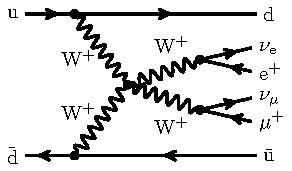
\includegraphics[width=0.30\linewidth]{feynman/LO_EW_5}
          \raisebox{.5ex}{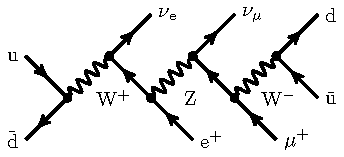
\includegraphics[width=0.35\linewidth]{feynman/LO_EW_2}}
          \raisebox{-1.8ex}{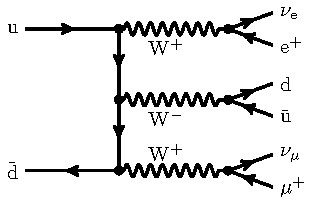
\includegraphics[width=0.32\linewidth]{feynman/LO_EW_3}}
\end{center}
        \caption{Sample tree-level diagrams that contribute to the process $\Pp\Pp\to\mu^+\nu_\mu\Pe^+\nu_{\Pe}\Pj\Pj$ at order $\mathcal{O}{\left(\alpha^{6}\right)}$.
        In addition to typical VBS contributions (left), this order also possesses $s$-channel contributions such as decay chain (middle) and tri-boson contributions (right).}
\label{diag:LO}
\end{figure*}

The scattering of two positively-charged $\PW$ bosons with their subsequent decay into different-flavour leptons 
can proceed at the LHC through the partonic process:
%
\begin{equation}
\Pp\Pp\to\mu^+\nu_\mu{\rm e}^+\nu_{\rm e}\,\Pj\Pj+\mathrm{X}.
\end{equation}

This process possesses three LO contributions of different orders.
At LO, this process can proceed via three different coupling-order combinations:
$\mathcal{O}{\left(\alpha^{6}\right)}$, $\mathcal{O}{\left(\alphas^{2}\alpha^{4}\right)}$, and $\mathcal{O}{\left(\alphas\alpha^{5}\right)}$.
The first, commonly referred to as EW contribution or VBS,\footnote{The name VBS is used even though not all Feynman diagrams involve the scattering
of vector bosons.} receives the contributions from Feynman diagrams such as those in Fig.~\ref{diag:LO}:
in addition to genuine VBS contributions (left diagram), it also features $s$-channel contributions with non-resonant vector bosons 
(center diagram) or from
triple-boson production (right diagram).
Note that $s$-, $t$-, and $u$-channel contributions are defined according to the quark lines.
$s$-channel denotes all Feynman diagrams where the two initial-state partons are connected by a continuous fermion line.
$u$-channel refers to contributions with crossed fermion lines with respect to $t$-channel, which appears for identical quarks or anti-quarks in the final state
The $s$-channel contributions will play a particular role in the study of the various contributions in Sec.~\ref{subsec:contributions}.

When using approximations, care must be taken that only gauge-invariant subsets are considered to obtain physically meaningful results. We will discuss the commonly-used possible choices in detail in the next section.

The second coupling combination corresponds to diagrams with a gluon connecting the two quark lines, and with the $\PW$ bosons 
radiated off the quark lines. Because of the different colour structure, this contribution features a 
different kinematic behaviour than VBS. Nonetheless they share the same final state, and this class of contributions therefore constitutes an irreducible background to the genuine VBS signal.

Finally, the third contribution is the interference of the two types of amplitudes described above.
It is non-zero only for those partonic subprocesses which involve identical quarks or antiquarks.
Such a contribution is typically small but not negligible for realistic experimental set-ups \cite{Biedermann:2017bss}.

In experimental measurements, special cuts, called VBS cuts, are designed to enhance the EW contribution over the QCD one and to suppress the interference.
These cuts are based on the different kinematical behaviour of the contributions.
The EW contribution is characterised by two jets with large rapidities as well as a large invariant mass.
The two $\PW$ bosons are mostly produced centrally.
This is in contrast to the QCD contribution which favours jets in the central region.
Therefore, the event selection usually involves rapidity-difference and invariant-mass cuts for the jets.
Note that, as pointed out in Ref.~\cite{Biedermann:2017bss}, when considering full amplitudes, the separation between EW and QCD production becomes ill
defined.
Hence, combined measurements which are better theoretically defined should be preferably performed by the experimental collaborations at the LHC.




\section{Details of the calculations}
\label{sec:details}

\subsection{Several descriptions for one process}

As mentioned previously, the contribution of main interest in our process is
the scattering of two W gauge bosons, which includes the quartic gauge-boson vertex.
Therefore it is justified to approximate the full EW contributions simply by only these contributions which contain the $2\rightarrow 2$ scattering process as a subpart.
However, this set of contributions is not gauge invariant.
To make it gauge invariant, one should perform an on-shell projection of the incoming W bosons.
Unfortunately, these momenta are space-like and thus a simple on-shell projection is not possible.
Instead, one can keep the W boson legs connected to the external quark line off-shell while the ones connected to the final-state leptons, which are already time-like, are put on-shell.
Then the polarisation of the gauge boson is accommodated following the implementations of Refs.~\cite{Kuss:1995yv,Accomando:2006hq}.
Such an approximation is usually called effective vector-boson approximation (EVBA) \cite{Dawson:1984gx,Duncan:1985vj,Cahn:1983ip}.

A less crude approximation consists in considering all $t$- and $u$- diagrams and squaring them separately, neglecting interference contributions between the two.
These interferences are expected to be small in the VBS fiducial region, as they are both phase-space and colour suppressed.
The $s$-channel squared diagrams and any interferences with $s$-channels are left out as well.
This approximation is often called $t$-/$u$- approximation, VBF, or even VBS approximation.
We will adopt the latter denomination in the following of the article.
Such an approximation is implemented at LO in the computer codes {\sc Bonsay} and {\sc Powheg}.
This approximation is gauge-invariant, which can be seen by considering that the two protons and therefore the two incoming quarks belong to two different, but otherwise identical, copies of the $SU \left(3\right)$ gauge group.

The squared matrix element of the $s$-channel contributions can be added in addition, but all interferences between different kinematic channels are still neglected. This is the level of simulation available in {\sc VBFNLO}.

All other codes ({\sc MG5\_aMC}, {\sc MoCaNLO+Recola}, {\sc PHANTOM}, and {\sc Whizard}) consider all contributions of order $\mathcal{O}{\left(\alpha^{6}\right)}$ as well as all possible interferences.
Note that the final W boson can always be considered either on-shell or off-shell without affecting the previous discussion.
All the codes mentioned here are described in details in the following sub-section.

Moving on to NLO accuracy, one can extend the approximations presented at LO.
The VBS approximation at NLO is straightforward for the virtual contributions, for the real-contributions one must be careful about gluon-initiated processes\footnote{The initial gluon must not couple to the other initial quark, otherwise there are infrared divergences proportional to $s$-channels which do not match with the ones found in the virtual contributions.
The subset of diagrams where all couplings of the initial state gluon to initial state quark are neglected forms a gauge-invariant subset, with the same argument as presented above. This approach is also fully consistent with the picture of two separate SU(3) copies.
}.
This is implemented in {\sc POWHEG}.
This approximation can be used in combination with a double-pole approximation \cite{Dittmaier:2015bfe} for the virtual contribution.
Such an approximation is implemented in {\sc Bonsay}.
In {\sc VBFNLO}, the $s$-channel contributions are available as well and can be
added on top of the VBS approximation. For the real emission diagrams, thereby
as simplification the gluon emission is fully modelled only for initial-state
radiation. The effect of final-state radiation together with the corresponding
virtual contributions is included as a $K$-factor. 

A further refinement is to consider the full real contributions as well as part of the virtual.
In particular one can consider only one-loop amplitudes where there is no gluon exchange between the quarks and assuming a cancellation of the infrared (IR) poles. \MP{True? I cannot remember exactly what is included}.
\MR{What about gauge invariance? A comment about that would be useful as well.}
Such predictions are provided by {\sc MG5\_aMC}.

Finally the full $\mathcal{O}{\left(\alphas \alpha^{6}\right)}$ computation consists also of EW corrections in the virtual as well as real corrections \cite{Biedermann:2017bss}.
Such predictions are provided by the combination {\sc MoCaNLO+Recola} as published in Ref.~\cite{Biedermann:2017bss}.

In Tab.~\ref{tab:wg1_codes} the details of the various codes are reported. In particular, it is specified whether
\begin{itemize}
    \item all $s$- and $t/u$-channel diagrams that lead to the considered final state are included;
    \item interferences between diagrams are included at LO;
    \item diagrams which do not feature two resonant vector bosons are included;
    \item the so-called non-factorisable (NF) QCD corrections, that is the corrections where (real or virtual) gluons are exchanged between different quark lines,
        are included;
    \item EW corrections to the $\mathcal O (\alpha^5\alphas)$ interference are included. These corrections are of the same order as the NLO QCD corrections to
        the  $\mathcal O (\alpha^6$) term.
\end{itemize}

\begin{table*}[ht!]
    \footnotesize
    \begin{tabularx}{\textwidth}{c|c|X|X|X|X|X}
        Code  &  $\mathcal O(\alpha^6)$ $|s|^2/$ $|t|^2/|u|^2$  &  $\mathcal O(\alpha^6)$ interf.  &  Non-res.  & NLO &  NF QCD  &  EW corr. to $\mathcal O(\alphas \alpha^5)$  \\
        \hline
        \hline
        {\sc Bonsay}        &  $t/u$    &  No       &  Yes, virt. No    &  Yes   & No       &  No  \\
        {\sc POWHEG}        &  $t/u$    &  No       &  Yes              &  Yes   & No       &  No  \\
        {\sc MG5\_aMC}      &  Yes      &  Yes      &  Yes              &  Yes   & No virt. &  No \\
        {\sc MoCaNLO+Recola}&  Yes      &  Yes      &  Yes              &  Yes   & Yes      &  Yes  \\
        {\sc PHANTOM}       &  Yes      &  Yes      &  Yes              &  No    & -        & - \\
        {\sc VBFNLO}        &  Yes      &  No       &  Yes              &  Yes   & No       &  No  \\
        {\sc Whizard}       &  Yes      &  Yes      &  Yes              &  No    & -        & - \\
    \end{tabularx}
    \caption{\label{tab:wg1_codes} Summary of the different properties of the codes employed in the comparison.}
\end{table*}


\subsection{Description of the predictions}
\label{subsec:codedescr}

In the following, the codes employed throughout this paper and the approximations implemented in each of them will be discussed:

\begin{itemize}

\item The program {\sc Bonsay} consists of a general-purpose Monte Carlo integrator written by Christopher Schwan and matrix elements taken from different sources:
Born matrix elements are adapted from the program {\sc Lusifer}~\cite{Dittmaier:2002ap}, real matrix elements are written by Marina Billoni, and virtual matrix elements by Stefan Dittmaier.
One loop integrals are evaluated using the {\sc Collier} library~\cite{Denner:2014gla,Denner:2016kdg}.
For the fiducial cross sections it uses the VBS approximation at LO and NLO.
The virtual corrections are additionally approximated using a double-pole approximation.
For more inclusive cross sections at LO the exact matrix elements ($s$-channels, interferences) can also be used.

  \item {\sc MadGraph5\_aMC@NLO}~\cite{Alwall:2014hca} (henceforth {\sc MG5\_aMC}) is an automatic meta-code (a code that generates codes) which makes it possible to simulate any scattering process
      including NLO QCD corrections both at fixed order and including matching to parton showers, using the {\sc MC@NLO}\ method~\cite{Frixione:2002ik}. It makes use of the subtraction method by Frixione, Kunszt and Signer (FKS)~\cite{Frixione:1995ms,
        Frixione:1997np} (automated in the module {\sc MadFKS}~\cite{Frederix:2009yq,
        Frederix:2016rdc}) for regulating IR singularities. The computations of one-loop amplitudes are carried out by switching dynamically between
        two integral-reduction techniques, OPP~\cite{Ossola:2006us} or Laurent-series expansion~\cite{Mastrolia:2012bu},
        and tensor-integral reduction~\cite{Passarino:1978jh,Davydychev:1991va,Denner:2005nn}. These have been automated in the module {\sc MadLoop}~\cite{Hirschi:2011pa}, which
        in turn exploits {\sc CutTools}~\cite{Ossola:2007ax}, {\sc Ninja}~\cite{Peraro:2014cba,
        Hirschi:2016mdz}, {\sc IREGI}~\cite{ShaoIREGI}, or {\sc Collier}~\cite{Denner:2016kdg}, together with an in-house 
        implementation of the {\sc OpenLoops} optimisation~\cite{Cascioli:2011va}. Finally, scale and PDF uncertainties can be obtained in an exact manner via reweighting
        at zero additional CPU cost~\cite{Frederix:2011ss}.\\
        The simulation of VBS at NLO-QCD accuracy can be performed by issuing the following commands in the program interface:
\begin{verbatim}
> set complex_mass_scheme
> import model loop_qcd_qed_sm_Gmu
> generate p p > e+ ve mu+ vm j j QCD=0 [QCD]
> output
\end{verbatim}
  With these commands the complex-mass scheme is turned on, then the NLO-capable model is loaded\footnote{Despite
            the {\tt loop\_qcd\_qed\_sm\_Gmu} model also includes NLO counterterms for computing EW corrections, it is not yet possible to compute such corrections
        with the current public version of the code.}, finally the process code is generated (note the {\tt QCD=0} syntax to select the purely-EW process)
        and written to disk. No approximation is performed for the Born and real-emission matrix elements. 
        For what concerns the virtual matrix element, because of some internal limitations which will be lifted in the future version capable of computing both QCD and EW corrections,
        only loops with QCD-interacting particles are generated. Such an approximation is equivalent to the assumption that the finite part of
        those loops which feature EW bosons is zero. In practice, since a part of the contribution to the single pole is also missing, the internal 
        pole-cancellation check at run time has to be turned off, by setting the value of the {\tt IR\-Pole\-Check\-Threshold} and 
        {\tt Precision\-Virtual\-At\-Run\-Time} parameters in the {\tt Cards\-/FKS\_\-params.dat} file to -1.

\item The program {\sc MoCaNLO+Recola} is made of a flexible Monte Carlo program dubbed {\sc MoCaNLO} and of the matrix element generator {\sc Recola}~\cite{Actis:2012qn,Actis:2016mpe}.
It can compute arbitrary processes for the LHC at both NLO QCD and EW accuracy in the Standard Model.
This is made possible by the fact that {\sc Recola} can compute arbitrary processes at tree and one-loop level in the Standard Model.
To that end, it relies on the {\sc Collier} library \cite{Denner:2014gla,Denner:2016kdg} to numerically evaluate the one-loop scalar and tensor integrals.
In addition, the subtraction of the IR divergences appearing in the real corrections has been automatised thanks to the Catani--Seymour dipole formalism for both QCD and QED \cite{Catani:1996vz,Dittmaier:1999mb}.
The code has demonstrated its ability to compute at NLO high multiplicity processes up to $2 \to 7$ \cite{Denner:2015yca,Denner:2016wet}.
In particular the full NLO corrections to VBS and its irreducible background \cite{Biedermann:2016yds,Biedermann:2017bss} have been obtained thanks to this tool.
One key aspect for these high multiplicity processes is the fast integration which is ensured by using similar phase-space mappings to those of Refs.~\cite{Berends:1994pv,Denner:1999gp,Dittmaier:2002ap}. 
In {\sc MoCaNLO+Recola} no approximation is performed neither at LO nor at NLO.
It implies that, also contributions stemming from EW corrections to the interference are computed.
        
  \item {\sc Phantom}~\cite{Ballestrero:2007xq} is a dedicated tree-level Monte Carlo for six parton final states 
  at $\Pp \Pp,\, \Pp\bar{\Pp}$ and $\Pe^+\Pe^-$ colliders at orders $\mathcal O(\alpha^6)$ and $\mathcal O(\alphas^2\alpha^4)$ including interferences between the two sets of diagrams.
It employs complete tree-level matrix elements in the complex-mass scheme~\cite{Denner:1999gp,Denner:2005fg,Denner:2006ic} computed via the modular helicity formalism~\cite{Ballestrero:1999md,Ballestrero:1994jn}.
The integration uses a multichannel approach~\cite{Berends:1984gf} and an adaptive strategy~\cite{Lepage:1977sw}.
{\sc Phantom} generates unweighted events at parton level for both the SM and a few instances of beyond the Standard Model (BSM) theories.

  \item The {\sc Powheg-Box}~\cite{Nason:2004rx,Frixione:2007vw,Alioli:2010xd} is a framework for matching NLO-QCD calculations with parton showers.
It relies on the user providing the matrix elements and Born phase-space, but will automatically construct FKS \cite{Frixione:1995ms} subtraction terms and the phase space for the real emission.
For the VBS processes all matrix elements are being provided by a previous version of {\sc VBFNLO}~\cite{Arnold:2008rz, Arnold:2011wj, Baglio:2014uba} and hence the approximations used in the {\sc Powheg-Box} are similar to those used in {\sc VBFNLO}.

  \item {\sc VBFNLO}~\cite{Arnold:2008rz, Arnold:2011wj, Baglio:2014uba} is a flexible
    parton-level Monte Carlo for processes with EW bosons. It
    allows the calculation of VBS processes at NLO QCD in the VBS
    approximation, with process IDs between 200 and 290. The corresponding
    $s$-channel contributions are available separately as tri-boson processes with
    semi-leptonic decays, with process IDs in the 400 range\ZM{which range is it?}. These can simply
    be added on top of the VBS contribution. Interferences between the two are therefore neglected.
    The usage of leptonic tensors in the calculation, pioneered in
    Ref.~\cite{Jager:2006zc}, thereby leads to a significant speed improvement over
    automatically generated code.  Besides the SM, also a variety of
    new-physics models including anomalous couplings of the Higgs and gauge
    bosons can be simulated.

  \item {\sc Whizard}~\cite{Moretti:2001zz,Kilian:2007gr} is a multi-purpose
      event generator with the LO matrix element generator {\sc O'Mega}. \ZM{ if NLO results for this processes cannot be provided, we should skip what follows, or at least clarify the limitations}
provides FKS subtraction terms for any NLO process, while virtual matrix
elements are provided externally by {\sc
OpenLoops}~\cite{Cascioli:2011va} (alternatively, {\sc Recola}~\cite{Actis:2012qn,Actis:2016mpe}
(\emph{cf.}\ above) can be used as well). {\sc Whizard} allows to simulate a
huge number of BSM models as well, in particular in
the VBS channel in terms of both higher-dimensional operators as well as explicit
resonances.

\end{itemize}

We conclude this section by summarising the characteristics of the various codes in Tab.~\ref{tab:wg1_codes}.
In particular, it is specified whether
\begin{itemize}
    \item all $s$- and $t/u$-channel diagrams are included;
    \item interferences between different diagrams of diagrams ($s/t/u$-channel) are included at LO;
    \item diagrams which do not feature two resonant vector-bosons are included;
    \item the so-called non-factorisable (NF) QCD corrections, \emph{i.e.}\ the corrections where (real or virtual) gluons are exchanged between different quark lines,
        are included;
    \item EW corrections to the interference of order $\mathcal O (\alpha^5\alphas)$ are included.
    These corrections are of the same order as the NLO QCD corrections to the contribution of order $\mathcal O (\alpha^6$) term.
\end{itemize}

\begin{table*}[ht!]
    \footnotesize
    \begin{tabularx}{\textwidth}{c|c|X|X|X|X|X}
        Code  &  $\mathcal O(\alpha^6)$ $s, t, u$  &  $\mathcal O(\alpha^6)$ interf.  &  Non-res.  & NLO &  NF QCD  &  EW corr. to order $\mathcal O(\alphas \alpha^5)$  \\
        \hline
        \hline
        {\sc Bonsay}        &  $t/u$    &  No       &  Yes, virt. No    &  Yes   & No       &  No  \\
        {\sc Powheg}        &  $t/u$    &  No       &  Yes              &  Yes   & No       &  No  \\
        {\sc MG5\_aMC}      &  Yes      &  Yes      &  Yes              &  Yes   & virt. No &  No \\
        {\sc MoCaNLO+Recola}&  Yes      &  Yes      &  Yes              &  Yes   & Yes      &  Yes  \\
        {\sc PHANTOM}       &  Yes      &  Yes      &  Yes              &  No    & -        & - \\
        {\sc VBFNLO}        &  Yes      &  No       &  Yes              &  Yes   & No       &  No  \\
        {\sc Whizard}       &  Yes      &  Yes      &  Yes              &  No    & -        & - \\
    \end{tabularx}
    \caption{\label{tab:wg1_codes} Summary of the different properties of the computer programs employed in the comparison.}
\end{table*}


\subsection{Input parameters}
\label{subsec:inputpar}

The partonic processes are simulated at the LHC with a center-of-mass energy $\sqrt s = 13 \TeV$.
The NNPDF~3.0 parton density~\cite{Ball:2014uwa} with five flavour scheme, NLO QCD evolution, and a strong coupling constant $\alphas\left( \MZ \right) = 0.118$ is employed.\footnote{The corresponding {\tt lhaid} in LHAPDF6~\cite{Buckley:2014ana} is 260000.}
Since the employed PDF set has no photonic density, photon-induced processes are not considered.
Initial-state collinear singularities are factorised with the ${\overline{\rm MS}}$ scheme, consistently with what is done in NNPDF.

For the mass and width of the massive particles, the following values are used:
%
\begin{alignat}{2}
                  \Mt   &=  173.21\GeV,       & \quad \quad \quad \Gt &= 0 \GeV,  \nonumber \\
                \MZOS &=  91.1876\GeV,      & \quad \quad \quad \GZOS &= 2.4952\GeV,  \nonumber \\
                \MWOS &=  80.385\GeV,       & \GWOS &= 2.085\GeV,  \nonumber \\
                M_{\rm H} &=  125.0\GeV,       &  \GH   &=  4.07 \times 10^{-3}\GeV.
\end{alignat}
%
The measured on-shell (OS) values for the masses and widths of the W and Z bosons are converted into pole values for the gauge bosons ($V=\PW,\PZ$) according to Ref.~\cite{Bardin:1988xt},
%
\begin{equation}
\begin{split}
        M_V &= \MVOS/\sqrt{1+(\GVOS/\MVOS)^2}\,, \\
   \Gamma_V &= \GVOS/\sqrt{1+(\GVOS/\MVOS)^2}.
\end{split}
\end{equation}
%
The EW coupling is renormalised in the $G_\mu$ scheme \cite{Denner:2000bj} where
%
\begin{equation}
    G_{\mu}    = 1.16637\times 10^{-5}\GeV^{-2}.
\end{equation}
%
The numerical value of $\alpha$, corresponding to the choice of input parameters is
%
\begin{equation}
 \alpha = 7.555310522369 \times 10^{-3}.
\end{equation}
The CKM-Matrix is assumed to be diagonal, meaning that the mixing between different quark families is neglected.
The complex-mass scheme~\cite{Denner:1999gp,Denner:2005fg} is used throughout to treat unstable intermediate particles in a gauge-invariant manner.

The renormalisation and factorisation scales are set to the dynamical scale
%
\begin{equation}
\label{eq:defscale}
 \mu_{\rm ren} = \mu_{\rm fac} = \sqrt{p_{\rm T, j_1}\, p_{\rm T, j_2}}.
\end{equation}
%
This choice of scale has been shown to provide stable NLO-QCD predictions \cite{Denner:2012dz}.

Following experimental measurements \cite{Aad:2014zda,Aaboud:2016ffv,Khachatryan:2014sta,CMS:2017adb}, the event selection used in the present study is:

\begin{itemize}
    \item The two same-sign charged leptons are required to have
        \begin{align}
        \label{cut:1}
         \ptsub{\Pl} >  20\GeV,\qquad |y_{\Pl}| < 2.5, \qquad \Delta R_{\Pl\Pl}> 0.3\,.
        \end{align}
    \item The total missing transverse energy, computed from the vectorial sum of the transverse momenta of the two neutrinos, is required to be
        \begin{align}
        \label{cut:2}
          \etsub{\text{miss}}=p_{\rm T, miss} >  40\GeV\,.
        \end{align}
    \item QCD partons (quarks and gluons) are clustered together using the anti-$k_T$ algorithm~\cite{Cacciari:2008gp} with distance parameter $R=0.4$. Jets are required
        to have
        \begin{align}
        \label{cut:3}
         \ptsub{\Pj} >  30\GeV, \qquad |y_\Pj| < 4.5, \qquad \Delta R_{\Pj\Pl} > 0.3 \,.
        \end{align}
        VBS cuts are applied on the two jets with largest transverse-momentum, unless otherwise stated.
        These are an in\-vari\-ant mass cut on the di-jet system as well as rapidity-separation cut between the two jets.
        The nominal values of these cuts if not stated explicitly read:
        \begin{align}
        \label{cut:4}
         m_{\Pj \Pj} >  500\GeV,\qquad |\Delta y_{\Pj \Pj}| > 2.5.
        \end{align}
    \item When EW corrections are computed, real photons and charged fermions are clustered together using the anti-$k_T$ algorithm with
        radius parameter $R=0.1$. In this case, leptons and quarks are understood as {\it dressed fermions}.
\end{itemize}


\section{Leading-order study}
\label{sec:LO}

\subsection{Three contributions}
\label{subsec:contributions}

At tree level, there are three contributions to the $\PW^+\PW^+$ production in association with two jets: the pure EW component $\mathcal{O}(\alpha^6)$, the interference $\mathcal{O}(\alphas\alpha^5)$, and the QCD background $\mathcal{O}(\alphas^2\alpha^4)$.
In the present section, the cross sections and distributions are obtained without applying the VBS cuts on $m_{\Pj\Pj}$ and $|\Delta y_{\Pj\Pj}|$.
In Tab.~\ref{tab:LOscanXsec}, the cross sections of the three contributions are reported.
The EW, QCD, and interference contributions amount to $57\%$, $37\%$, and $6\%$ of the total inclusive cross section, respectively.
The QCD contribution does not posses external gluons due to charge conservation.
Thus the $\mathcal{O}(\alphas^2\alpha^4)$ diagrams only involve gluon exchange in the $t/u$-channel between the quark lines.
This results in a small contribution although the VBS cuts have not been imposed.
The interference between EW and QCD contributions is small, due to color suppression, but not negligible ($t/u$ interference with identical fermions).

\begin{table}[h!]
    \centering
    \begin{tabular}{c|c|c|c}
        Order & $\mathcal{O}(\alpha^6)$ & $\mathcal{O}(\alphas^2\alpha^4)$ & $\mathcal{O}(\alphas\alpha^5)$ \\
        \hline
        \hline
        $\sigma[\rm{fb}]$ & $ 2.292 \pm 0.002 $ & $ 1.477 \pm 0.001 $ & $ 0.223 \pm 0.003 $ \\
%         {\sc Xxx}&  $ \pm $ & $ \pm $ & $ \pm $
    \end{tabular}
    \caption{\label{tab:LOscanXsec} Cross sections at LO accuracy for the three contributions to the process ${\rm p}{\rm p}\to\mu^+\nu_\mu{\rm e}^+\nu_{\rm e}{\rm j}{\rm j}$.
    These results are for the set-up described in Sec.~\ref{subsec:inputpar}, dropping the $m_{\Pj\Pj}$ and $|\Delta y_{\Pj\Pj}|$ cuts.}
\end{table}

In Fig.~\ref{fig:mjjdyjj_1d} these three contributions are shown separately and summed in the differential distribution of the di-jet invariant mass $m_{\Pj\Pj}$ and the rapidity difference $|\Delta y_{\Pj\Pj}|$.
In the distributions in the di-jet invariant mass (left), one can observe that the EW contribution peaks around an invariant mass of about $80\GeV$.
These are due to diagrams where the two jets originate from the decay of a W boson (see middle and right diagrams in Fig.~\ref{diag:LO}).
Note that these contributions are not present in calculations relying on the VBS approximation.
Also, the EW contribution becomes dominant for di-jet invariant mass larger than $500\GeV$.
The same holds true for jet rapidity difference larger than $2.5$ (right).
This clearly explains why these two observables are used to enhanced the EW contribution over the QCD one.
In particular, in order to have a large EW contribution, rather exclusive cuts are required.

\begin{figure*}[hbt]
\centering
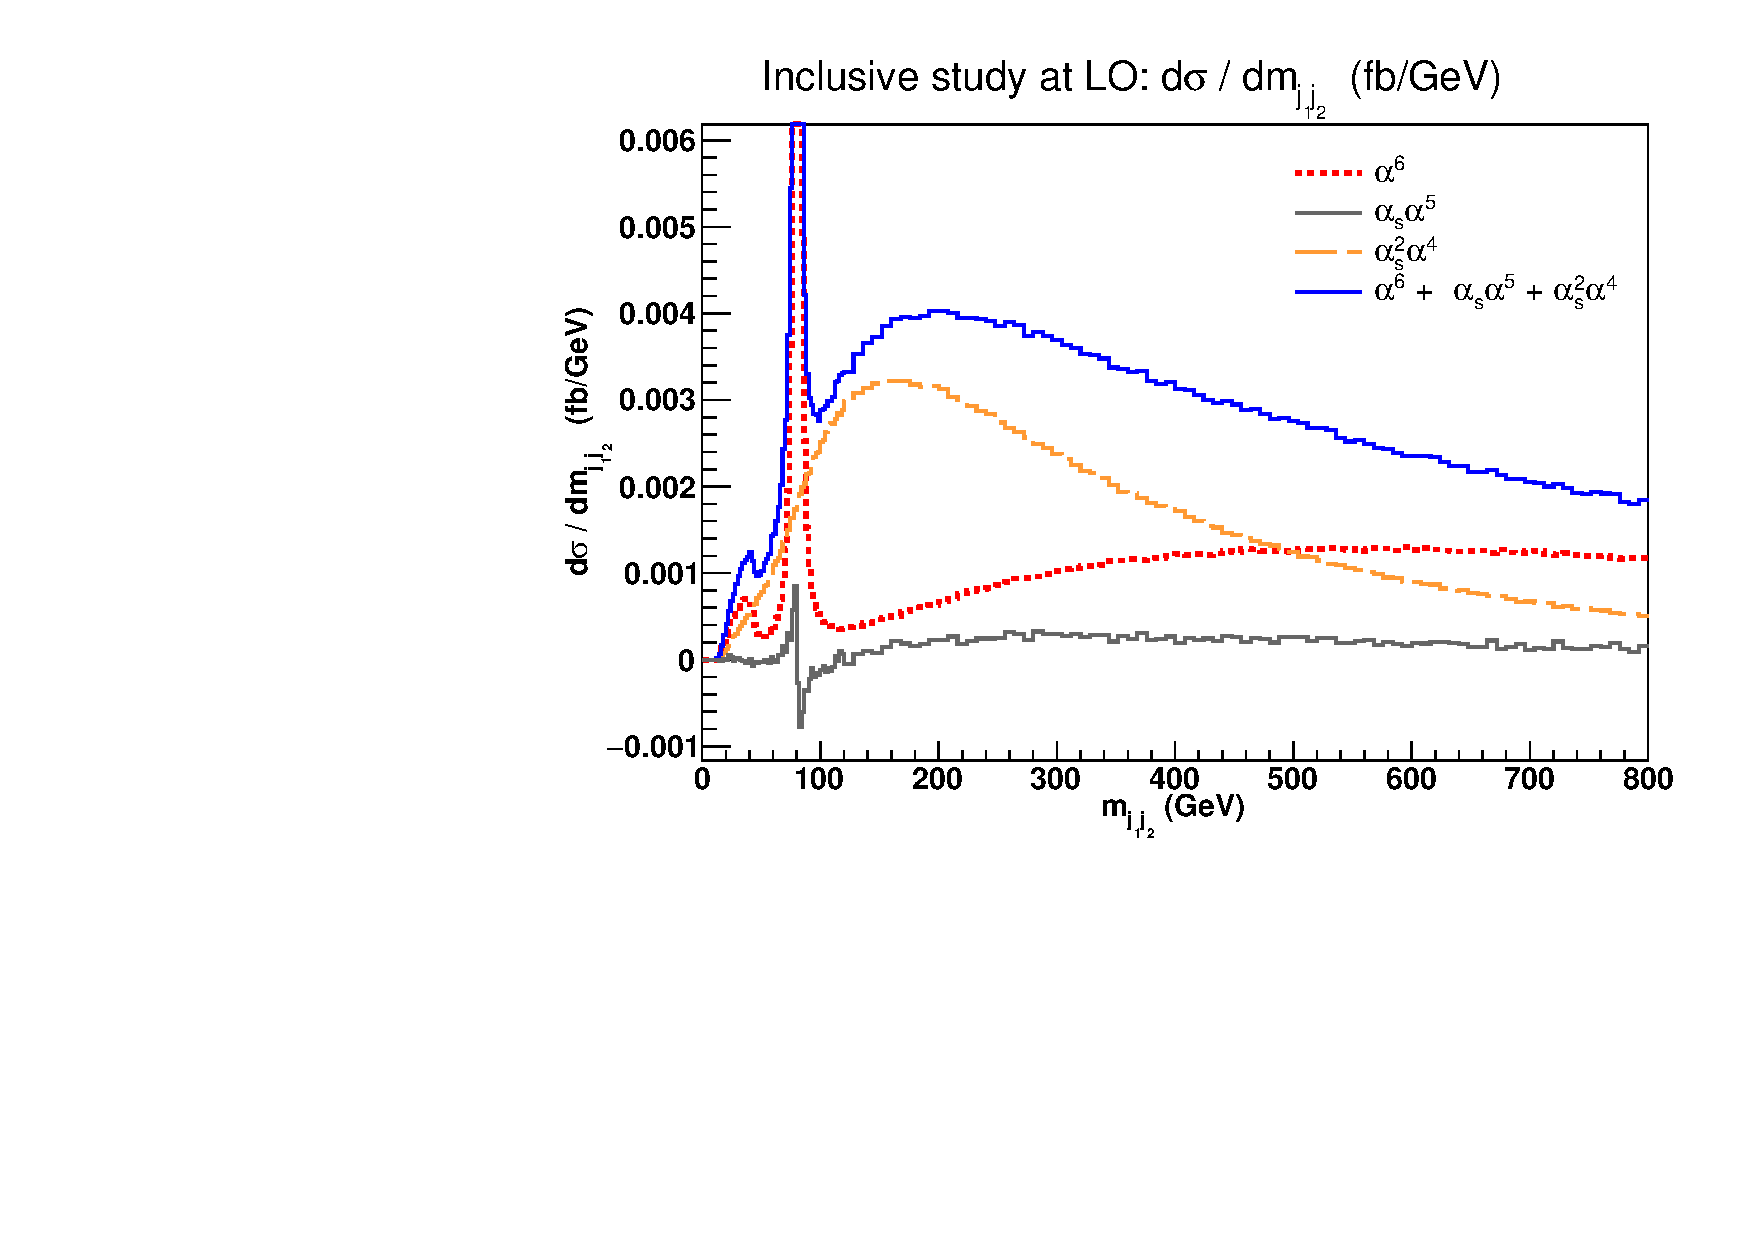
\includegraphics[scale=0.395]{figures/scanfigures/mjj_full.pdf}
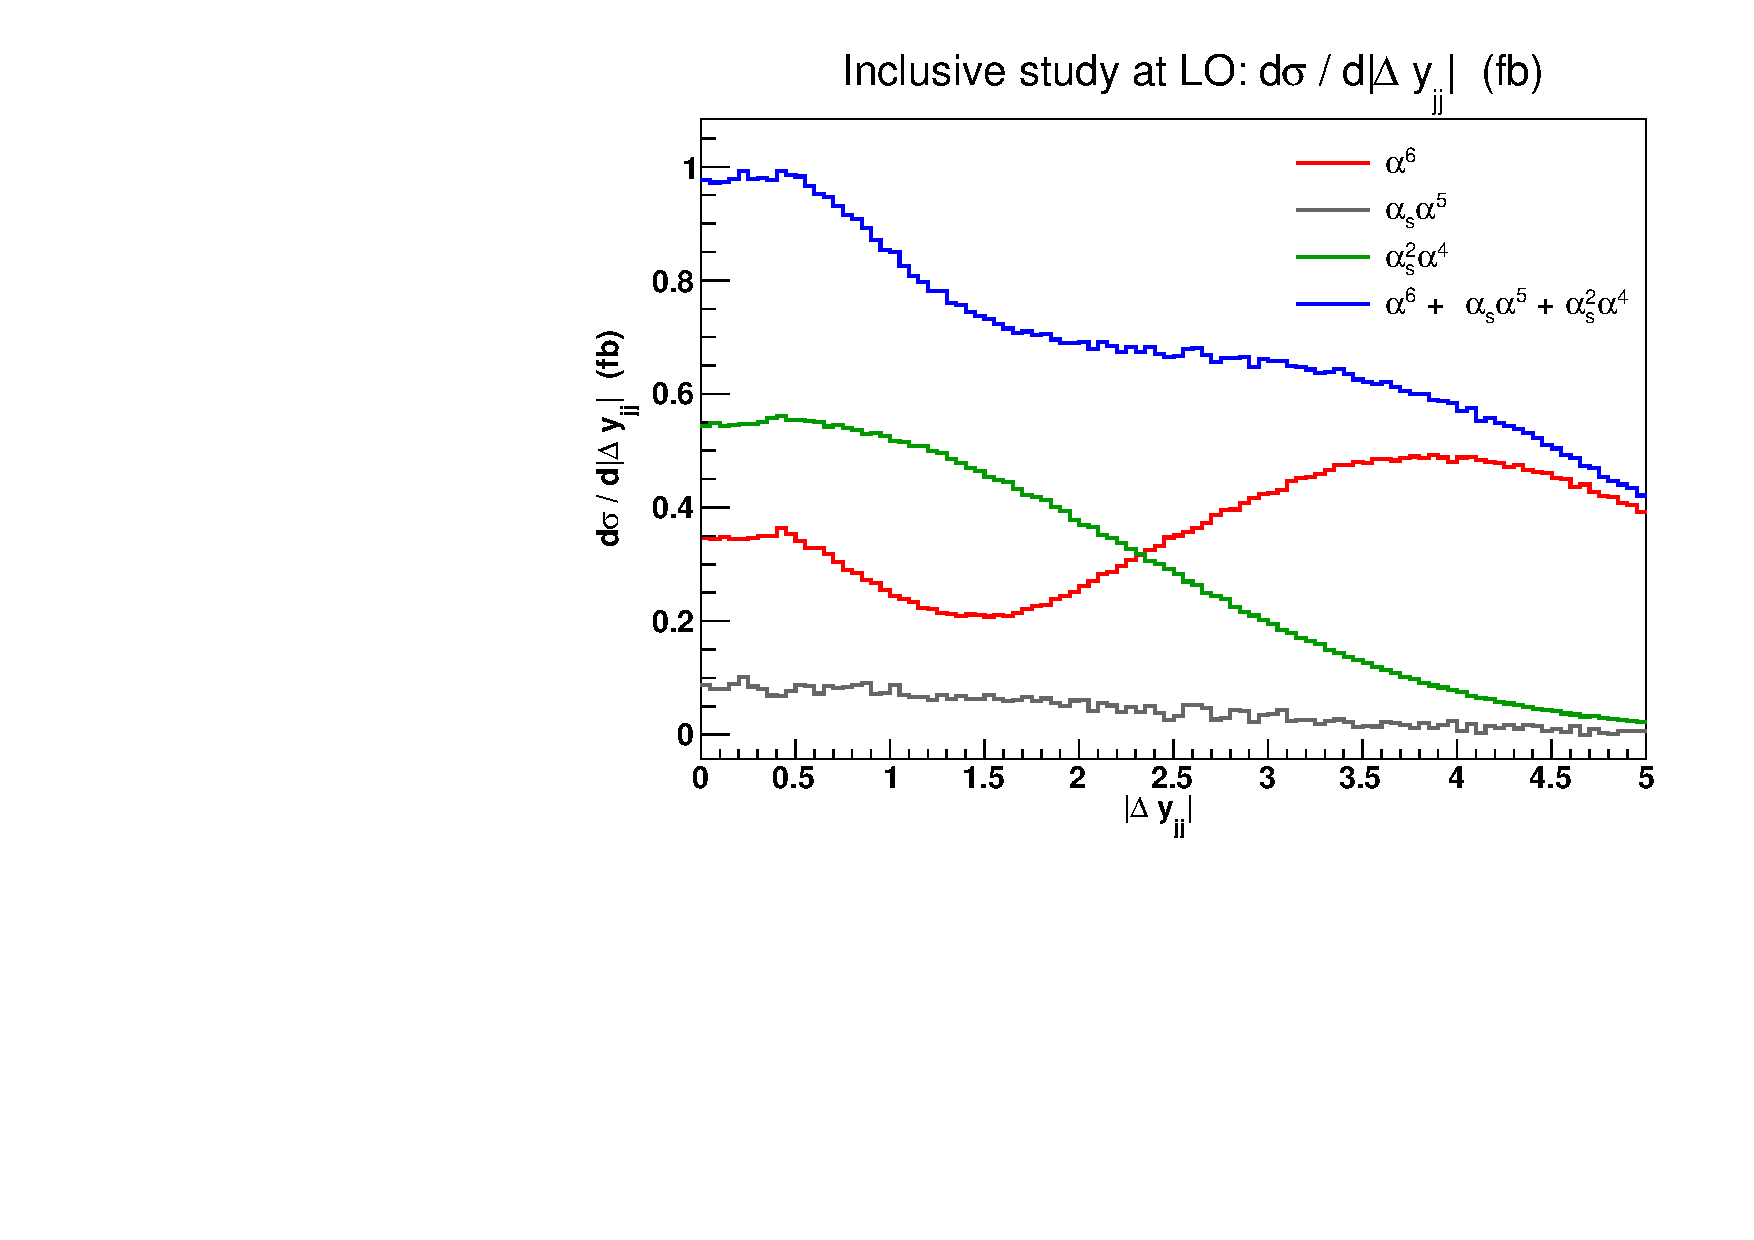
\includegraphics[scale=0.395]{figures/scanfigures/dyjj_full.pdf}
\caption{Differential distribution in the di-jet invariant mass $m_{\Pj\Pj}$ (left) and the difference of the jet rapidities $|\Delta y_{\Pj\Pj}|$ (right) at LO.
The EW contribution is in red, the QCD one in green, and the interference in grey.
The sum of all the contributions is in blue.
No cuts on $m_{\Pj\Pj}$ and $|\Delta y_{\Pj\Pj}|$ are applied.
\MP{On the plots: it should be $\alpha$ and not $\alpha_{em}$ and $m_{\Pj\Pj}$ instead of $M_{jj}$. And we have the convention to put $\alphas$ before $\alpha$.}}
\label{fig:mjjdyjj_1d}
\end{figure*}

This can also be seen in Fig.~\ref{fig:mjjdyjj_2d_LO} where the three contributions are displayed as a function of the di-jet invariant mass and jet rapidity difference.
Again, it is obvious that the region with low di-jet invariant mass and low jet-rapidity difference should be avoided.
This motivates in particular the choice of $m_{\Pj\Pj} > 200\GeV$ and $|\Delta y_{\Pj\Pj}| > 2$ for our inclusive study (see below).
Finally, let us notice that the choice $m_{\Pj\Pj} > 500\GeV$ and $|\Delta y_{\Pj\Pj}| > 2.5$ made by the experimental collaborations is well motivated in order to enhance the EW contribution over its irreducible backgrounds.
These are the cuts used in Sec.~\ref{subsec:LOfiducial}.

\begin{figure}[ht]
\centering
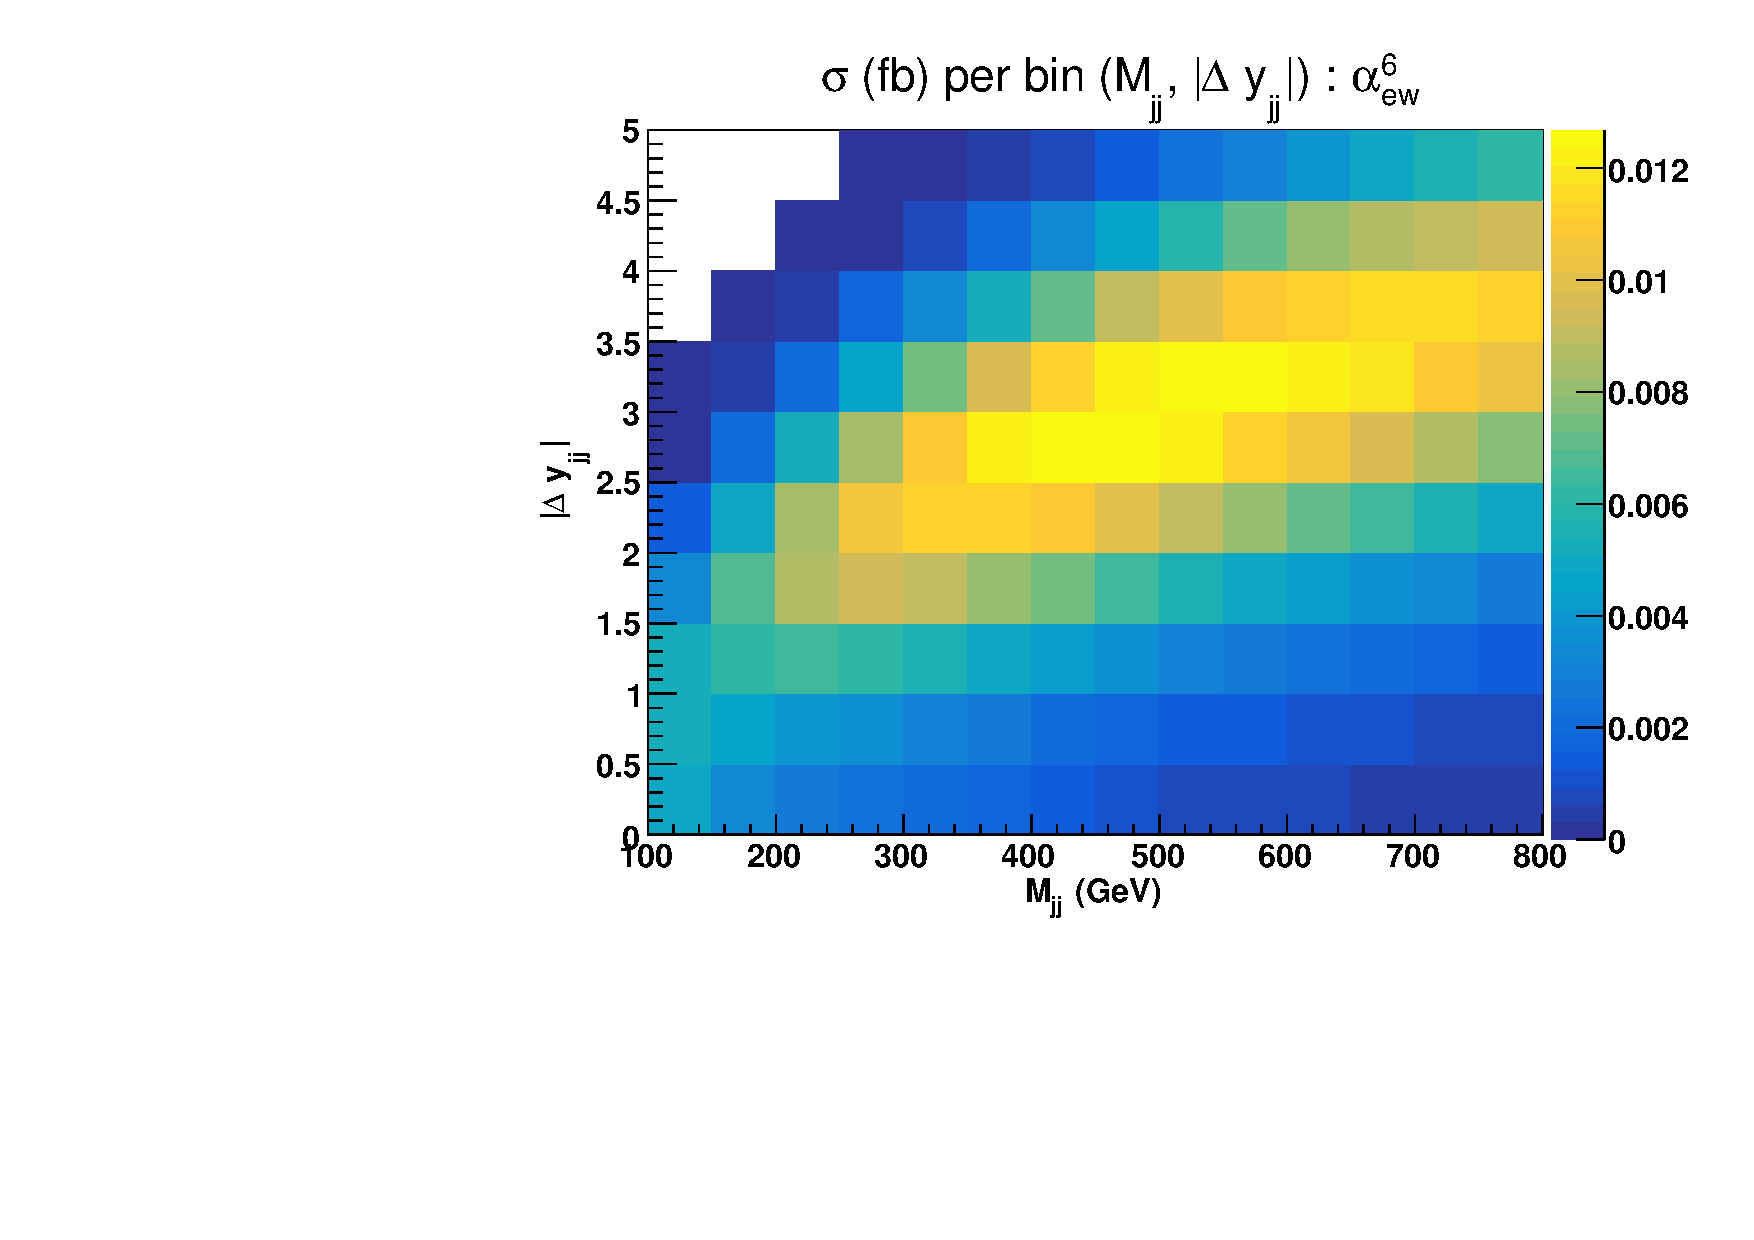
\includegraphics[scale=0.395]{figures/scanfigures/scan_ew6.pdf}
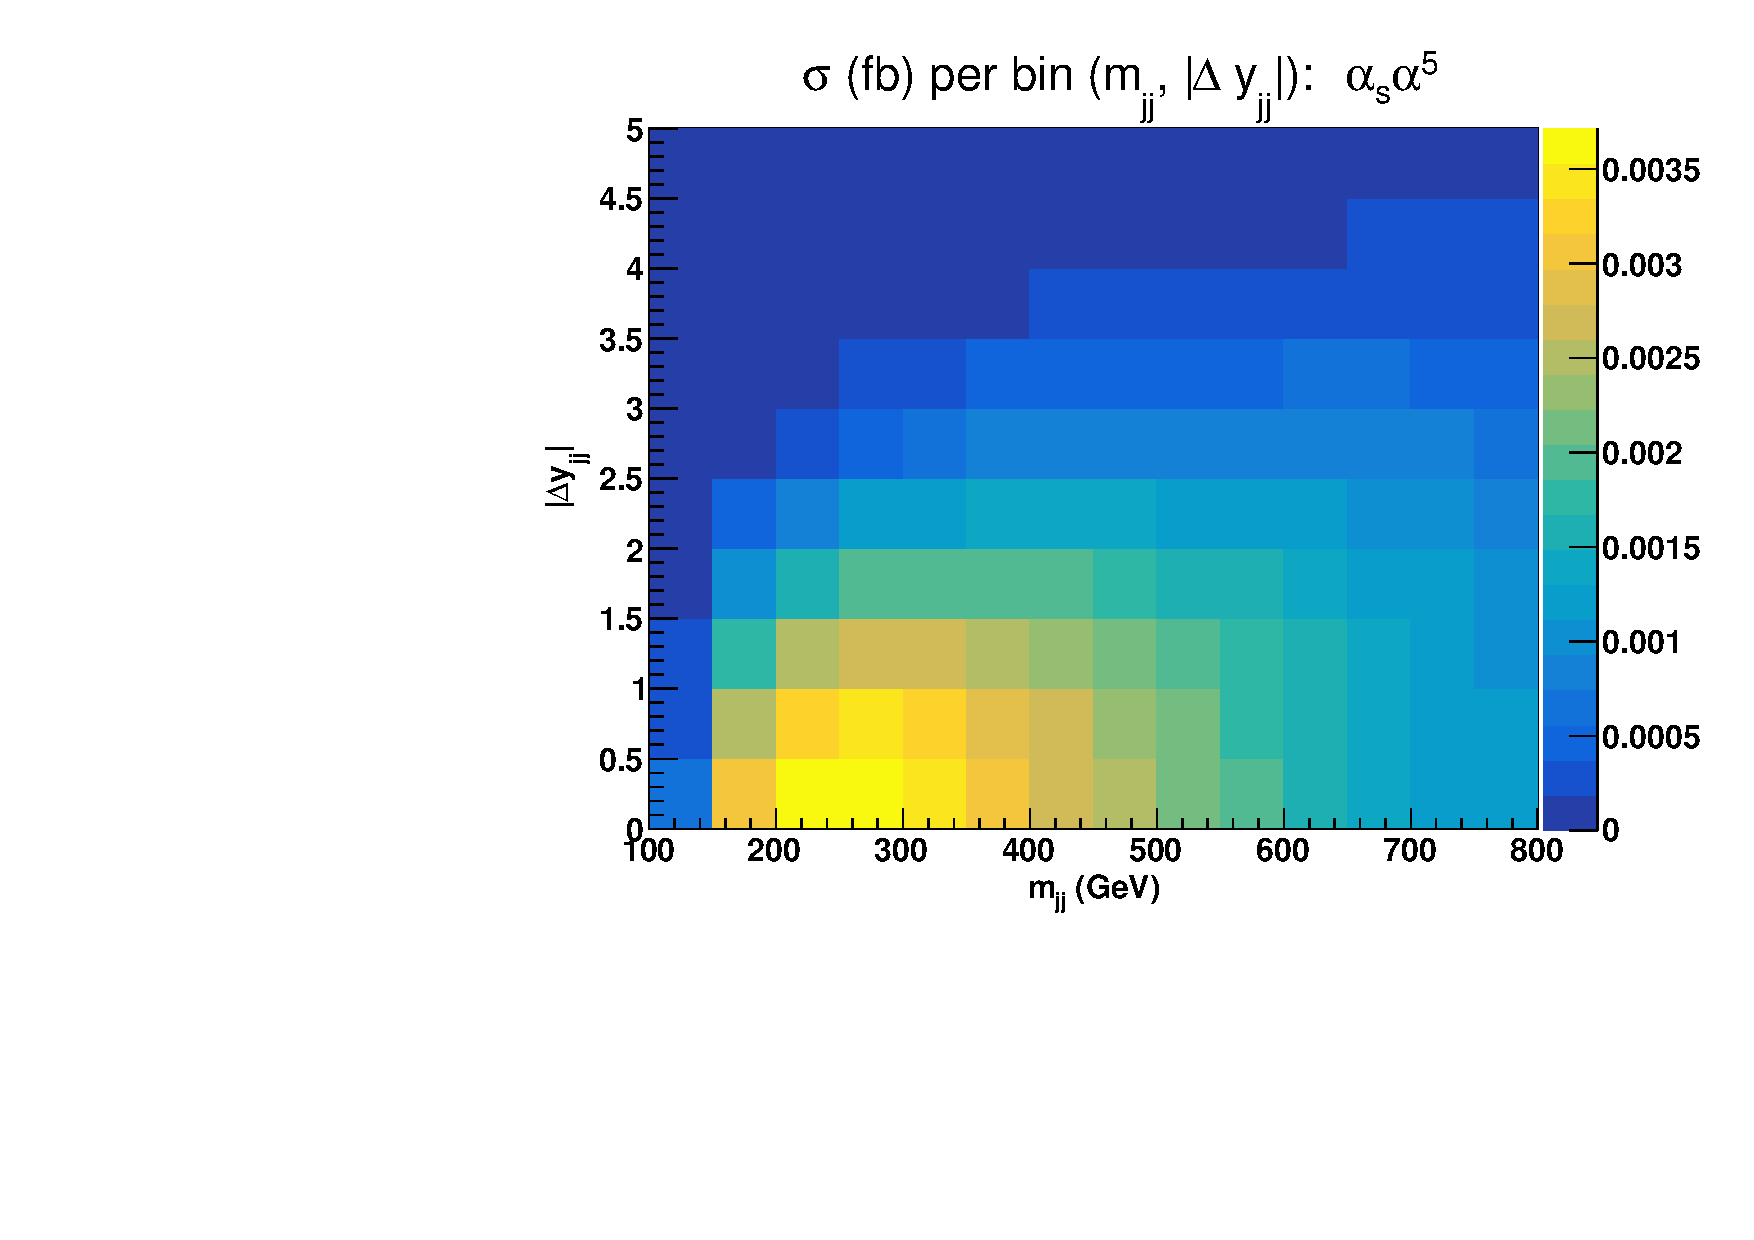
\includegraphics[scale=0.395]{figures/scanfigures/scan_ew5qcd1.pdf}
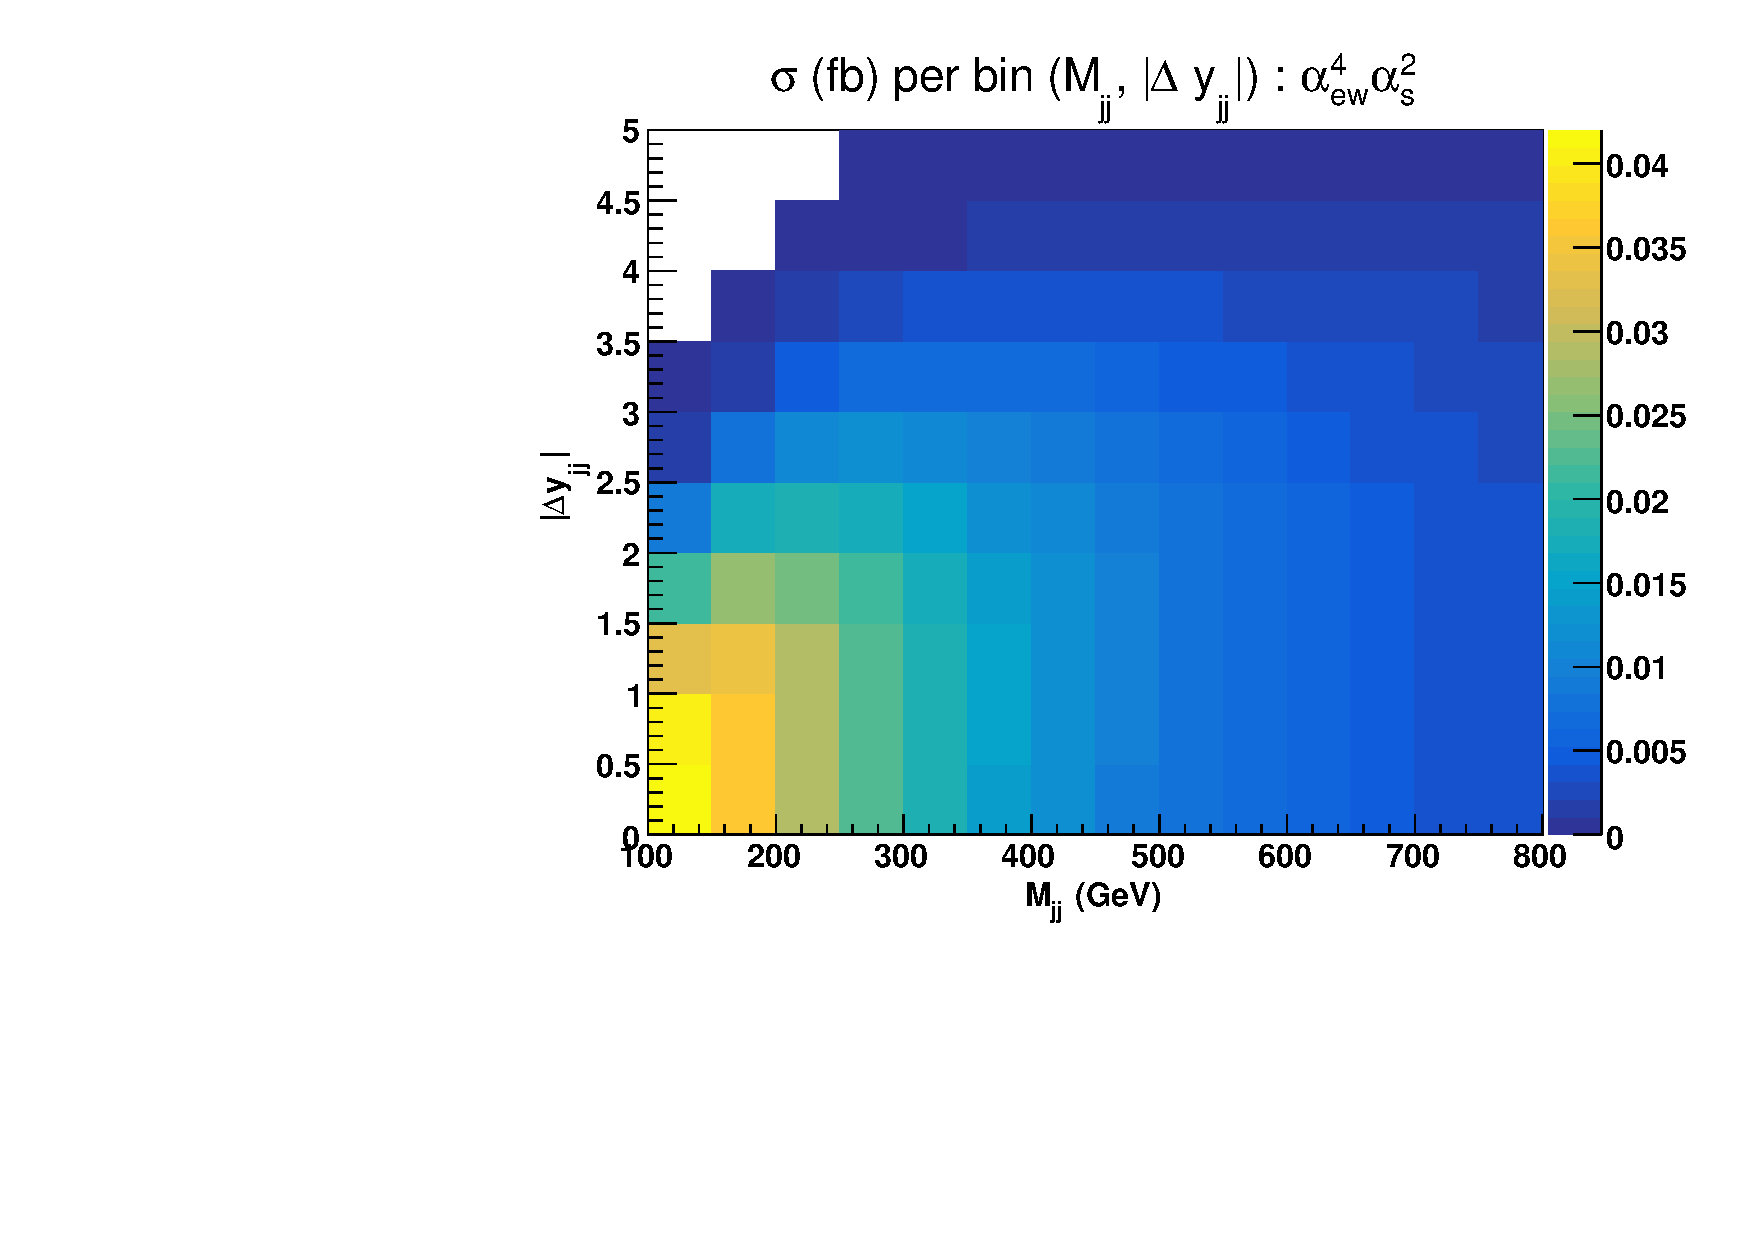
\includegraphics[scale=0.395]{figures/scanfigures/scan_ew4qcd2.pdf}
\caption{Cross sections (fb) per bin in the plan $\left(m_{\Pj\Pj}, \Delta y_{\Pj\Pj}\right)$ for the three LO contributions of orders $\mathcal{O}(\alpha^6)$ (top), $\mathcal{O}(\alphas\alpha^5)$ (middle), and $\mathcal{O}(\alphas^2 \alpha^4)$ (bottom).
\MP{On the plots: it should be $\alpha$ and not $\alpha_{em}$ and $m_{\Pj\Pj}$ instead of $M_{jj}$. And we have the convention to put $\alphas$ before $\alpha$.}}
\label{fig:mjjdyjj_2d_LO}
\end{figure}


\subsection{Inclusive comparison}
\label{subsec:LOinclusive}

As explained previously, the low di-jet invariant mass and low jet rapidity separation is dominated by tri-boson production.
Therefore a comparison of the various approximations in an \emph{inclusive} phase-space volume is performed.
To that end, we have chosen for the inclusive fiducial volume to take the following values for the VBS cuts
\begin{equation}
\label{eq:inclusive}
	m_{jj} > 200\GeV\,,\qquad |\Delta y_{jj}| > 2 .
\end{equation}

The figure showing this is Fig.~\ref{fig:ratio2d_LO}, the ratio of double-differential cross sections in the plan $\left(m_{\Pj\Pj}, \Delta y_{\Pj\Pj}\right)$.
Two plots are displayed: the ratio of the $|t|^2 + |u|^2$ and $|s|^2 + |t|^2 + |u|^2$ approximations over the full calculation, respectively.
In the first case, the approximation is good within $\pm10\%$ over the whole range apart in the low invariant-mass region at both low and large rapidity difference.
The low rapidity difference region possesses remnants of the tri-bosons contributions.
It is therefore expected that the $|t|^2 + |u|^2$ approximation fails in this region.
The second plot, where the $|s|^2 + |t|^2 + |u|^2$ approximation is considered, displays a better behaviour in the previously mentioned region.
The full calculation is approximated at the level of $\pm10\%$ everywhere apart in the upper left corner where the inclusion of $s$-channel contributions did not improve the approximation.
This is due to ...

\begin{figure}[hbt]
\centering
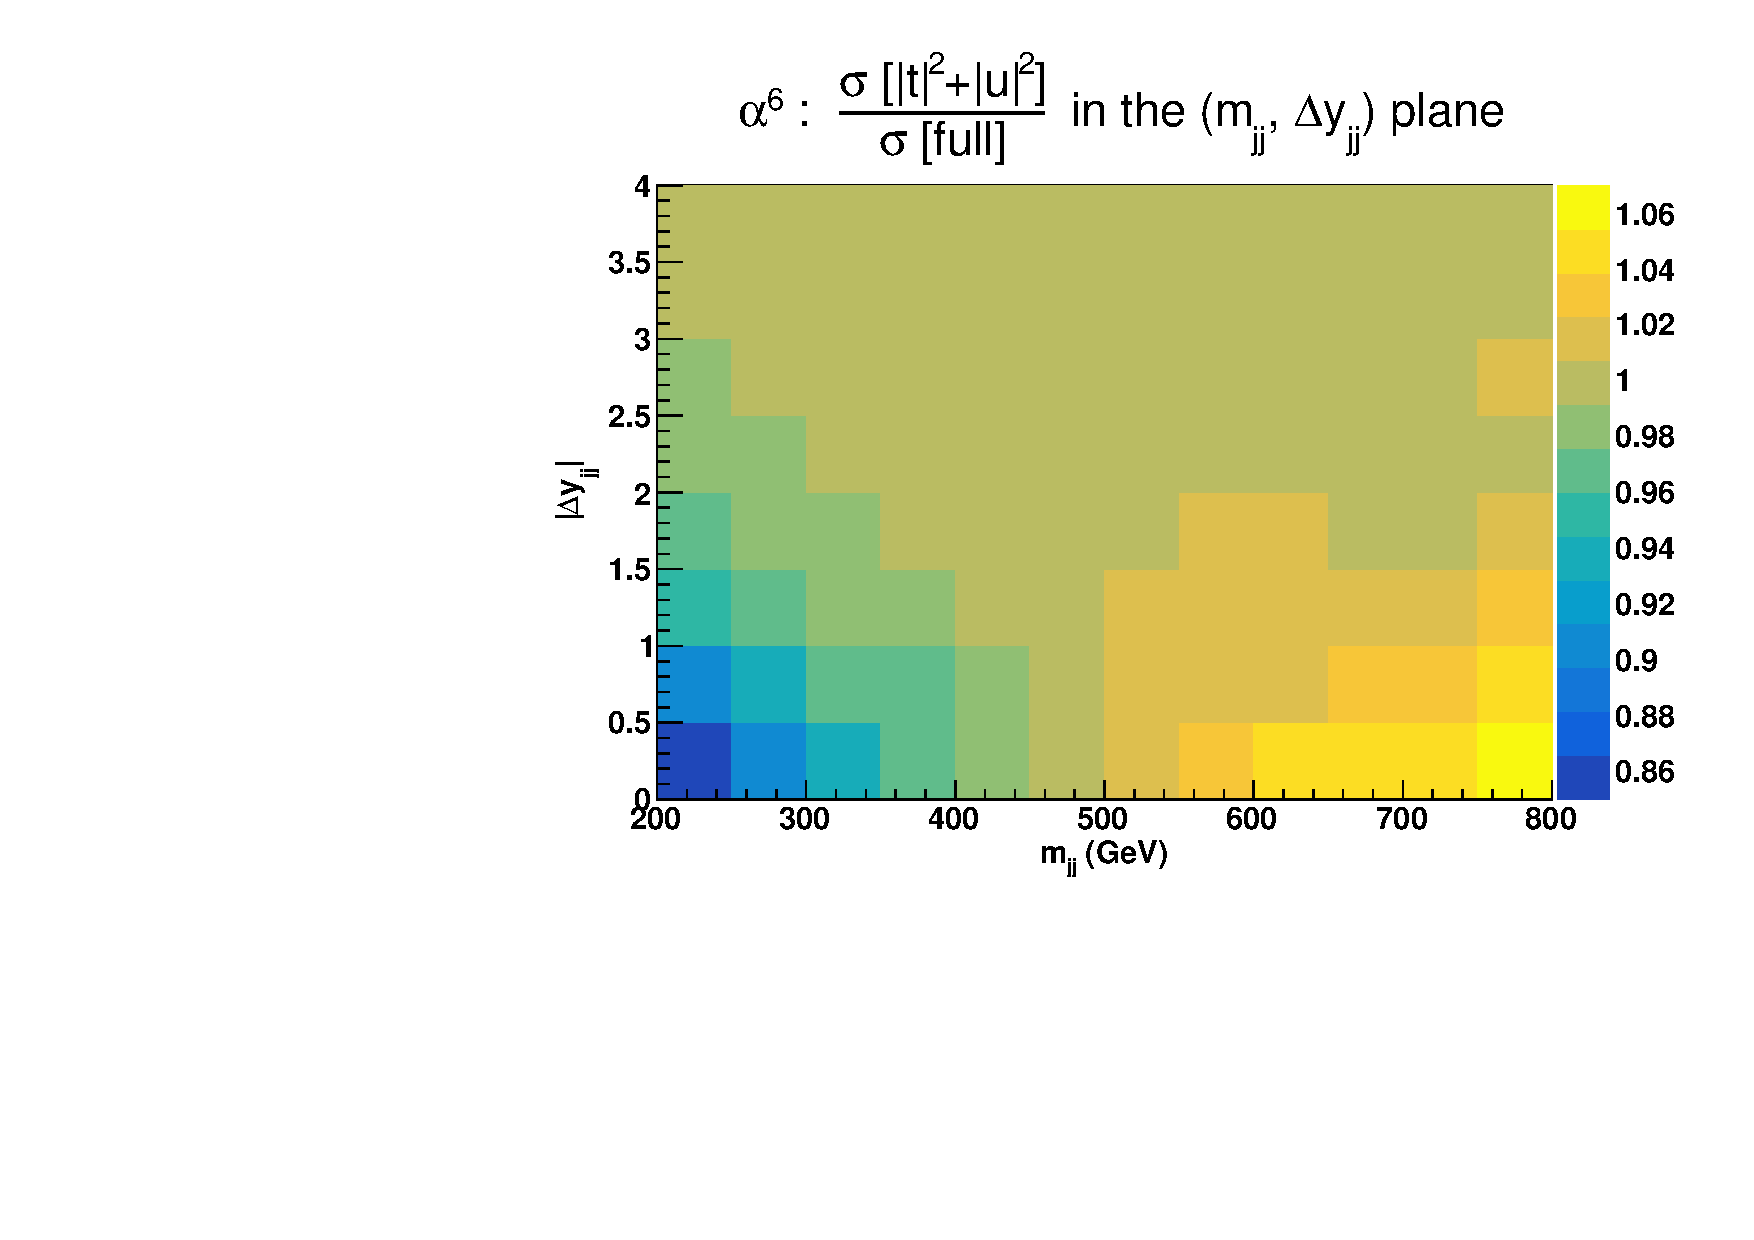
\includegraphics[scale=0.395]{figures/scanfigures/ratio_tu.pdf}
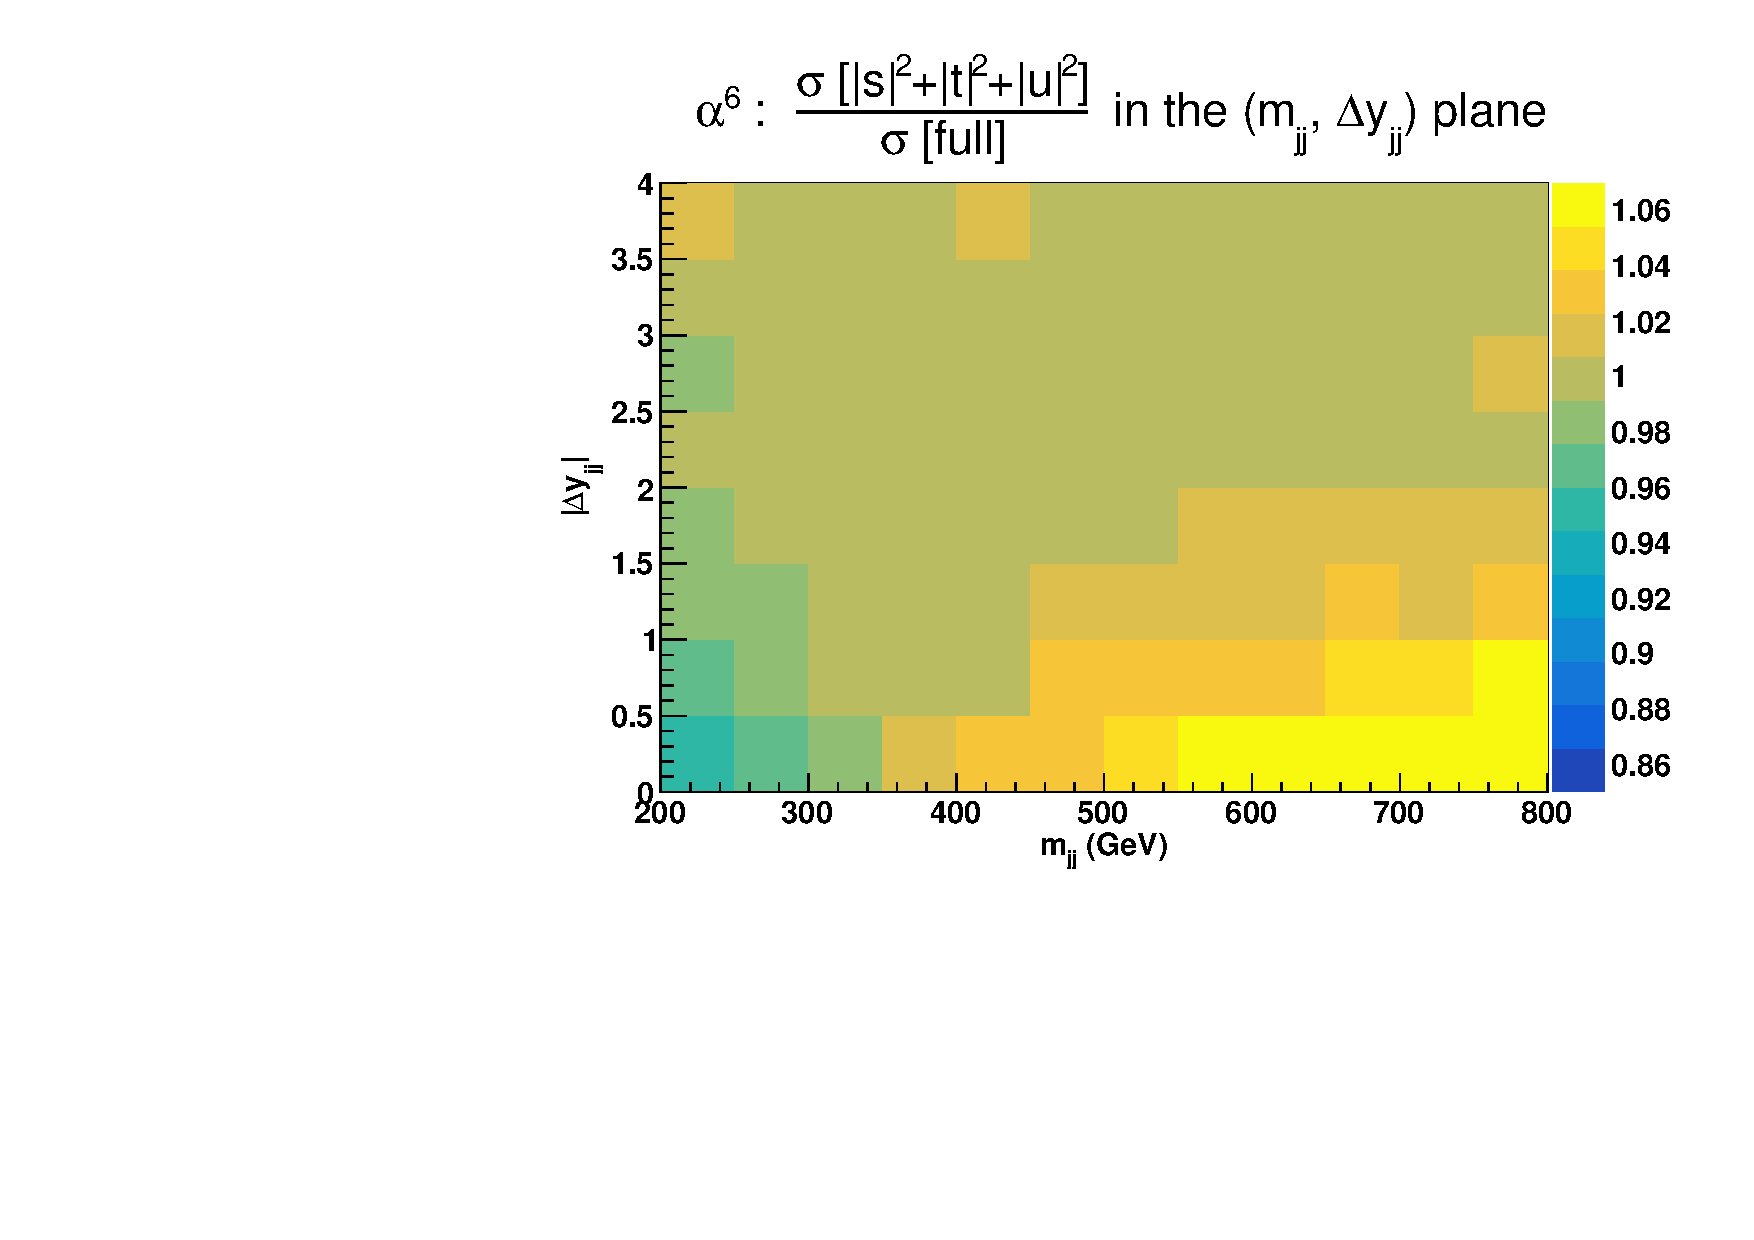
\includegraphics[scale=0.395]{figures/scanfigures/ratio_stu.pdf}
\caption{Cross sections (fb) per bin in the plan $\left(m_{\Pj\Pj}, \Delta y_{\Pj\Pj}\right)$ at order $\mathcal{O}(\alpha^6)$.
Ratio of approximated squared amplitudes over the full matrix element. The approximated squared amplitudes are computed as $|\mathcal{A}|^2 \sim |t|^2 + |u|^2$ (top) and $|\mathcal{A}|^2 \sim |s|^2 + |t|^2 + |u|^2$ (bottom).}
\label{fig:ratio2d_LO}
\end{figure}


\subsection{Comparison in the fiducial region}
\label{subsec:LOfiducial}

In Tab.~\ref{tab:wg1_LOrates}, we report the total rates at LO accuracy obtained with the set-up described in Eqs.~(\ref{cut:1}-\ref{cut:3}) with the VBS cuts $m_{\Pj\Pj} > 500 \GeV$ and $|\Delta y_{\Pj\Pj}| > 2.5$ (see Eq.~(\ref{cut:4})).
The order considered here is the order $\mathcal{O}(\alpha^6)$.
We note that several full predictions are not in statistical agreement. These are possibly due to Monte-Carlo 
integrators performing too aggressive estimations of statistical uncertainties. Nonetheless, all these predictions agree within less than $0.5\%$.
At the level of the cross section, it seems difficult to infer the quality of the the various approximations.
This simply means that the details of the various VBS approximations have an impact not larger than $0.5\%$ at 
the level of the fiducial cross section at LO for a typical phase-space volume used by experimental collaborations. This is in agreement with the findings of Ref.~\cite{Oleari:2003tc}.

\begin{table}[h!]
    \centering
    \begin{tabular}{c|r@{ $\pm$ }l}
      Code  &  \multicolumn{2}{c}{$\sigma[\rm{fb}]$}  \\
        \hline
        \hline
        {\sc Bonsay}  &  $1.43636 \pm 0.00002$ \\
        {\sc MG5\_aMC}&  $1.435$ & $0.004$ TO BE UPDATED  \\
        {\sc MoCaNLO+Recola}  &  $1.4347\phantom{0}$ & $0.0001$ \\
        {\sc PHANTOM} &  $1.4374\phantom{0}$ & $0.0006 $  \\
        {\sc Powheg-Box}  &  $1.44092$ & $0.00009$ \\
        {\sc VBFNLO}  &  $1.43796$ & $0.00005$ \\
        {\sc Whizard} &  $1.4381\phantom{0}$ & $0.0002 $
    \end{tabular}
    \caption{\label{tab:wg1_LOrates} Cross sections for the LHC process ${\rm p}{\rm p}\to\mu^+\nu_\mu{\rm e}^+\nu_{\rm e}{\rm j}{\rm j}$ at LO accuracy and order $\mathcal{O}(\alpha^6)$.
    The uncertainties shown refers to the estimated statistical error of the Monte Carlo programs.
    The predictions are obtained in the fiducial region described in Sec.~\ref{subsec:inputpar}.
    \MP{Please add or check your respective numbers}}
\end{table}


In Fig.~\ref{fig:wg1_mjj-llLO}, we show the distributions in the invariant mass (top) and the rapidity difference of the two tagging jets (bottom) which are key observables for VBS measurements.
In both cases we show the absolute distributions in the upper plot, while the lower plot displays the ratio over {\sc VBFNLO} \MP{To be changed to Recola}.
For both observables we find a relatively good agreement among the various tools, which confirms the fact that contributions from $s$-channel diagrams as well as from non-resonant configurations are suppressed in the fiducial region.
In general, the agreement is at the level of $1\%$ or below for each bin.
We have checked that the same level of agreement holds for other standard differential distributions such as rapidity, invariant mass, or transverse momentum.
This means that at LO, in the fiducial volume and for energies relevant to the LHC, the VBS approximation is good to a per cent.
\MP{Add some comment with respect to the 2D scan.}

 \begin{figure*}[htb!]
   \centering
   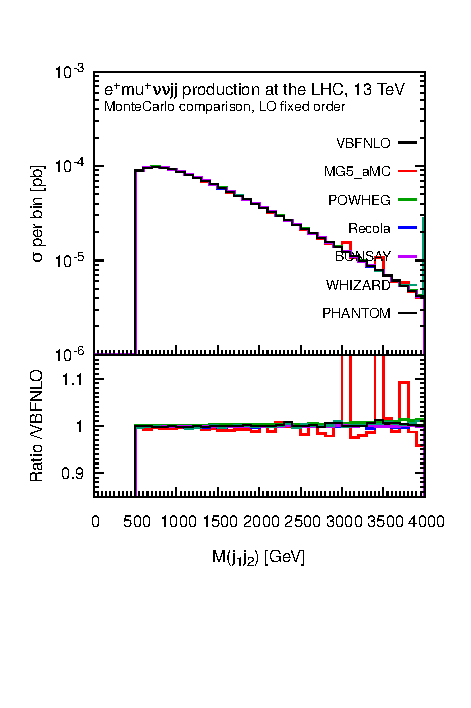
\includegraphics[width=0.4\textwidth,angle=0,clip=true,trim={0.4cm 2cm 0.cm 1.cm}]{figures/LO/mjj_LO.pdf}
   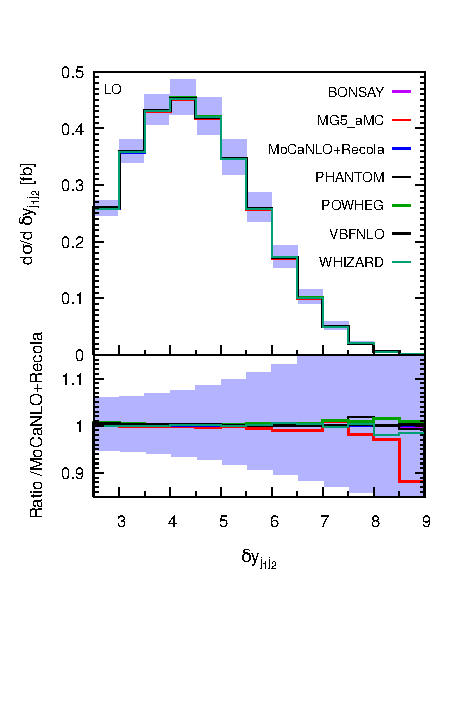
\includegraphics[width=0.4\textwidth,angle=0,clip=true,trim={0.4cm 2cm 0.cm 1.cm}]{figures/LO/dyj1j2_LO.pdf}
\caption{\label{fig:wg1_mjj-llLO} Differential distributions in the invariant mass (top) and rapidity difference of the two tagging jets (bottom).
The LHC process considered is ${\rm p}{\rm p}\to\mu^+\nu_\mu{\rm e}^+\nu_{\rm e}{\rm j}{\rm j}$ at LO accuracy and order $\mathcal{O}(\alpha^6)$.
The description of the different programs used can be found in Sec.~\ref{subsec:codedescr}.
The upper plots provides the absolute value for each prediction while the lower plots presents all predictions normalised to {\sc MoCaNLO}+{\sc Recola} which is one of the full predictions.
The predictions are obtained in the fiducial region described in Sec.~\ref{subsec:inputpar}.
\MP{MG statistics should be improved and the baseline changed to Recola.}
}
\end{figure*}


\section{Next-to-leading order QCD}
\label{sec:NLO}

\subsection{Inclusive comparision}
\label{subsec:NLOinclusive}

According to the results shown in Sec.~\ref{subsec:LOinclusive}, the VBS approximation at LO fails drastically in the region $m_{\Pj\Pj} < 200$ GeV, $|\Delta y_{\Pj\Pj}| < 2$.
Therefore, we present an inclusive study at NLO QCD for the EW component, namely the order $\mathcal{O}(\alphas\alpha^6)$ for the set-up described in Sec.~\ref{subsec:inputpar} but imposing $m_{\Pj\Pj}>200 \GeV$ and $|\Delta y_{\Pj\Pj}|>2$.


% For the inclusive region (see Eq.~\eqref{eq:inclusive}), this approximation is good up to $\pm10\%$ apart for large di-jet differences and low di-jet invariant mass.
% It is therefore interesting to check how good this approximation performs at NLO.
% Thus, we impose the same kinematic cuts shown in Sec.~\ref{subsec:inputpar} and apply the VBS cuts of Eq.~\eqref{eq:inclusive}.

We compare three different predictions at NLO QCD: 
the VBS approximation (dubbed $|t|^2+|u|^2$) implemented in {\sc Bonsay}, the VBS approximation with the $s$-channel contributions from {\sc VBFNLO} (dubbed $|s|^2+|t|^2+|u|^2$), and the full computation.
The full computation employs full matrix elements meaning that $t/u/s$ interferences, factorisable, and non-factorisable QCD corrections as well as EW corrections to the order $\mathcal{O}(\alphas \alpha^5)$ are included.
% This means that in order to cancel all IR singularities, also EW correction to the $\mathcal{O}(\alphas\alpha^5)$ interference have to be included \cite{Biedermann:2016yds}.

The total cross sections within the above mentioned kinematic cuts are shown in Tab.~\ref{tab:crosssecINCLUSIVE}.
The $|t|^2+|u|^2$ approximation for NLO QCD predictions is lower by about $6\%$ with respect to the full calculation.
The inclusion of $s$-channel diagrams improves the approximate prediction, leading to a slight excess at the $2\%$-level.

\begin{table}[h!]
\centering
\begin{tabular}{c|c|c}
Prediction & $\sigma_{\textrm{tot}}\,[\textrm{fb}]$ & $\delta [\%]$ \\
\hline
\hline
full &  $1.733\phantom{0} \pm 0.002\phantom{0}$ & - \\
\hline
$|t|^2 + |u|^2$ & $1.6292 \pm 0.0001$  &  $-6$ \\
\hline
$|s|^2 + |t|^2 + |u|^2$ & $1.7780 \pm 0.0001$  & $+2$
\end{tabular}
\caption{Cross sections at NLO QCD \emph{i.e.}\ at order $\mathcal{O}(\alphas\alpha^6)$ for the full computation and two approximations.
In addition to the cuts of Sec.~\ref{subsec:inputpar}, the VBS cuts take the values $m_{\Pj\Pj}>200 \GeV$ and $|\Delta y_{\Pj\Pj}|>2$.
The uncertainties shown refer to the estimated statistical error of the Monte Carlo programs.}
\label{tab:crosssecINCLUSIVE}
\end{table}

These differences are much more evident in differential distributions.
In Fig.~\ref{fig:mjjdyjj_1d_1}, we show the distributions in the di-jet invariant mass $m_{\Pj\Pj}$ and rapidity separation $|\Delta y_{\Pj\Pj}|$.
For large $m_{\Pj\Pj}$ and large $|\Delta y_{\Pj\Pj}|$, as expected, the VBS approximation is performing well and its $s$-channel extension agrees with the full calculation within $10\%$ per cent.
% On the other hand, for low invariant and low rapidity separation the the VBS approximation is failing at a level of at least $30\%$.
% In this very same region, the VBS approximation with $s$-channel is good within $10\%$.
This is in contrast with the region  $200 \GeV < m_{\Pj\Pj} < 500 \GeV$ and $2<|\Delta y_{\Pj\Pj}|<2.5$, where
the difference between the $|t|^2+|u|^2$ approximation and the full computation can reach $30\%$.
The inclusion of $s$-channels cures partly this behaviour in this region.
Still, for the very low $m_{\Pj\Pj}$ a difference of more than $10\%$ remains.
This tends to indicate that interference contributions and/or non-factorisable QCD corrections play a non-negligible role in this phase-space region.

In order to investigate further the jet-pair kinematics, we look at the double-differential distribution in the variables $m_{\Pj\Pj}$ and $|\Delta y_{\Pj\Pj}|$.
In particular, we compute in each bin the ratio of the approximated cross sections over the full one.
In Fig.~\ref{fig:ratio2d_NLO} we show the ratio $\sigma(|t|^2+|u|^2)/\sigma(\textrm{full})$ and $\sigma(|s|^2+|t|^2+|u|^2)/\sigma(\textrm{full})$.


\begin{figure*}[hbt]
\centering
{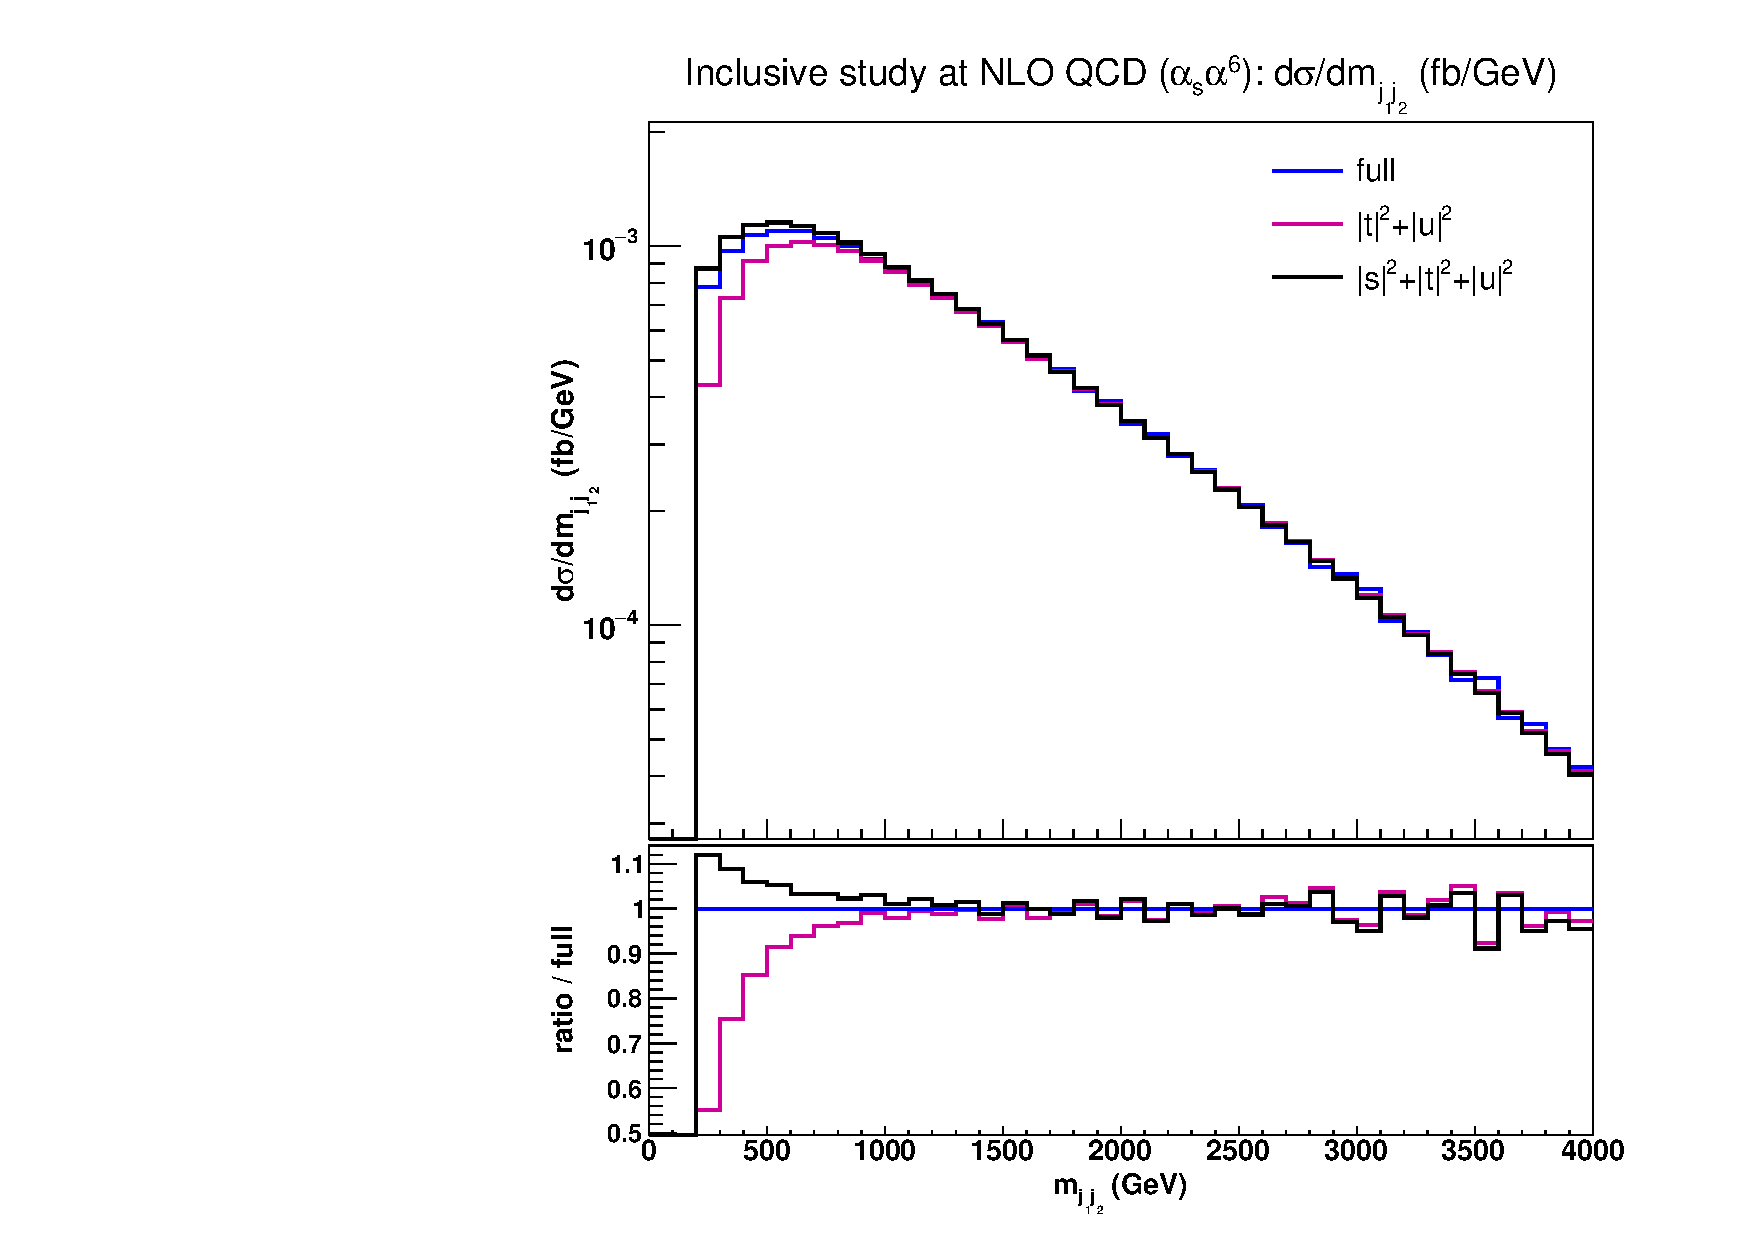
\includegraphics[scale=0.35]{figures/scanfigures/mjj_nlo.pdf}}
{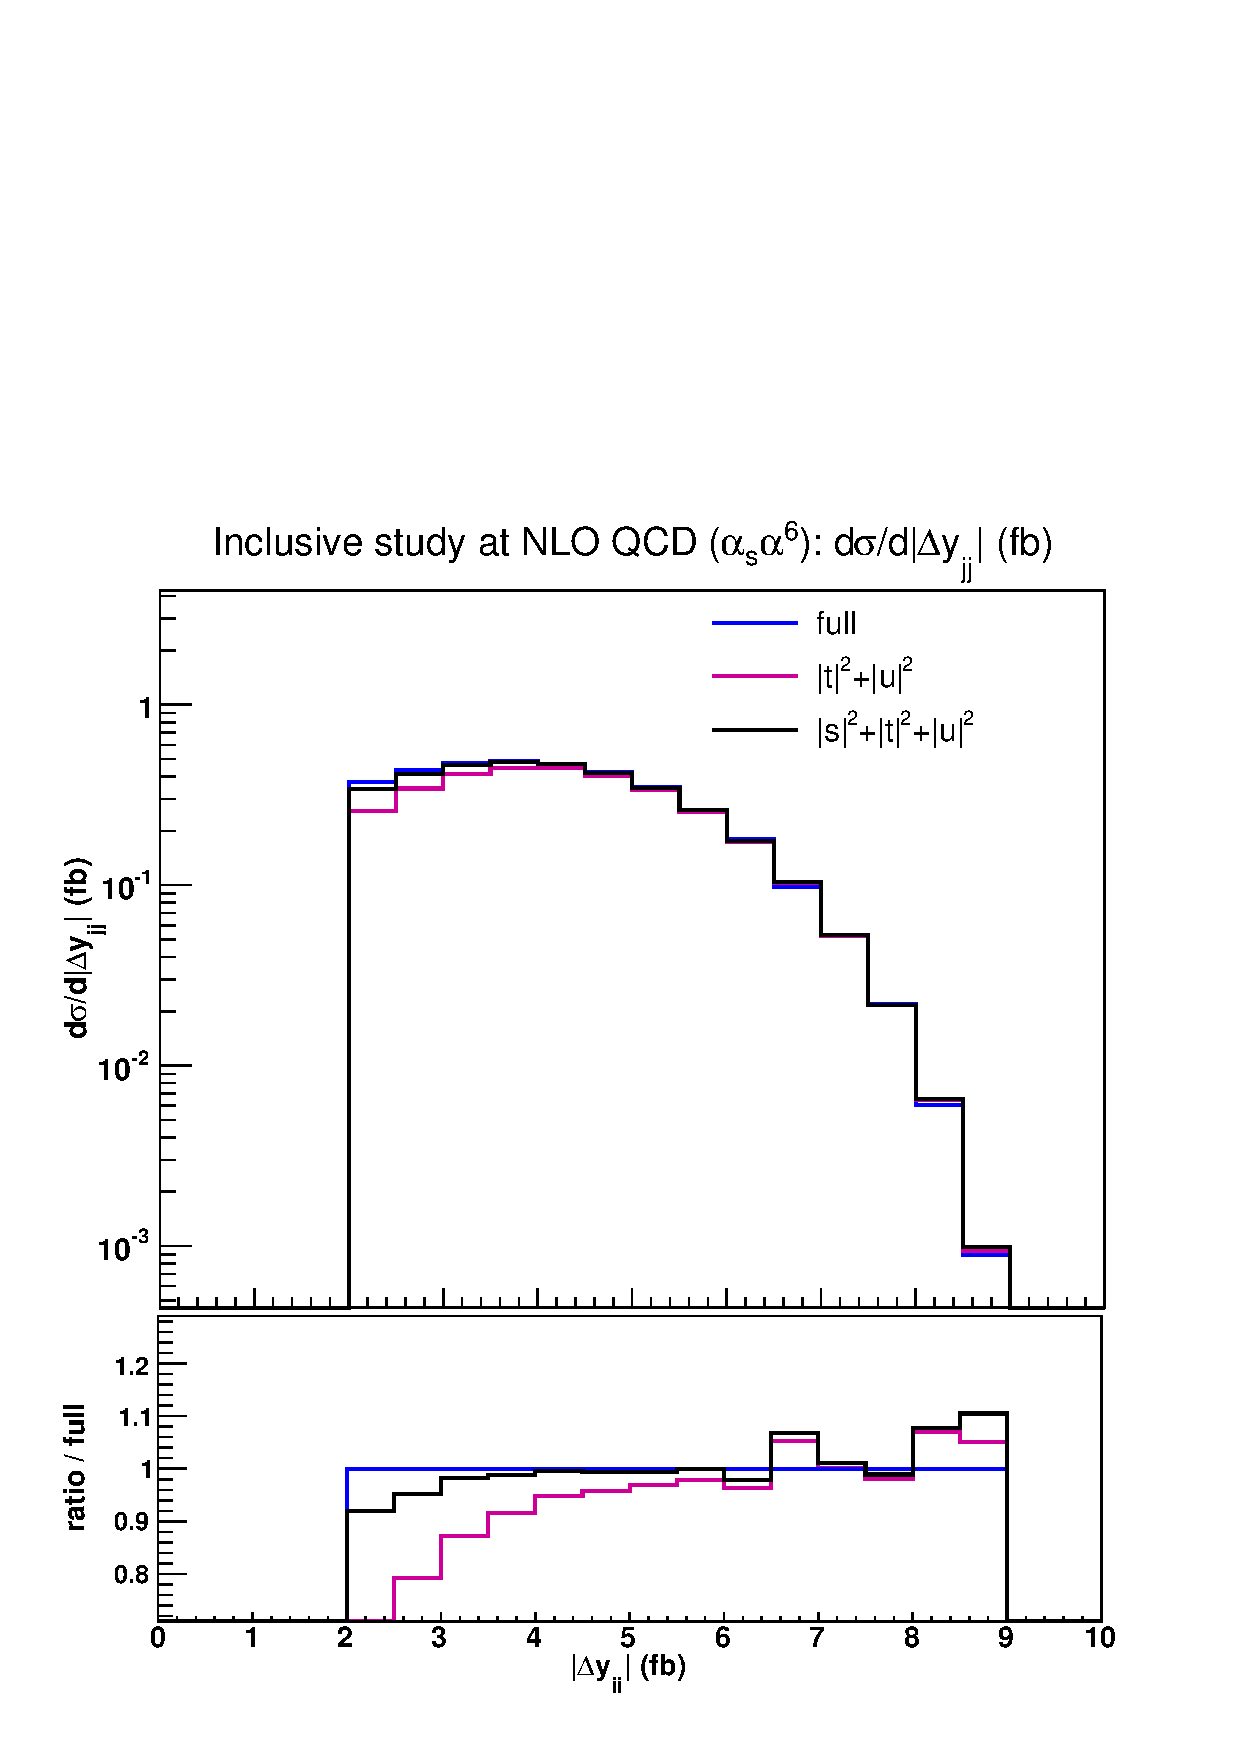
\includegraphics[scale=0.35]{figures/scanfigures/dyjj_nlo.pdf}}
\caption{
Differential distributions in the di-jet invariant mass (left) and the rapidity-separation of the two tagging jets (right) at NLO QCD \emph{i.e.}\ at order $\mathcal{O}(\alphas\alpha^6)$ for the full computation and two approximations.
The upper plots provide the absolute value for each prediction while the lower plots presents all predictions normalised to {\sc MoCaNLO}+{\sc Recola} which is one of the full predictions.
In addition to the cuts of Sec.~\ref{subsec:inputpar}, the VBS cuts take the values $m_{\Pj\Pj}>200 \GeV$ and $|\Delta y_{\Pj\Pj}|>2$.} 
\label{fig:mjjdyjj_1d_1}
\end{figure*}


\begin{figure*}[hbt]
\centering
{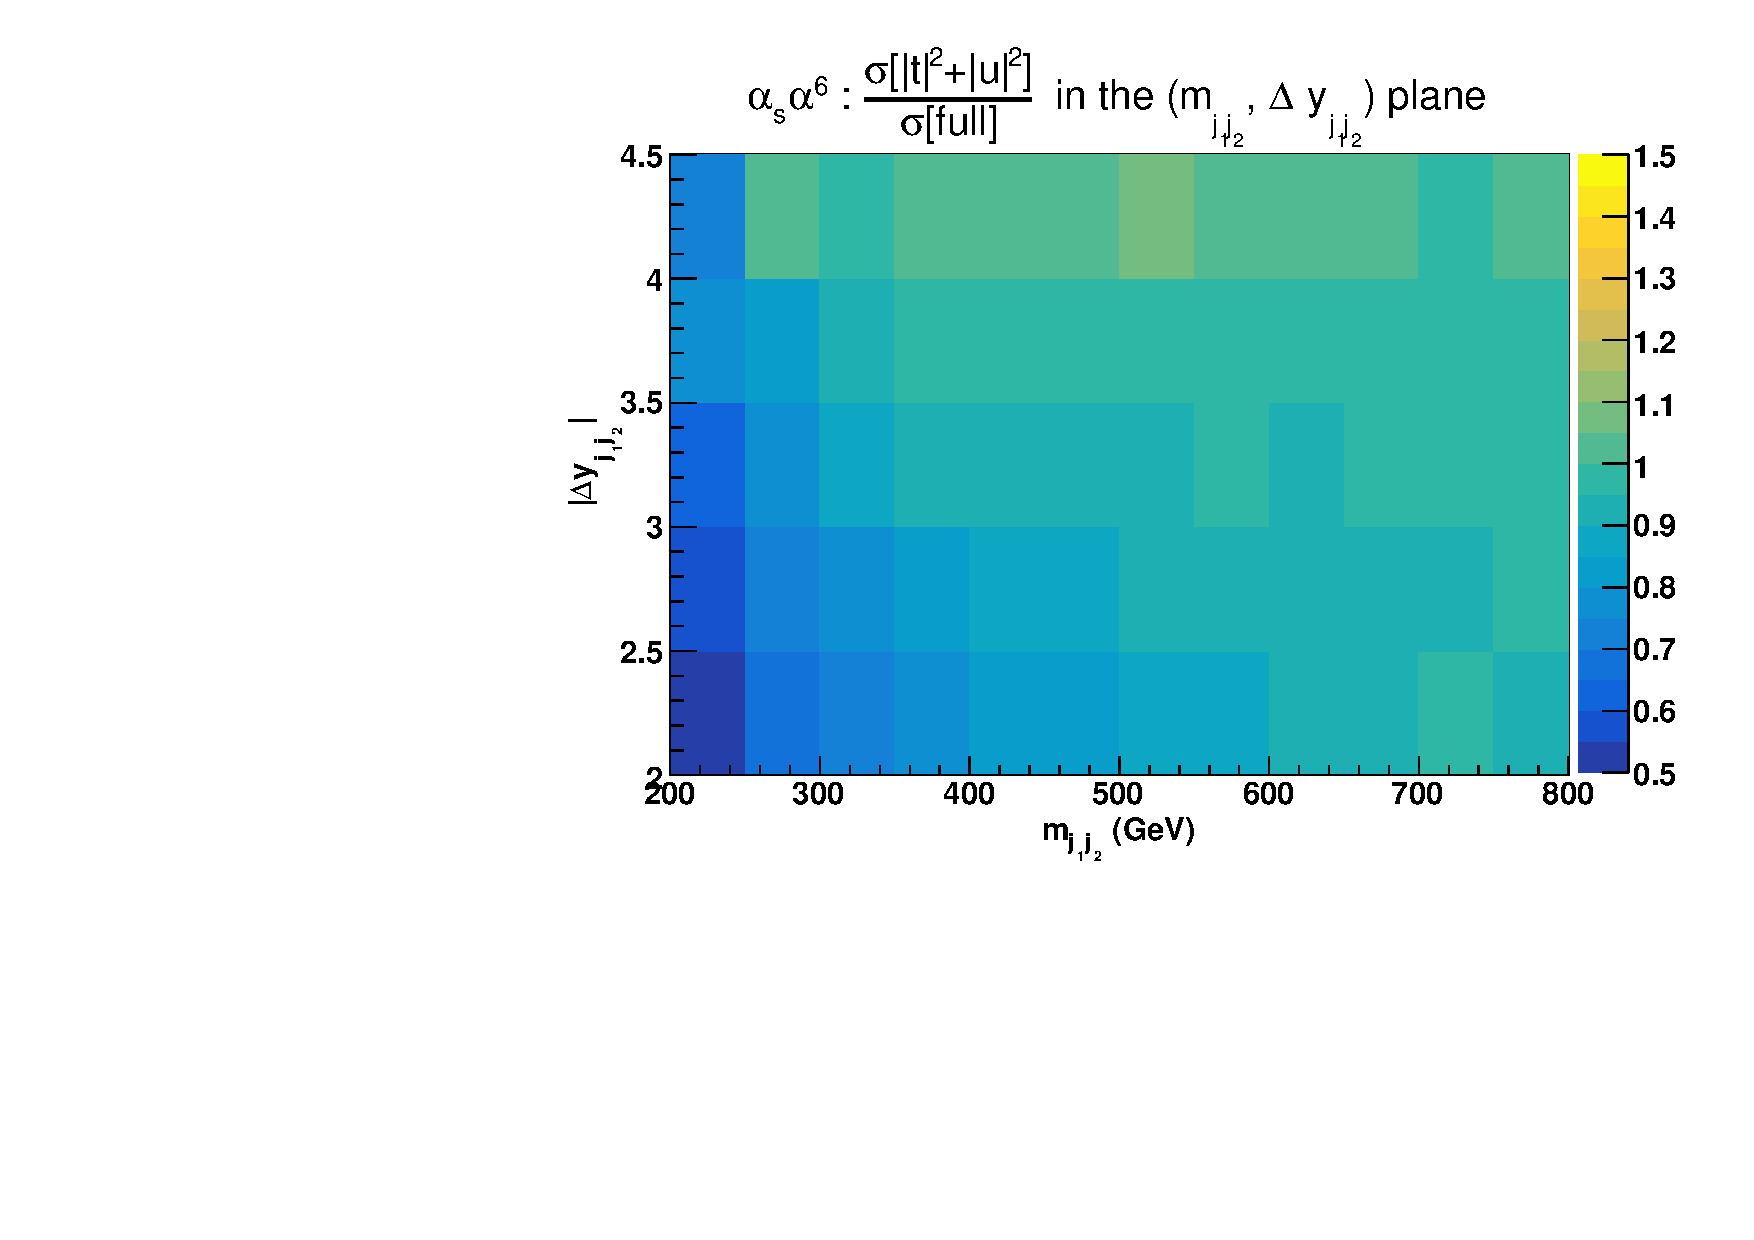
\includegraphics[scale=0.395]{figures/scanfigures/a6as_vbfnloVSrecola_tu.pdf}}
{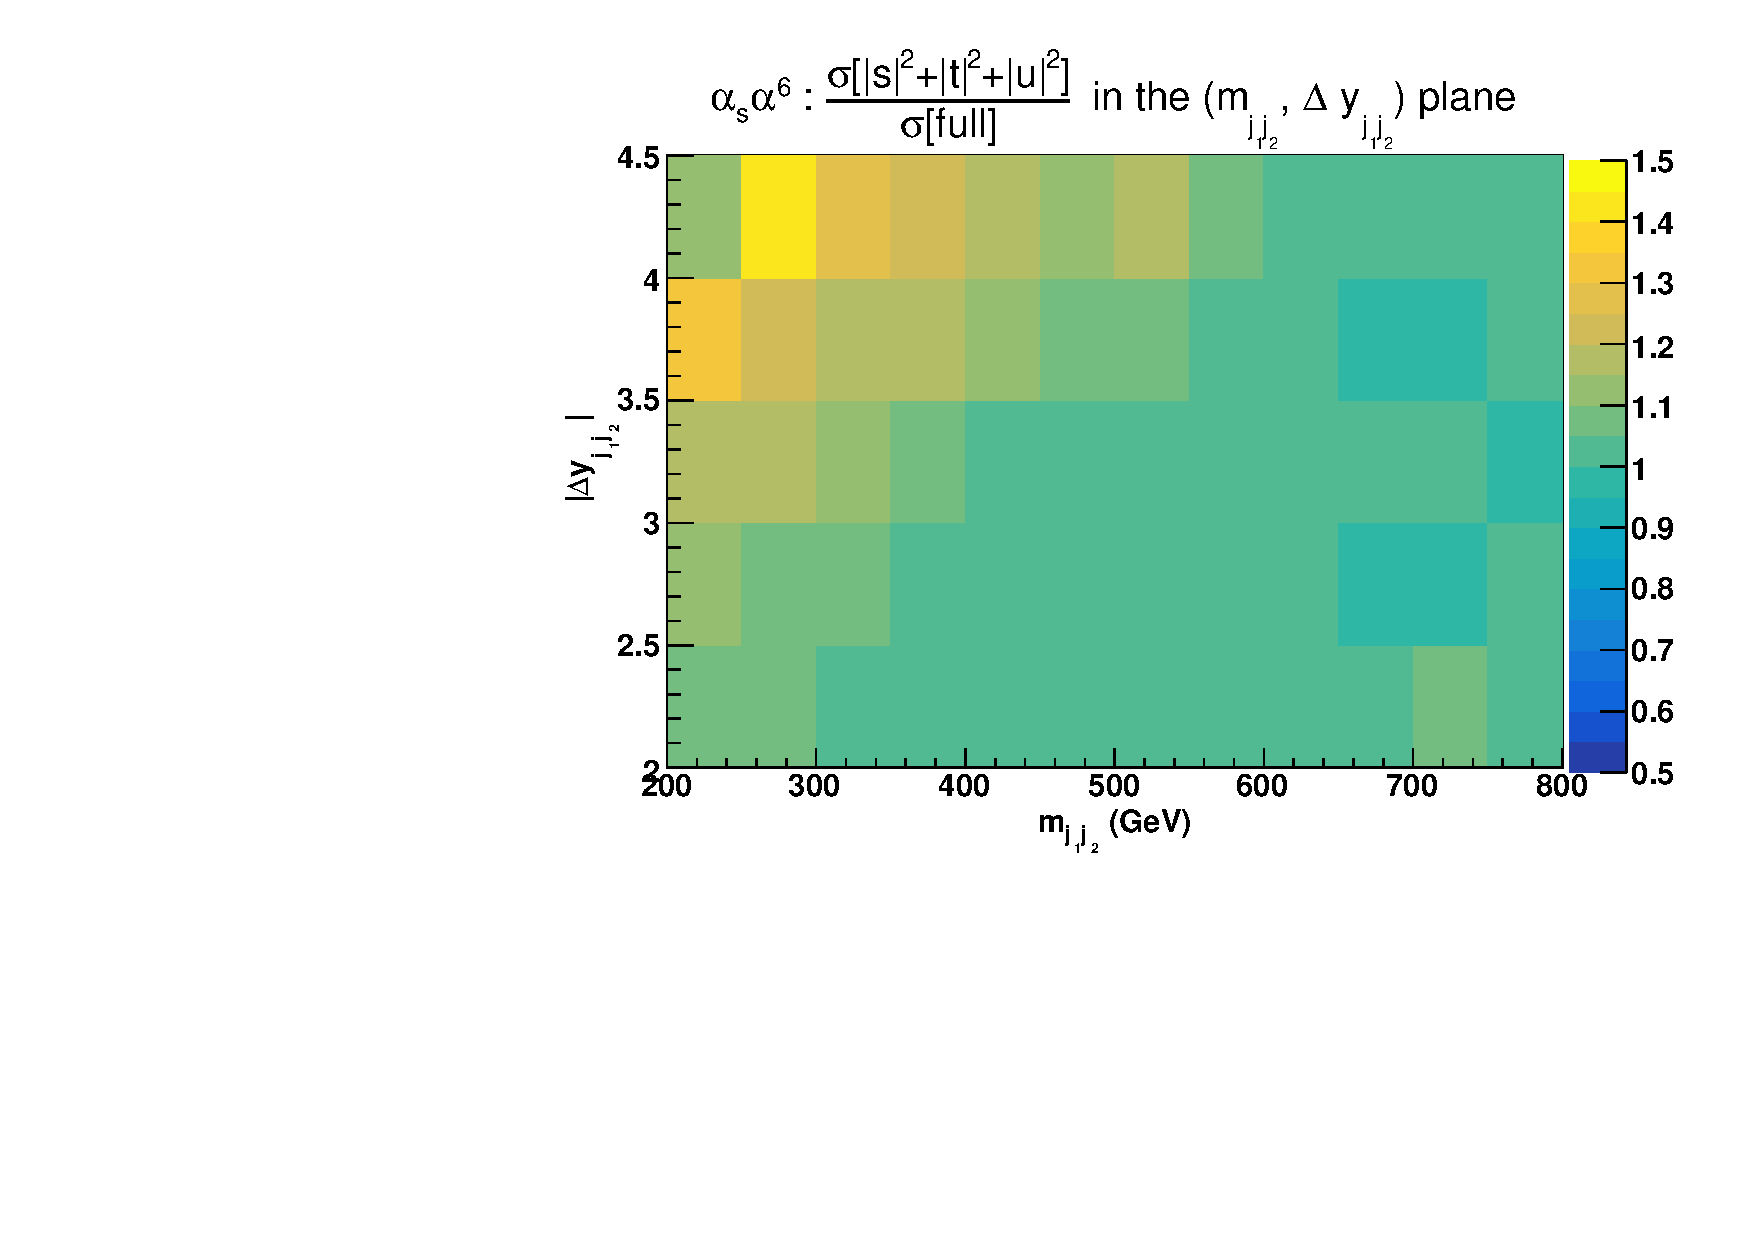
\includegraphics[scale=0.395]{figures/scanfigures/a6as_vbfnloVSrecola_stu.pdf}}
\caption{Ratios of double-differential distributions in the variables $m_{\Pj\Pj}$ and $|\Delta y_{\Pj\Pj}|$ at NLO QCD \emph{i.e.}\ at order $\mathcal{O}(\alphas\alpha^6)$ for the VBS approximation over the full computation.
Ratio of approximated squared amplitudes over the full matrix element.
The approximated squared amplitudes are computed as $|\mathcal{A}|^2 \sim |t|^2+|u|^2$ (left) and $|\mathcal{A}|^2 \sim |s|^2+|t|^2+|u|^2$ (right)
In addition to the cuts of Sec.~\ref{subsec:inputpar}, the VBS cuts take the values $m_{\Pj\Pj}>200 \GeV$ and $|\Delta y_{\Pj\Pj}|>2$.}
\label{fig:ratio2d_NLO}
\end{figure*}
%
% \begin{figure}[hbt]
% \centering
% {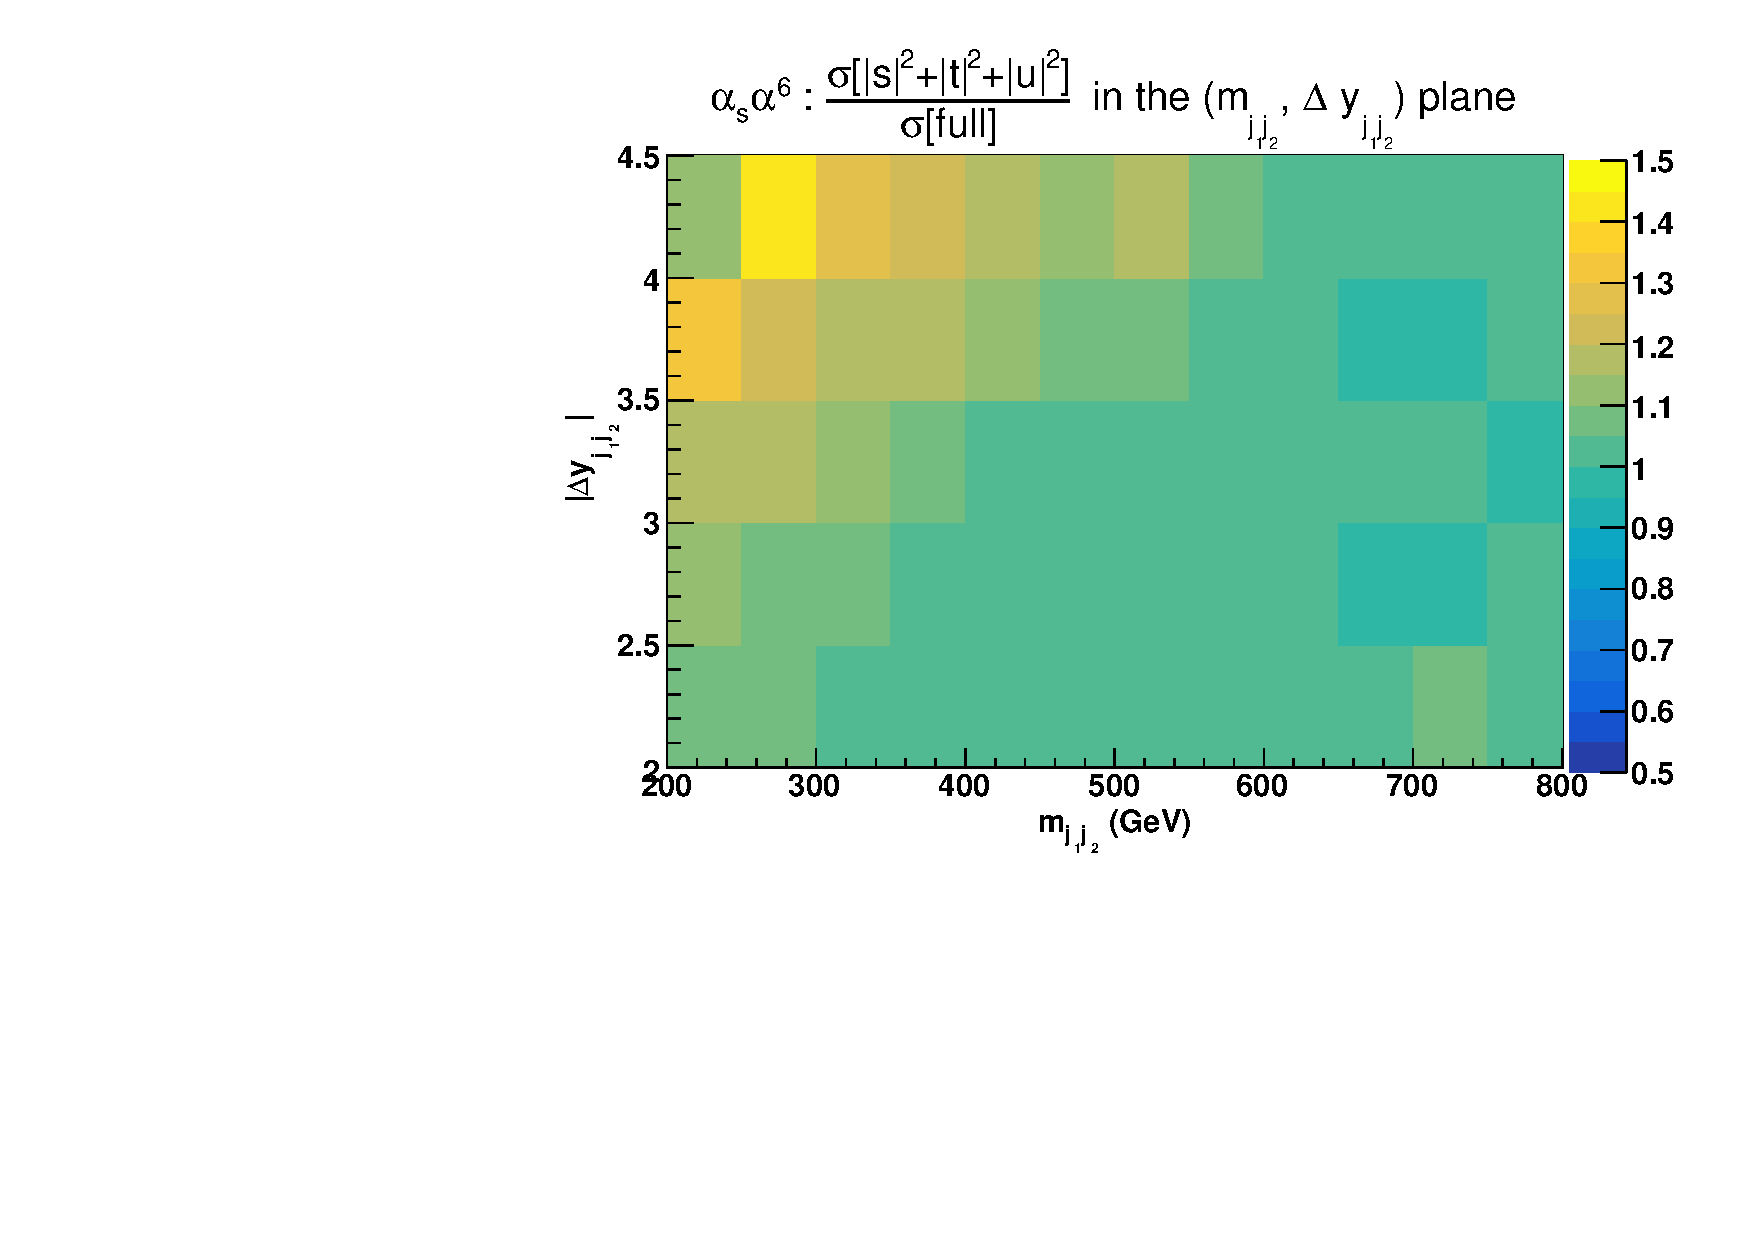
\includegraphics[scale=0.39]{figures/scanfigures/a6as_vbfnloVSrecola_stu.pdf}}
% \caption{Ratio of cross sections (fb) per bin in the plan $\left(m_{\Pj\Pj}, |\Delta y_{\Pj\Pj}| \right)$ at NLO QCD \emph{i.e.}\ at order $\mathcal{O}(\alphas\alpha^6)$ for the VBS approximation with $s$-channel contributions over the full computation.
% In addition to the cuts of Sec.~\ref{subsec:inputpar}, the VBS cuts take the values: $m_{\Pj\Pj}>200 \GeV$ and $|\Delta y_{\Pj\Pj}|>2$.}
% \label{fig:mjjdyjj_2d_NLO}
% \end{figure}

As expected, in the low invariant-mass and low rapidity-separation region of the jet pair ($200 \GeV < m_{\Pj\Pj} < 500 \GeV$, $2<|\Delta y_{\Pj\Pj}|<2.5$) the VBS approximation fails significantly (up to $30\%$ discrepancy).
Including the $s$-channel contributions leads to a difference of $5\%$.
However, in the region of large di-jet invariant mass and low rapidity separation of the jets, the $|s|^2+|t|^2+|u|^2$ approximation overshoot the full computation by $40\%$.
On the other hand, in the typical VBS region, the VBS approximation shows a good agreement with the full computation as documented in details in Sec.~\ref{sec:fidNLO}

% However, the positive discrepancy shown in the low $m_{\Pj\Pj}$ region (black curve on the upper plots of Fig.~\ref{fig:mjjdyjj_1d_1}) can be traced back to the low $m_{\Pj\Pj}$, large $\Delta y_{\Pj\Pj}$ region of Fig.~\ref{fig:ratio2d_NLO}.
% In this region, the two leading jets have soft transverse momenta, according to the following low-angle approximation
% 
% \begin{equation}
% \begin{split}
% m_{\Pj_i\Pj_j}^2 &= 2\,\ptsub{\Pj_i}\ptsub{\Pj_j}\,(\cosh \Delta y_{\Pj_i\Pj_j} - \cos \Delta\phi_{\Pj_i\Pj_j}) \\
% &\approx 2\,\ptsub{\Pj_i}\ptsub{\Pj_j}\,\cosh \Delta y_{\Pj_i\Pj_j} \,\,.
% \end{split}
% \end{equation}

% The same positive discrepancy for the $|s|^2 + |t|^2 + |u|^2$ approximation, can be seen in the low transverse-momentum region of the leading jet in the upper plot of Fig.~\ref{fig:mjjdyjj_1d_2}.
% In the large invariant mass--small rapidity separation region of Fig.~\ref{fig:ratio2d_NLO}, discrepancies at the level of $15\%$ are present.
% This can be traced back to the large $\pt$ and central rapidity region of the leading jets kinematics, shown in Fig.~\ref{fig:mjjdyjj_1d_2}.
% For such distributions, despite the $s$-channel inclusion, the discrepancy between the approximated and full result is about $5-10\%$.
% In the VBS signal-region the VBS approximation shows a good agreement with the full calculation as documented in details below.

In Fig.~\ref{fig:mjjdyjj_1d_2}, the distributions in the transverse momentum of the hardest jet and its rapidity are shown.
At low transverse momentum, $|t|^2+|u|^2$ and $|s|^2+|t|^2+|u|^2$ approximations are lower and higher than the full computation by about $20\%$, respectively.
At high transverse momentum, they have a similar behaviour.
They both diverge from the full computation towards larger transverse momentum to reach about $10\%$ at $1000\GeV$.
Regarding the rapidity of the hardest jet, the two approximations have opposite behaviours.
In the central region, the $|t|^2+|u|^2$ approximation differs by $12\%$ with respect to the full computation while the $|s|^2+|t|^2+|u|^2$ one is good within $5\%$.
In the peripheral region, the $|t|^2+|u|^2$ approximation is rather close to the full computation ($5\%$) while the $|s|^2+|t|^2+|u|^2$ one differs by $10\%$.

\begin{figure*}[hbt]
\centering
{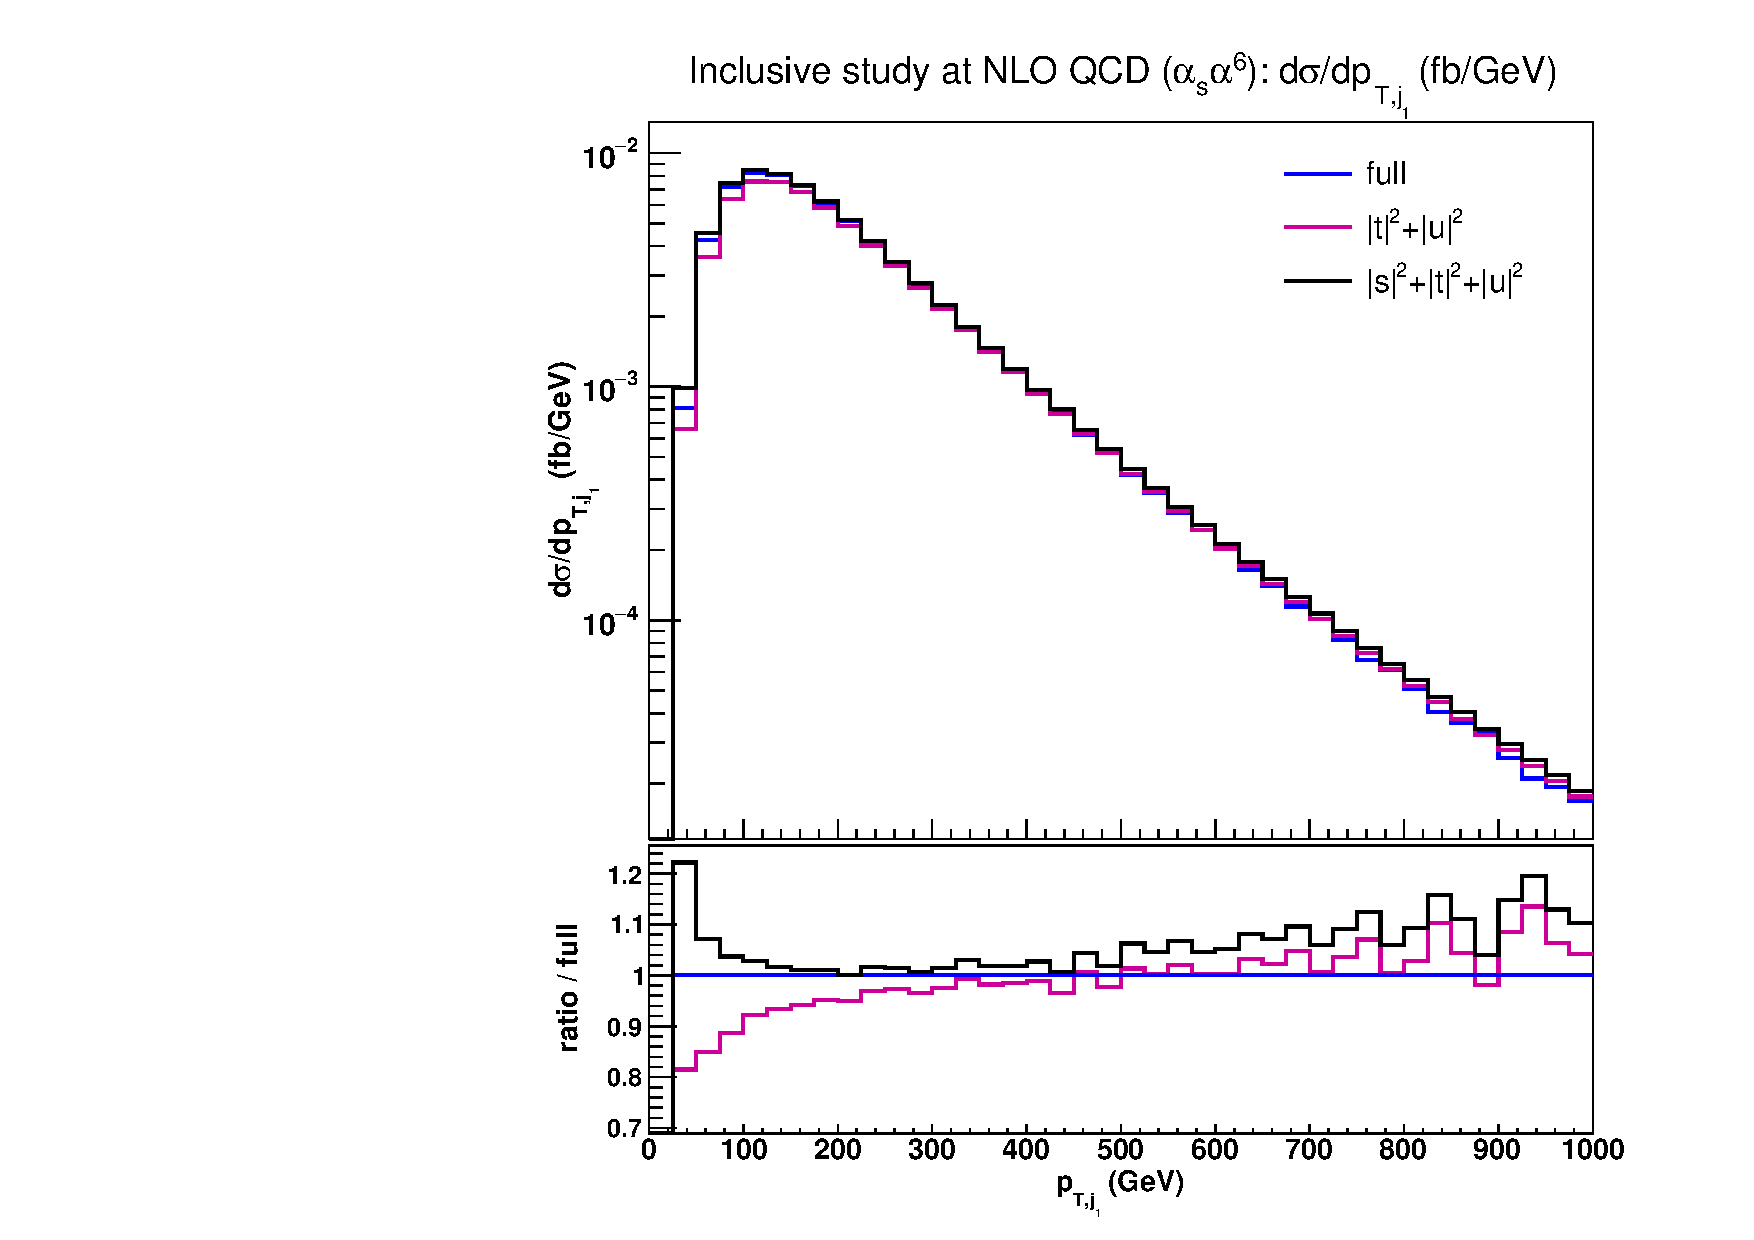
\includegraphics[scale=0.35]{figures/scanfigures/ptj1_nlo.pdf}}
{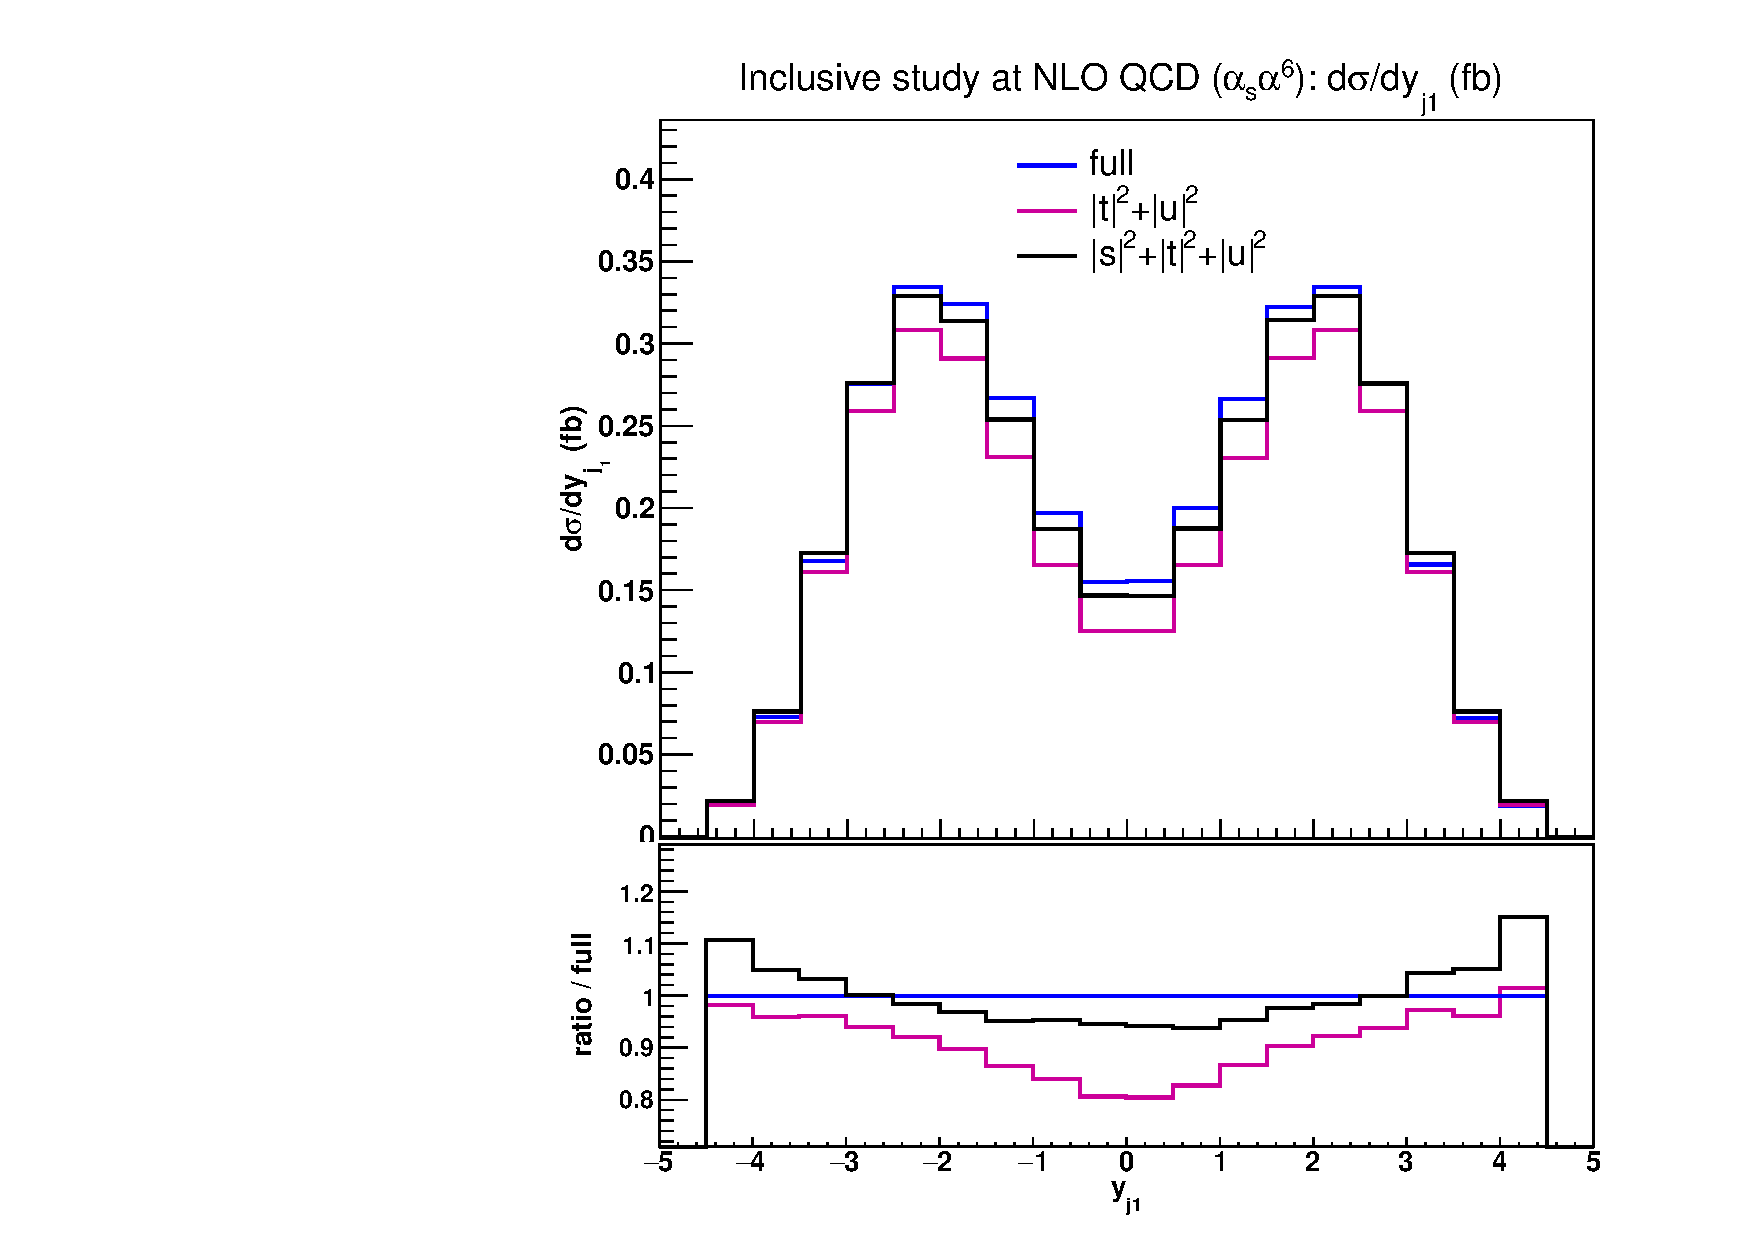
\includegraphics[scale=0.35]{figures/scanfigures/yj1_nlo.pdf}}
\caption{Differential distributions in the transverse momentum (left) and rapidity of the hardest tagging jet (right) at NLO QCD \emph{i.e.}\ at order $\mathcal{O}(\alphas\alpha^6)$ for the full computation and two approximations.
The upper plots provide the absolute value for each prediction while the lower plots presents all predictions normalised to {\sc MoCaNLO}+{\sc Recola} which is one of the full predictions.
In addition to the cuts of Sec.~\ref{subsec:inputpar}, the VBS cuts take the values $m_{\Pj\Pj}>200 \GeV$ and $|\Delta y_{\Pj\Pj}|>2$.} 
\label{fig:mjjdyjj_1d_2}
\end{figure*}

Concerning leptonic observables, we show in Fig.~\ref{fig:mjjdyjj_1d_3} the distributions in the di-lepton invariant mass and in the Zeppenfeld variable of the electron, defined as
%
\begin{equation}
%  z_{\Pe^+} = \frac{y_{\Pe^+}-\frac{y_{\Pj_1}+y_{\Pj2}}2}{|y_{\Pj_1}-y_{\Pj_2}|} \,.
  z_{\Pe^+} = \frac{y_{\Pe^+}-\frac{y_{\Pj_1}+y_{\Pj2}}2}{|\Delta y_{jj}|} \,.
  \label{eq:Zeppenfeld}
\end{equation}
%
Analogous definitions will later also be used for the Zeppenfeld variable of the muon and of the third jet.
%
\begin{figure*}[hbt]
\centering
{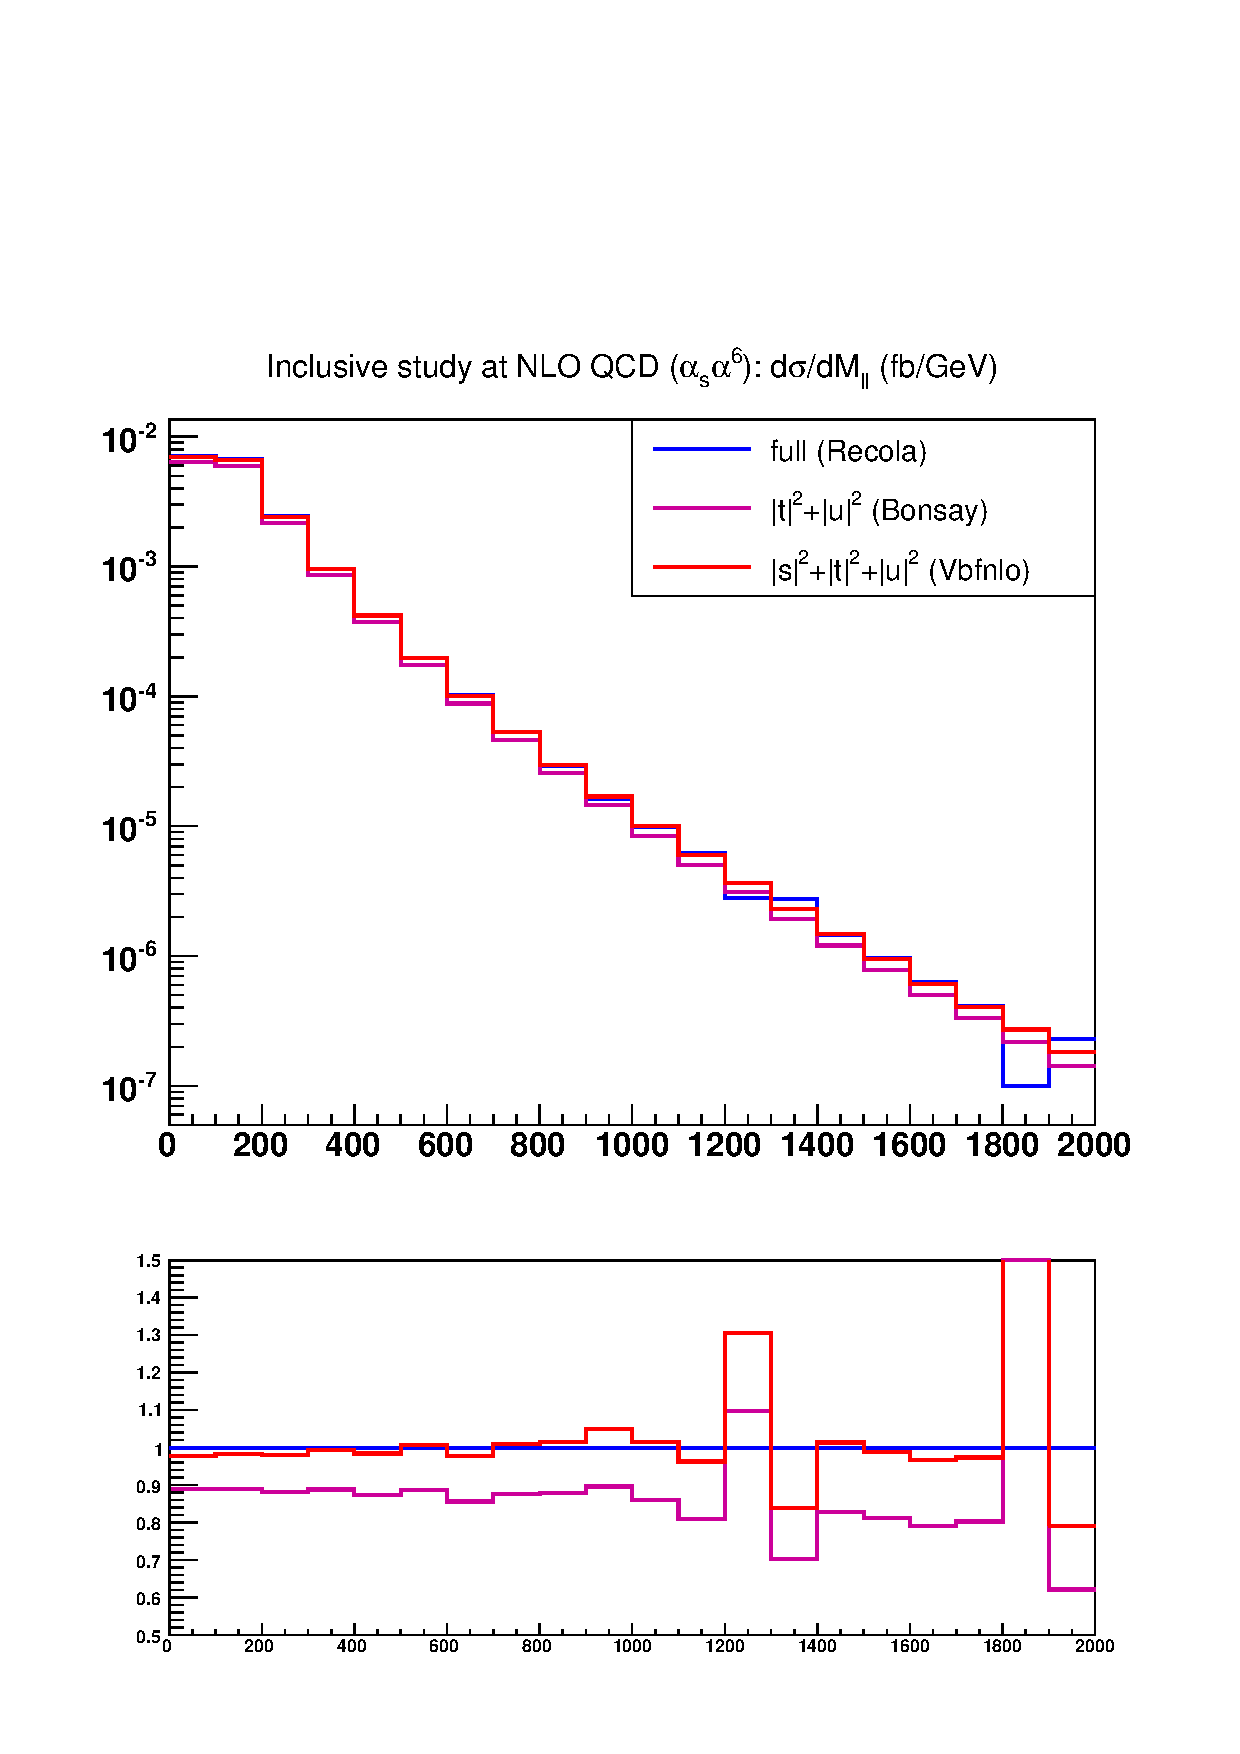
\includegraphics[scale=0.35]{figures/scanfigures/mll_nlo.pdf}}
{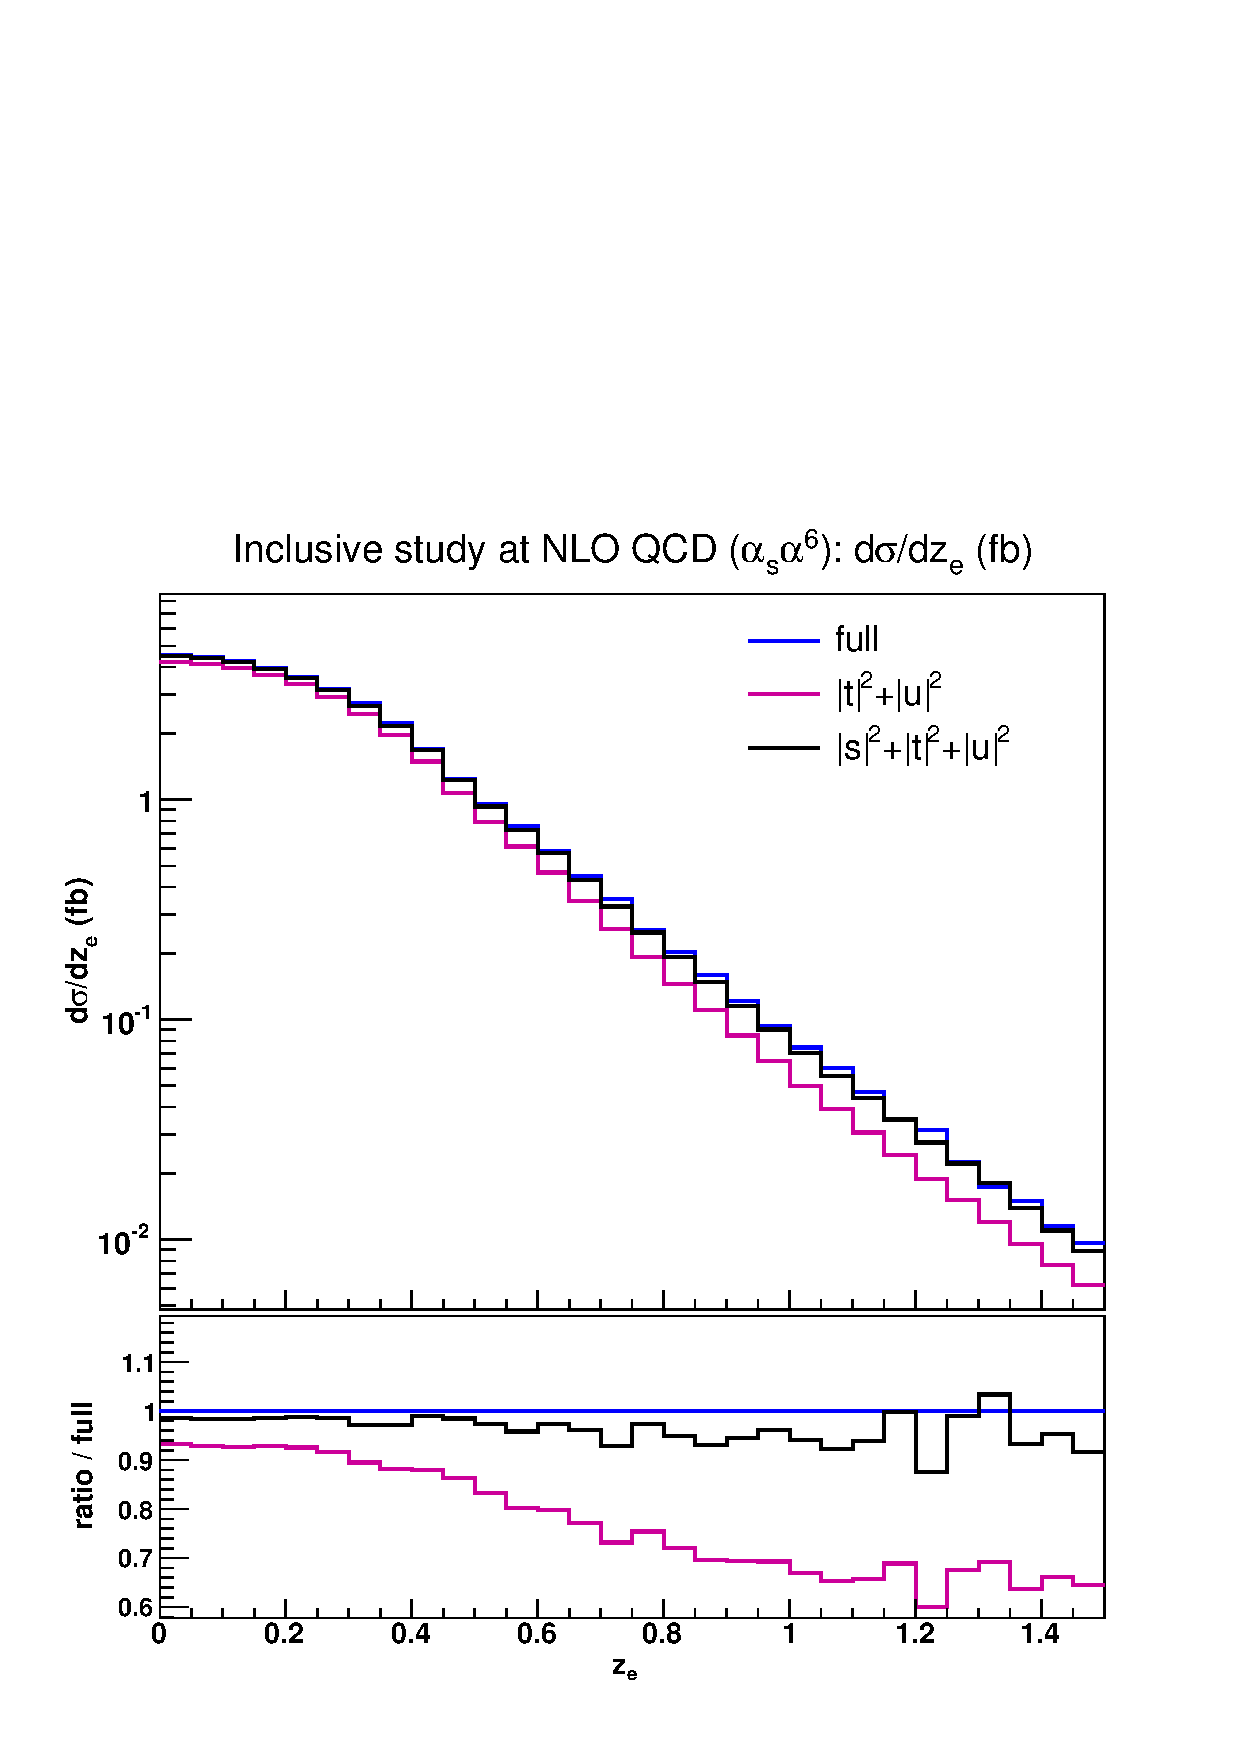
\includegraphics[scale=0.35]{figures/scanfigures/zel_nlo.pdf}}
\caption{Differential distributions in the lepton-lepton invariant mass (left) and the electron Zeppenfeld variable (right) at NLO QCD \emph{i.e.}\ at order $\mathcal{O}(\alphas\alpha^6)$ for the full computation and two approximations.
The upper plots provide the absolute value for each prediction while the lower plots presents all predictions normalised to {\sc MoCaNLO}+{\sc Recola} which is one of the full predictions.
In addition to the cuts of Sec.~\ref{subsec:inputpar}, the VBS cuts take the values $m_{\Pj\Pj}>200 \GeV$ and $|\Delta y_{\Pj\Pj}|>2$.} 
\label{fig:mjjdyjj_1d_3}
\end{figure*}
%
The $|s|^2+|t|^2+|u|^2$ predictions for $m-{\rm e^+\mu^+}$ agrees rather well with the full curve, obtained from {\sc MoCa\-NLO+Recola}.
The prediction from {\sc Bonsay} is about $10\%$ lower around $1000 \GeV$.
% ; this discrepancy reaches about $20\%$ in the very high mass region. 
%The discrepancies are roughly constant over the whole spectrum.
% Instead, the right panel of Fig.~\ref{fig:mjjdyjj_1d_3} clearly shows that
The Zeppenfeld variable of the positron $z_e$ is more strongly affected by the exclusion of $s$-channels.
% with increasing negative discrepancy with respect to the full result at large values (up to $30\%$ for $z_{e^+}>1.2$).
% Including $s$-channels makes this discrepancy become positive, but smaller than $10\%$ over the whole spectrum.
% The muon observable $z_{\mu}$ behaves identically to the electron one, $z_e$.
For increasing $z_{\rm e}$, the $|t|^2+|u|^2$ approximation diverges from the full computation to reach about a $25\%$ difference  at $1.5$.
On the other hand, including $s$-channel contributions leads to a better approximation, staying within $10\%$ difference over the whole range.

In conclusion, both the loose minimum di-jet invariant mass cut and the inclusion of QCD radiative correction make the $s$-channel contributions less suppressed than at LO, making their inclusion mandatory, in order to provide trustworthy predictions at NLO accuracy.
% Nevertheless, interferences and non-factorizable QCD corrections should be included to reduce the discrepancies down to about $1\%$, mainly in inclusive analyses.
In the inclusive region studied here, neglecting $s$-channel, non-factorisable corrections, and electroweak corrections can lead to discrepancies of up to $30\%$ with respect to the full computation.
Nevertheless, the VBS approximation at NLO provides a good approximation of full calculations in the kinematic region where VBS contributions are dominant ($m_{\Pj\Pj} \gtrsim 500 \GeV$, $|\Delta y_{\Pj\Pj}| \gtrsim 2.5$), for both total cross section and differential distributions.
This more exclusive region is studied in more details in the next section.

\subsection{Comparison in the fiducial region}

Cross secitons at NLO

\begin{table}[h!]
    \centering
    \begin{tabular}{c|c|c|c}
        Code  &  $\sigma[\rm{fb}]$  \\
        \hline
        \hline
        {\sc Bonsay}  &  $X \pm 0.0009$  \\
        {\sc MG5\_aMC}&  $X  \pm 0.003$  \\
        {\sc MoCaNLO+Recola}  &  $ 1.382 \pm 0.002$ \\
        {\sc POWHEG}  &  $1.3556 \pm 0.0009$  \\
        {\sc VBFNLO}  &  $1.3916 \pm 0.0001$  \\
    \end{tabular}
    \caption{\label{tab:wg1_NLOrates} Rates at NLO-QCD accuracy within VBS cuts obtained with the different codes used in this comparison, 
    for the ${\rm p}{\rm p}\to\mu^+\nu_\mu{\rm e}^+\nu_{\rm e}{\rm j}{\rm j}$ process.}
\end{table}
At NLO, rates show slightly larger discrepancies, as it can be observed in Tab.~\ref{tab:wg1_NLOrates}. This is most likely due to low dijet invariant-mass configurations, where
$s-$channel diagrams and interferences are less suppressed than at LO, because of the presence of extra QCD radiation.

In Figs.~\ref{fig:distNLO1}--\ref{fig:distNLO3}, several differential distributions are shown.
All these predictions are performed at NLO accuracy at the order $\mathcal{O}(\alphas\alpha^6)$.
In the upper panel, the absolute predictions are shown while in the lower panel, the ratio with respect to the full predictions are displayed.
The band corresponds to a seven-points variation of the factorisation and renormalisation scales.

We start with Fig.~\ref{fig:distNLO1} which displays the invariant mass (left) and the rapidity separation (right) of the two tagging jets.
For high invariant mass, all predictions agree rather well.
On the other hand, for low invariant mass, the hierarchy present at the level of the cross section is here reproduced.
The VBS-approximated predictions ({\sc Bonsay} and {\sc Powheg-Box}) are lower than the full calculation ({\sc MoCaNLO}+{\sc Recola}).
The full calculation is rather well approximated by the hybrid VBS approximation implemented in {\sc MG5\_aMC}.
Finally, {\sc VBFNLO} which includes also $s$-channel contributions provides larger predictions at low invariant mass.
For the rapidity difference between the two tagging jets, the hierarchy between the predictions is rather similar.
Therefore, depending on the approximation used, it can vary by $\pm7\%$ and $\pm4\%$ with respect to the full computation at low invariant mass and low rapidity difference for the tagging jets, respectively

 \begin{figure*}[hbt!]
   \centering
   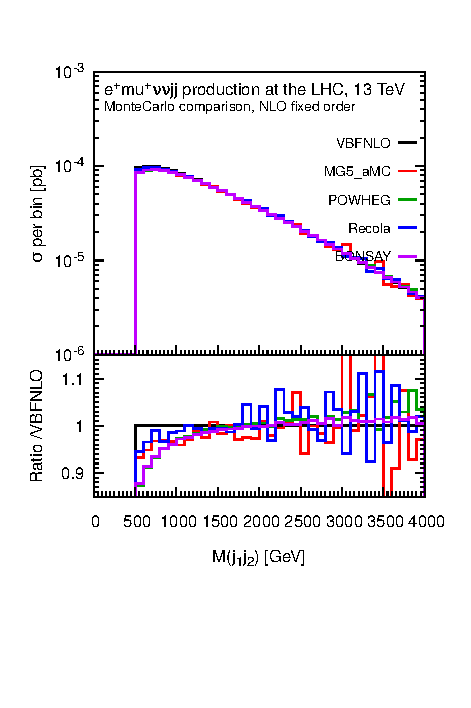
\includegraphics[width=0.4\textwidth,angle=0,clip=true,trim={0.4cm 2cm 0.cm 1.cm}]{figures/NLO/mjj_NLO.pdf}
   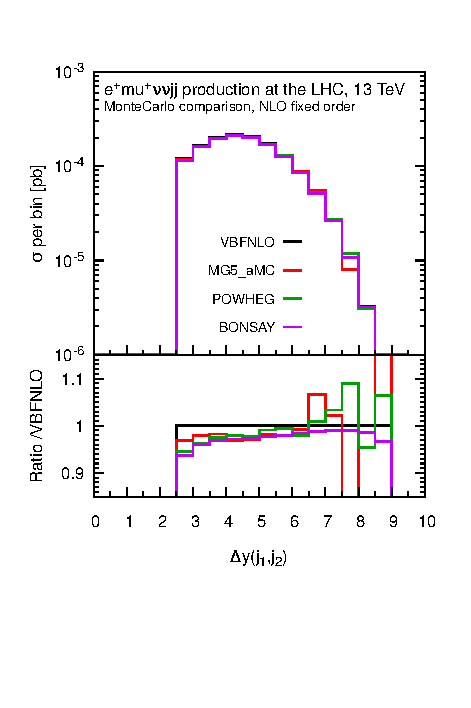
\includegraphics[width=0.4\textwidth,angle=0,clip=true,trim={0.4cm 2cm 0.cm 1.cm}]{figures/NLO/dyj1j2_NLO.pdf}
\caption{\label{fig:distNLO1} Differential distributions in the invariant mass (left) and rapidity difference of the two tagging jets (right).
The LHC process considered is ${\rm p}{\rm p}\to\mu^+\nu_\mu{\rm e}^+\nu_{\rm e}{\rm j}{\rm j}$ at NLO accuracy at order $\mathcal{O}(\alpha_{\rm s}\alpha^6)$.
The description of the different programs used can be found in Sec.~\ref{subsec:codedescr}.
The upper plots provide the absolute value for each prediction while the lower plots present all predictions normalised to {\sc MoCaNLO}+{\sc Recola} which is the full predictions.
The band corresponds to a seven-points scale variation of the renormalisation and factorisation scale.
The predictions are obtained in the fiducial region described in Sec.~\ref{subsec:inputpar}.
}
\end{figure*}

Concerning the transverse momentum (left) and rapidity (right) of the hardest jet shown in Fig.~\ref{fig:distNLO2}, the situation is rather different.
While {\sc MG5\_aMC} is very close to the full prediction for low transverse momentum, it departs from it 
at larger transverse momentum by about $10\%$.
This is in contrast with the VBS-approximated predictions such as {\sc Bonsay}, {\sc Powheg}, and {\sc VBFNLO} which are lower than the full computation at low transverse momentum and higher for larger transverse momentum.
The difference at high transverse momentum between the latter predictions and the full computation can be attributed to EW Sudakov logarithms that become large in this phase-space region.
While, the predictions of {\sc Bonsay} and {\sc Powheg} are rather close over the whole range, the one of {\sc VBFNLO} is very different at low transverse momentum where it is even higher than the full computation.
We note that for the transverse momentum of the second hardest jet, the predictions from {\sc MG5\_aMC} are in good agreement with the other VBS-approximated predictions.
% Finally, {\sc VBFNLO} predicts higher rates over the whole range apart from around $200\GeV$ where it is in perfect agreement with the complete calculation.
Concerning the rapidity of the hardest jet, {\sc VBFNLO} is in good agreement with {\sc MoCaNLO}+{\sc Recola} in the rapidity range $|y_{j_1}| < 3$.
For larger rapidity, the other codes constitute a better description of the full process at order $\mathcal{O}(\alpha_{\rm s}\alpha^6)$.

 \begin{figure*}[hbt!]
   \centering
   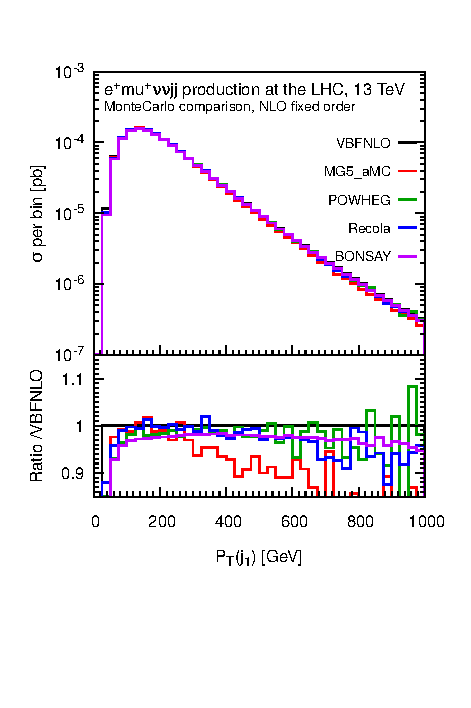
\includegraphics[width=0.4\textwidth,angle=0,clip=true,trim={0.4cm 2cm 0.cm 1.cm}]{figures/NLO/ptj1_NLO.pdf}
   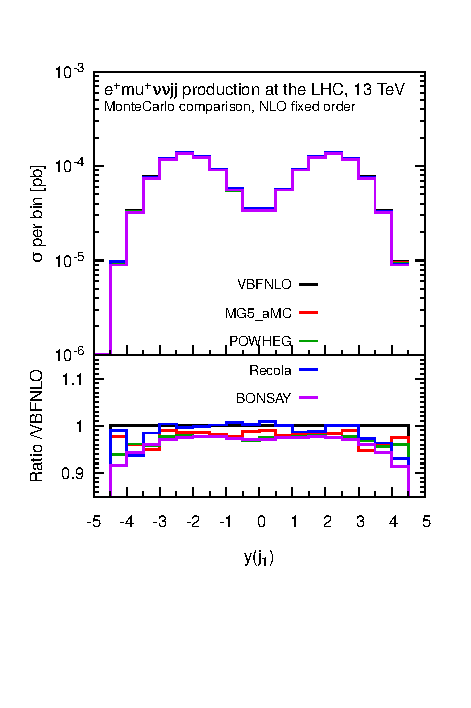
\includegraphics[width=0.4\textwidth,angle=0,clip=true,trim={0.4cm 2cm 0.cm 1.cm}]{figures/NLO/yj1_NLO.pdf}
\caption{\label{fig:distNLO2} Differential distributions in the transverse momentum (left) and rapidity of the hardest jet (right).
The LHC process considered is ${\rm p}{\rm p}\to\mu^+\nu_\mu{\rm e}^+\nu_{\rm e}{\rm j}{\rm j}$ at NLO accuracy at order $\mathcal{O}(\alpha_{\rm s}\alpha^6)$.
The description of the different programs used can be found in Sec.~\ref{subsec:codedescr}.
The upper plots provide the absolute value for each prediction while the lower plots present all predictions normalised to {\sc MoCaNLO}+{\sc Recola} which is the full predictions.
The band corresponds to a seven-points scale variation of the renormalisation and factorisation scale.
The predictions are obtained in the fiducial region described in Sec.~\ref{subsec:inputpar}.
}
\end{figure*}

The last set of differential distributions is the invariant mass of the two charged lepton (left) and the Zeppenfeld variable for the anti-muon (right).
Concerning the comparison of the predictions, both distributions display a rather similar behaviour.
Indeed, the hierarchy mentioned previously is here respected and enhanced towards high invariant mass or high Zeppenfeld variable.
The predictions of {\sc MoCaNLO}+{\sc Recola} and {\sc VBFNLO} are in rather good agreement for both distributions for the kinematic range displayed here.
The other three VBS approximations are close to each other within few per cent.

 \begin{figure*}[hbt!]
   \centering
   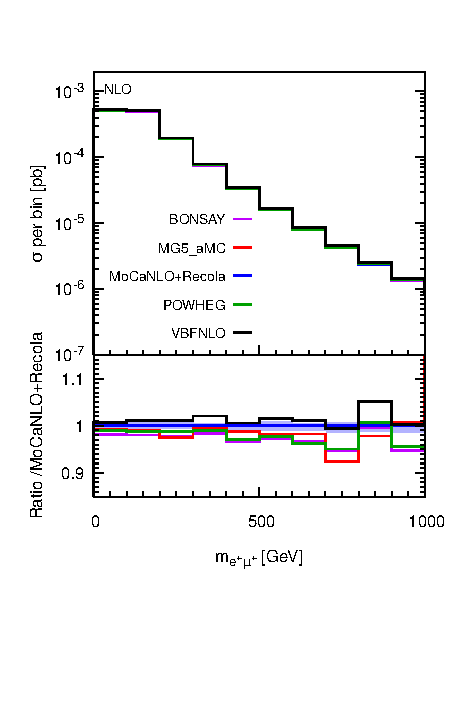
\includegraphics[width=0.4\textwidth,angle=0,clip=true,trim={0.4cm 2cm 0.cm 1.cm}]{figures/NLO/mll_NLO.pdf}
   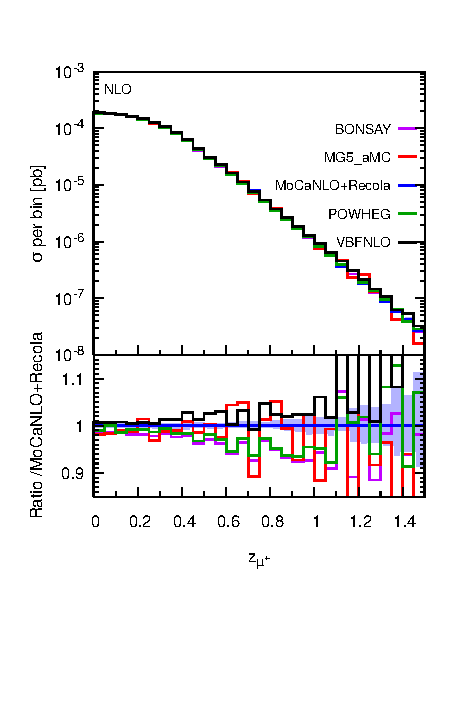
\includegraphics[width=0.4\textwidth,angle=0,clip=true,trim={0.4cm 2cm 0.cm 1.cm}]{figures/NLO/zmu_NLO.pdf}
\caption{\label{fig:distNLO3} Differential distributions in the invariant mass of the two charged leptons (left) and Zeppenfeld variable for the muon (right).
The LHC process considered is ${\rm p}{\rm p}\to\mu^+\nu_\mu{\rm e}^+\nu_{\rm e}{\rm j}{\rm j}$ at NLO accuracy at order $\mathcal{O}(\alpha_{\rm s}\alpha^6)$.
The description of the different programs used can be found in Sec.~\ref{subsec:codedescr}.
The upper plots provide the absolute value for each prediction while the lower plots present all predictions normalised to {\sc MoCaNLO}+{\sc Recola} which is the full predictions.
The band corresponds to a seven-points scale variation of the renormalisation and factorisation scale.
The predictions are obtained in the fiducial region described in Sec.~\ref{subsec:inputpar}.
}
\end{figure*}

In the end, the quality of the VBS approximations is good up to $10\%$ in the fiducial region.
These differences are larger than those at LO.

The contributions from the $s$-channel amplitude can be sizeable especially at low invariant mass for the two tagging jets (comparing the predictions of {\sc VBFNLO} against the ones of {\sc Bonsay} and {\sc Powheg}).
This can be explained by the fact that $s$-channel contributions are less suppressed at NLO.
In the real, an extra gluon-jet can be radiated from any of the charged particles while the two quarks originating from the W-boson decay can be recombined in a single jet.
Therefore, the jet requirements ($ m_{\Pj \Pj} >  500\GeV$ and $|\Delta y_{\Pj \Pj}| > 2.5$) that were suppressing $s$-channel contributions at LO are partially lifted with the inclusion of a third jet at NLO.
Such an effect has also been observed for top--antitop production in the lepton+jet channel at NLO QCD \cite{Denner:2017kzu}.

% As the $s$-channel contributions are sizeable, their interferences with the $t$/$u$-channel can be of similar size in the phase-space region where the former are large.
In phase-space regions where the $s$-channel contributions are sizeable their interference with the $t/u$-channel can be of similar size.
This can be observed by comparing the predictions of {\sc VBFNLO} against the ones of {\sc MG5\_aMC}.

Finally, the effect of EW corrections and non-factorisable contributions in the virtual corrections are usually small.
But they can be relatively large (about $10\%$) for large transverse momentum of the hardest jet.
These high-energy region of the phase space are where EW Sudakov logarithms become large.
Nonetheless these regions are rather suppressed and thus these effects are hardly visible at the level of the cross section.



\section{Matching to parton shower}
\label{sec:matching}

We now discuss how different predictions compare when the matching to parton-shower (PS) is included. For such
a comparison we expect larger discrepancy than what we found at fixed-order, as a consequence of the different
matching schemes, parton shower employed and of other details of the matching (such as the choice of the parton shower initial scale). Among
the codes capable of providing fixed-order results, presented before, {\sc MG5\_aMC}, the {\sc Powheg-Box}, and {\sc VBFNLO}
can also provide results at (N)LO+PS accuracy. For {\sc VBFNLO} matched to {\sc Herwig} and the {\sc Powheg-Box}, we
restrict ourselves to showing results only in the VBS approximation,
{\emph i.e.}\ the $s$-channel contributions are neglected here. Besides,
also {\sc PHANTOM} is used for LO+PS results.\\
{\sc MG5\_aMC}, which
employs the {\sc MC@NLO}~\cite{Frixione:2002ik} matching procedure, will be used together with {\sc Pythia8}~\cite{Sjostrand:2014zea} (version 8.223)
and {\sc Herwig++}~\cite{Bahr:2008pv, Bellm:2013hwb} (version 2.7.1). The same parton showers will be employed for the LO results of {\sc PHANTOM}. For the {\sc Powheg-Box}, the namesake
matching procedure is employed~\cite{Nason:2004rx,Frixione:2007vw}, together with {\sc Pythia8} (version 8.230). {\sc VBFNLO} serves as a matrix-element and phase-space provider
for the {\sc Matchbox} module~\cite{Platzer:2011bc} of {\sc
Herwig7}~\cite{Bellm:2015jjp,Bellm:2017bvx}, using an extended version of the BLHA
interface~\cite{Binoth:2010xt,Alioli:2013nda,Andersen:2014efa}. The {\sc Matchbox} module makes it
possible to choose between {\sc MC\-@NLO}-like and {\sc Powheg}-like
matching. As parton shower, both the default angular-ordered shower as
well as the dipole shower can be employed.
Whenever {\sc Pythia8}\ is used, the Monash tune~\cite{Skands:2014pea} is selected.

Results will be presented within the cuts described in Sec.~\ref{subsec:inputpar}, applied after shower and hadronisation (this implies that jets
are obtained by clustering stable hadrons, and not QCD partons). It follows that at the event-generation level, looser cuts (or even no cuts at all)
must be employed in order not to bias the results. 

Compared to the fixed order computations, a slightly different set-up has been employed for {\sc MG5\_aMC} in order to simplify the calculation: instead of generating the full
${\rm p}{\rm p}\to\mu^+\nu_\mu{\rm e}^+\nu_{\rm e}{\rm j}{\rm j}$ process, since it is anyway dominated by doubly-resonant contribution, the
events are produced for the process with two stable W$^+$ bosons (${\rm p}{\rm p}\to{\rm W^+}{\rm W^+}{\rm j}{\rm j}$), and these W$^+$ bosons
are decayed with {\sc MadSpin}~\cite{Artoisenet:2012st} (keeping spin correlations) before the PS. Since {\sc MadSpin}\ computes
the partial and total decay width of the W bosons at LO accuracy only, while in Section~\ref{subsec:inputpar} the NLO width is employed,
a small effect (6\%) on the normalisation of distribution is induced. Finally, when the renormalisation
and factorisation scales are set, the $\Delta R_{\Pj\Pl}$ cut is not imposed during the jet-clustering procedure.
But this effect is below a per cent at the level of the fiducial cross sections.

\begin{table}[h!]
    \centering
    \begin{tabular}{c|l@{ $\pm$ }l}
      Code  &  \multicolumn{2}{c}{$\sigma[\rm{fb}]$}  \\
        \hline\hline
        {\sc MG5\_aMC}+{\sc Pythia8}&  $1.352 $ & $0.003$  \\
        {\sc MG5\_aMC}+{\sc Herwig++}&  $1.343 $ & $ 0.003$  \\
        {\sc MG5\_aMC}+{\sc Pythia8}, $\Gamma_{\rm resc}$&  $1.275$ & $0.003$  \\
        {\sc MG5\_aMC}+{\sc Herwig++}, $\Gamma_{\rm resc}$&  $1.267$ & $ 0.003$  \\
        {\sc PHANTOM}+{\sc Pythia8} &  $1.235 $ & $0.001$  \\
        {\sc PHANTOM}+{\sc Herwig++} &  $1.260 $ & $0.001$  \\
        {\sc VBFNLO}+{\sc Herwig7-Dipole} &  $1.3001$ & $0.0002$  \\
    \end{tabular}
    \caption{\label{tab:PSratesLO} Rates at LO-QCD accuracy matched to parton shower within VBS cuts obtained with the different codes used in this comparison,
    for the ${\rm p}{\rm p}\to\mu^+\nu_\mu{\rm e}^+\nu_{\rm e}{\rm j}{\rm j}$ process. The {\sc MG5\_aMC} results with $\Gamma_{\rm resc}$ 
    are rescaled to account for the effect related to the boson widths computed by {\sc MadSpin} (see the text for details).}
\end{table}

\begin{table}[h!]
    \centering
    \begin{tabular}{c|l@{ $\pm$ }l}
      Code  &  \multicolumn{2}{c}{$\sigma[\rm{fb}]$}  \\
        \hline\hline
        {\sc MG5\_aMC}+{\sc Pythia8}&  $1.450 ^{+2\%}_{-1\%} {}^{+2\%}_{-2\%} $ & $0.004$  \\
        {\sc MG5\_aMC}+{\sc Herwig++}&  $1.445 $ & $0.004$  \\
        {\sc MG5\_aMC}+{\sc Pythia8}, $\Gamma_{\rm resc}$&  $1.368$ & $0.004$  \\
        {\sc MG5\_aMC}+{\sc Herwig++}, $\Gamma_{\rm resc}$&  $1.363$ & $0.004$  \\
        {\sc Powheg-Box}  & $1.3642$ & $0.0004$  \\
        {\sc VBFNLO}+{\sc Herwig7-Dipole} &  $1.3389 ^{+0\%}_{-1\%}$ & $0.0006$  \\
        {\sc VBFNLO}+{\sc Herwig7-Default} &  $1.3067$ & $0.0006$  \\
    \end{tabular}
    \caption{\label{tab:PSratesNLO} Rates at NLO-QCD  accuracy matched to parton shower within VBS cuts obtained with the different codes used in this comparison,
    for the ${\rm p}{\rm p}\to\mu^+\nu_\mu{\rm e}^+\nu_{\rm e}{\rm j}{\rm j}$ process. The {\sc MG5\_aMC} results with $\Gamma_{\rm resc}$ 
    are rescaled to account for the effect related to the boson widths computed by {\sc MadSpin} (see the text for details). For
    {\sc VBFNLO}+{\sc Herwig7-Dipole}, the three-point scale uncertainties are shown, while for  {\sc MG5\_aMC}+{\sc Pythia8} the two displayed uncertainties
are respectively the nine-point scale uncertainty and the PDF one.}
\end{table}

We now present the results of predictions matched to parton shower: the total rates within VBS cuts are displayed in Tables~\ref{tab:PSratesLO} and
\ref{tab:PSratesNLO}, at LO and NLO
accuracy respectively. For {\sc MG5\_aMC}, 
the numbers with $\Gamma_{\rm resc}$ are rescaled to 
take into account the width effects described in the above paragraph. At NLO accuracy, for {\sc MG5\_aMC} + {\sc Pythia8} and {\sc VBFNLO}-{\sc Dipole}, we also quote
theoretical uncertainties: for the former, we show both PDF and scale uncertainties (a preliminar study on PDF uncertainties in VBS has appeared 
in Ref.~\cite{Schwan:2017yy}), obtained via exact reweighting~\cite{Frederix:2011ss} by varying independently the renormalization and factorization
scale by a factor of two around its central value, Eq.~(\ref{eq:defscale}) (nine-point variations); for the latter, we show the 
three-point scale uncertainties, obtained by considering correlated variations of the renormalization and factorization scales. Theory uncertainties should have very little dependence on the tool employed.
We observe that, once the width effect is taken into
account, total rates from different tools agree within a few per cent, both at LO and NLO. Larger discrepancies, however, will appear for differential observables, which we are going to discuss in
the following. Before turning to the differential observables, we point out the smallness of the theory uncertainties due to the scale variations, both when
scales are varied independently and when they are varied in a correlated manner, as well as those due to PDF.  
Concerning differential kinematic distributions, for each observable we will display results in two plots, shown side-by-side. In the plot on the left (right), (N)LO+PS predictions are shown
with different colours in the main frame. In the inset, these predictions are compared in both cases with a fixed-order prediction at NLO accuracy (obtained with
{\sc VBFNLO}, \emph{i.e.}\ the VBS approximation with $s$-channel).
For the differential observables, the {\sc MG5\_aMC} predictions are \emph{not} rescaled to compensate for the width effect mentioned above. As for the table, we show theoretical uncertainties for the NLO+PS samples
obtained with {\sc VBFNLO} and {\sc MG5\_aMC}: 
again, for the first the band corresponds to three-point variations, while for the second the darker (lighter) band corresponds to nine-point 
scale variations (plus PDF uncertainties, linearly added). 

The first observable we investigate is the exclusive jet multiplicity, shown in Fig.~\ref{fig:PSnjet}. Looking at the LO+PS predictions, one can appreciate that the
main effects are driven by the parton shower that is employed ({\sc Herwig++/7} or {\sc Pythia8}), with the clear tendency of producing more radiation for the latter,
leading to higher jet multiplicities. Difference among tools that employ the same parton shower are typically smaller, and can be traced back to different values of the
initial scale of the parton shower. The main effect of NLO corrections for this (rather inclusive) observable is to stabilise the predictions for the two-jet bin, where discrepancies
among tools are reduced to about $10\%$. For the three-jet bin, which is described only at LO accuracy, differences among tools remain large: the largest rate is predicted by
{\sc MG5\_aMC}, while the smallest rate is predicted by the {\sc Powheg-Box}, both matched to {\sc Pythia8}. Despite the fact that the same parton shower is employed, the way emissions are treated
is different among the two tools. In particular, for the {\sc Powheg-Box}, the first emission is generated with an internal Sudakov form factor (the
prediction dubbed {\sc Powheg-no shower} corresponds to stopping after the first emission), while for {\sc MG5\_aMC} there is an
interplay between the real-emission matrix element and the shower emission.

\begin{figure*}[hbt]
\centering
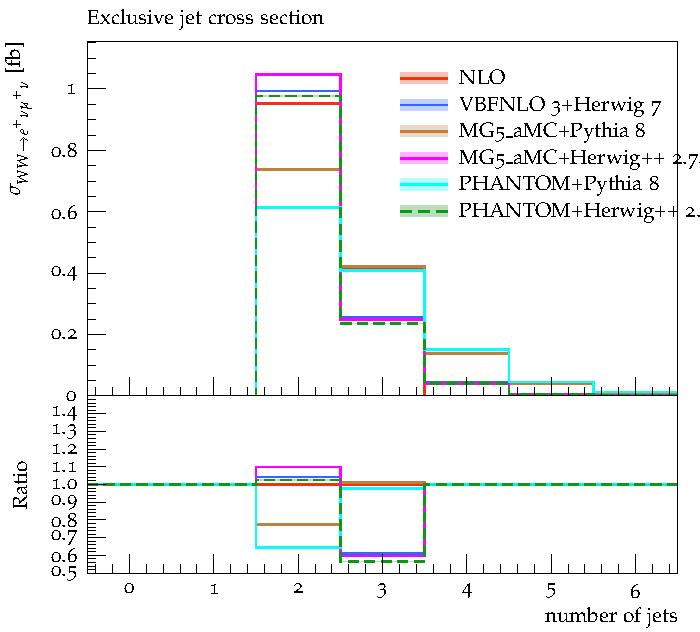
\includegraphics[width=0.47\textwidth]{figures/LOPS/jetsexclusive.pdf}
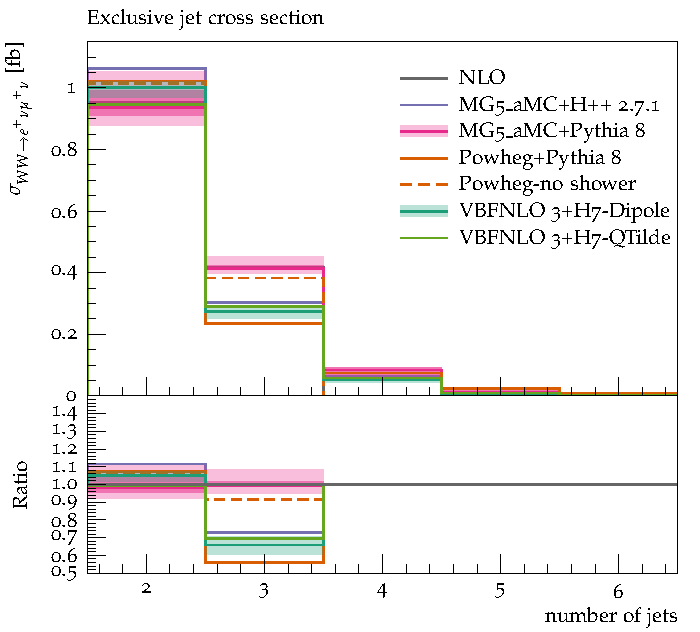
\includegraphics[width=0.47\textwidth]{figures/NLOPS/jetsexclusive.pdf}
\caption{Exclusive jet multiplicity from predictions matched to parton shower, at LO (left) or NLO (right) accuracy, compared with the fixed-NLO result computed with {\sc VBFNLO}. At NLO+PS accuracy, for
    {\sc VBFNLO}+{\sc Herwig7-Dipole}, the three-point scale uncertainties are shown, while for {\sc MG5\_aMC}+{\sc Pythia8} the darker and lighter bands correspond  
    respectively to the nine-point scale uncertainty and the scale and PDF uncertainties combined linearly. }
\label{fig:PSnjet}
\end{figure*}
 
\begin{figure*}[hbt]
\centering
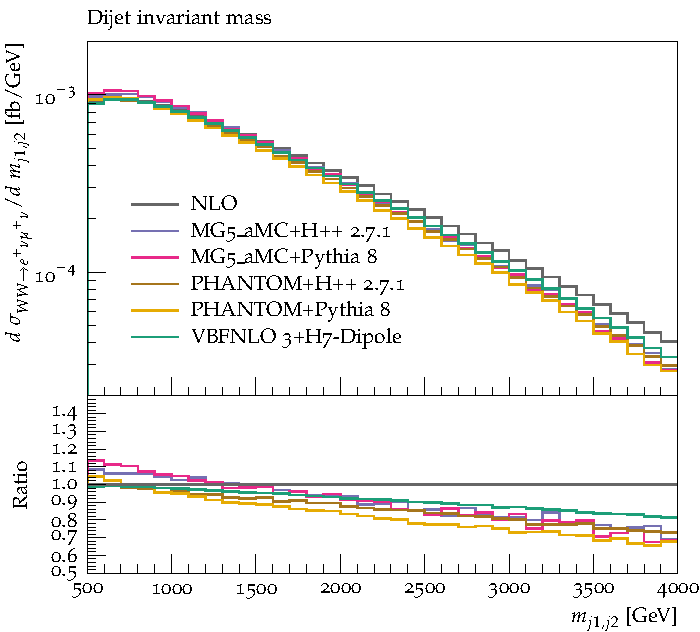
\includegraphics[width=0.47\textwidth]{figures/LOPS/m_jj.pdf}
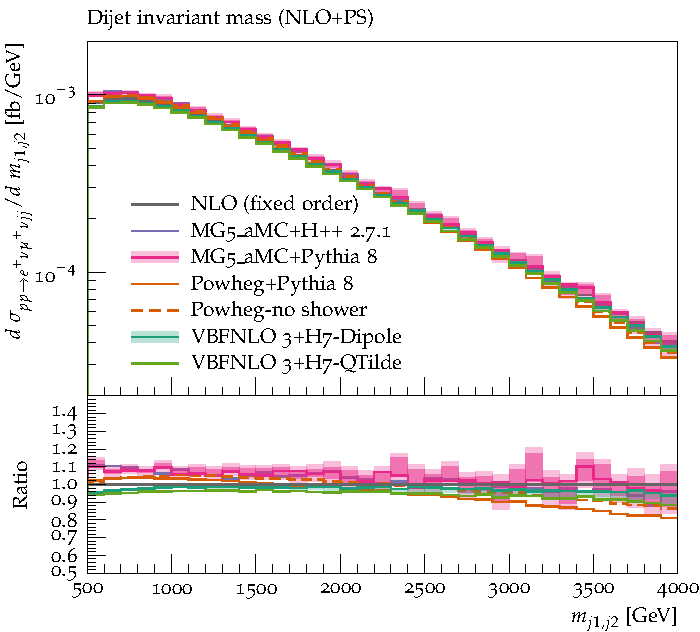
\includegraphics[width=0.47\textwidth]{figures/NLOPS/m_jj.pdf}
\caption{Same as in Fig.~\protect\ref{fig:PSnjet}, for the invariant mass of the two tagging jets.}
\label{fig:PSmjj}
\end{figure*}

The next observable that we study is the invariant mass of the two tagging jets, shown in Fig.~\ref{fig:PSmjj}. For this observable, both at LO+PS and NLO+PS,
the spread of predictions matched with parton shower is rather small
($\lesssim 10\%$, if one compensates for the 6\% width effect for {\sc MG5\_aMC}); LO+PS predictions tend to be significantly softer than the fixed NLO one, with an effect of
about -30\% at the end of the displayed range. At NLO+PS, this effect is much more mitigated, owing to the better description of the first QCD emission which is now driven by the real-emission matrix element.
 
The rapidity difference between the two tagging jets, shown in Fig.~\ref{fig:PSdyjj}, has some similarities to the invariant-mass distribution: at LO+PS all predictions,
except for {\sc VBFNLO3+Herwig7} where the effect is mitigated, show the tendency to deplete the large-separation region with respect to the fixed-order prediction, in a
quantitatively similar way. At NLO+PS, when the extra radiation is described by the real matrix element, such an effect is greatly reduced. A notable
exception is the {\sc Powheg-Box} prediction, which still shows a suppression at large separations: since such a suppression is already there for the {\sc Powheg-no shower} sample,
it is very likely that it is driven by the way the first emission is generated. A minor effect in the same direction is visible in the last two bins of the
{\sc MG5\_aMC+Herwig++} prediction (although with rather large statistical uncertainties).



The transverse momentum of the hardest and second-hardest jets are shown in Figs.~\ref{fig:PSpt1} and~\ref{fig:PSpt2}, respectively. In general, for both observables,
predictions from different tools agree rather well with each other, with a spread at most at the 10\% level. At LO+PS, typically the transverse-momentum spectra are softer than
the fixed-NLO ones, and this effect is more marked for the second-hardest jet which, as expected, is more sensitive to the description of the extra radiation. Again, this
effect is mitigated by NLO corrections. The only feature that may be worth noticing among the NLO+PS predictions is the tendency of the {\sc Powheg-Box} to suppress the
hardest-jet spectrum at low transverse momentum ($\ptsub{\Pj_1}<100 \GeV$).\\
If we consider the rapidity of the second jet, Fig.~\ref{fig:PSy2}, we observe again rather small differences among tools, with the tendency towards a general
stabilisation at NLO+PS. However, some (small) differences in the shape remain at NLO+PS, which are worth to be briefly discussed: predictions
obtained with {\sc MG5\_aMC} are very close to the fixed-order prediction; the {\sc Powheg-Box}\ displays an enhancement of the central region, and a consequent suppression in the
peripheral region, while {\sc VBFNLO} shows an opposite behaviour. However, the effect is rather small, with the largest departure from the fixed-order prediction being
at most $10\%$.\footnote{If the setting {\tt SpaceShower:dipole\-Recoil = on} (discussed in the following of the article) 
is used when {\sc Pythia8}\ is employed together with the {\sc Powheg-Box}, the enhancement at central rapidities and the depletion 
at small value of transverse momentum are partially compensated.}




Finally, focusing on the third jet, we conclude the list of differential observables with showing the Zeppenfeld variable defined in Eq.~\eqref{eq:Zeppenfeld}, Fig.~\ref{fig:PSz3}. This 
variable is closed related to the third jet rapidity, and small (large) value of $z$ correpsond to central (peripheral) rapidities. In general, for observables which involve the third jet, one
can clearly see a degradation of the agreement among the various tools, because of the poorer perturbative description of these observables. The Zeppenfeld variable is 
a striking example: both at LO and NLO, the tendency of {\sc Pythia8} to generate more hard and central radiation, corresponding to low values of $z$,
is clearly visible. Such an effect, which is related to the way {\sc Pythia8} deals with the recoil of the radiation in VBF(VBS)-type processes,
can be mitigated by setting {\tt SpaceShower:dipole\-Recoil = on} in the {\sc Pythia8} input file;\footnote{this requires version $\ge8.230$. 
Note that such a setting is not compatible with the NLO matching
in {\sc MG5\_aMC} (but it is compatible with the {\sc Powheg} matching). Also, this setting has other 
effects, though smaller, on the rapidity spectra of the two hardest jets.} it is interesting to notice that
the effect survives beyond the first emission, as it can be observed by comparing {\sc Powheg-no shower} with {\sc Powheg+ Pythia8}. A similar
behaviour of {\sc Pythia8}
has also been observed in the study of EW production of a $\PZ$ boson in association with two jets (see the recent CMS measurement, 
Ref.~\cite{Sirunyan:2017jej} Figure 12), where the experimental data seem to prefer the description by {\sc Herwig++}. 
The central enhancement
is a bit mitigated if NLO+PS tools are used (compare LO+PS and NLO+PS from {\sc MG5\_aMC+Pythia8} with the fixed-NLO prediction), however even at NLO+PS the central region
($z_{j_3}<0.5$) is cursed by huge differences between tools. Large differences, reaching a factor 2, persist also away from the central region. \\

In conclusion, the comparison of tools including matching with parton-shower clearly shows the benefits of the inclusion of NLO corrections: for most observables described
effectively at NLO accuracy differences between tools are at (or below) the $10\%$ level. 
Some exceptions exist, \emph{e.g.}\ the rapidity separation of the two tagging jets, which
on the one hand clearly suggest not to rely on a single tool/parton shower, and on the other make it worth to investigate more in details the way QCD radiation is
generated, e.g. when fully-differential computations at NNLO will become available (for VBF Higgs production, see Refs.~\cite{Cacciari:2015jma, Cruz-Martinez:2018rod}). It is a remarkable fact that, even for those observables that display small discrepancies,
the theoretical uncertainty obtained via scale variations systematically underestimates the spread of predictions. Again, this stresses the need
 to employ at least two different tools in order to have a conservative estimate of theoretical uncertainties. Finally, the size of discrepancies for observables that are described at a lower perturbative accuracy, notably those related to the third jet, suggest that
experimental analyses should rely as little as possible on those observables and, in any case, use conservative estimate of the theory 
uncertainties. On the one hand, in order to improve the
description of these observables, a simulation of VBS+j at NLO accuracy, currently unavailable but within the reach of modern 
automated tools, is certainly desirable; on the other hand, measurements of processes with similar 
color flow (EW production of a single vector boson plus jets,
VBF, \ldots) can certainly help in order to discriminate which tools perform better in the comparison with data~\cite{Aaboud:2017emo,Sirunyan:2017jej}.

\begin{figure*}[hbt]
\centering
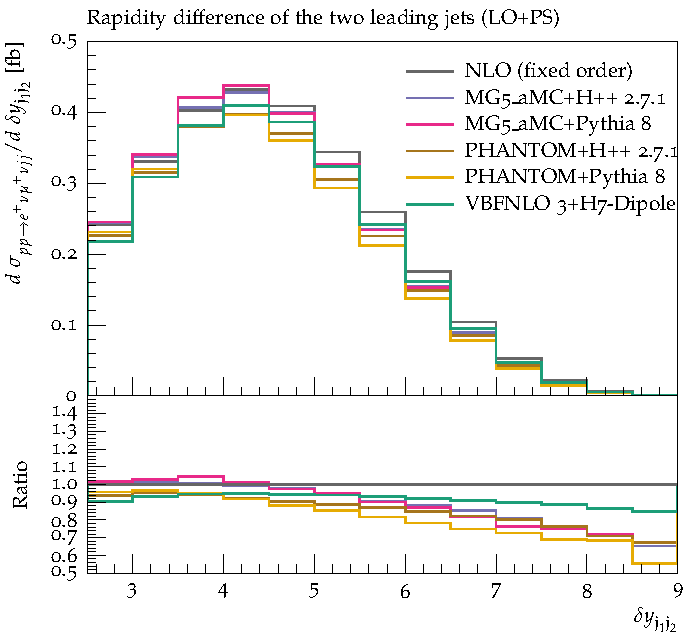
\includegraphics[width=0.47\textwidth]{figures/LOPS/Deltay_jj.pdf}
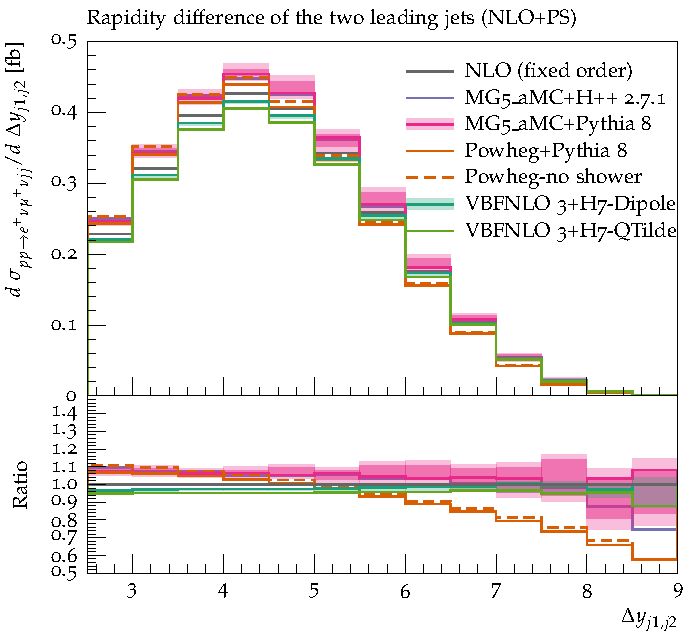
\includegraphics[width=0.47\textwidth]{figures/NLOPS/Deltay_jj.pdf}
\caption{Same as in Fig.~\protect\ref{fig:PSnjet}, for the rapidity separation of the two tagging jets.}
\label{fig:PSdyjj}
\end{figure*}

\begin{figure*}[hbt]
\centering
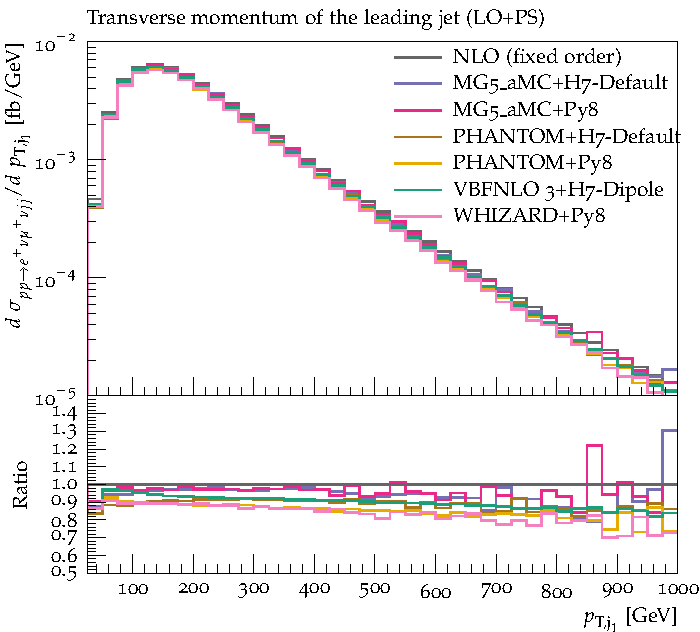
\includegraphics[width=0.47\textwidth]{figures/LOPS/pT_j1.pdf}
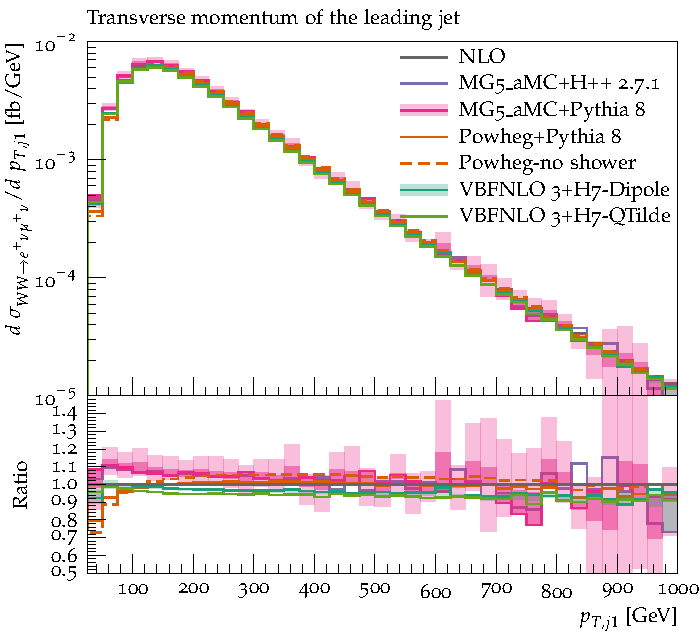
\includegraphics[width=0.47\textwidth]{figures/NLOPS/pT_j1.pdf}
\caption{Same as in Fig.~\protect\ref{fig:PSnjet}, for the transverse momentum of the hardest jet.}
\label{fig:PSpt1}
\end{figure*}

\begin{figure*}[hbt]
\centering
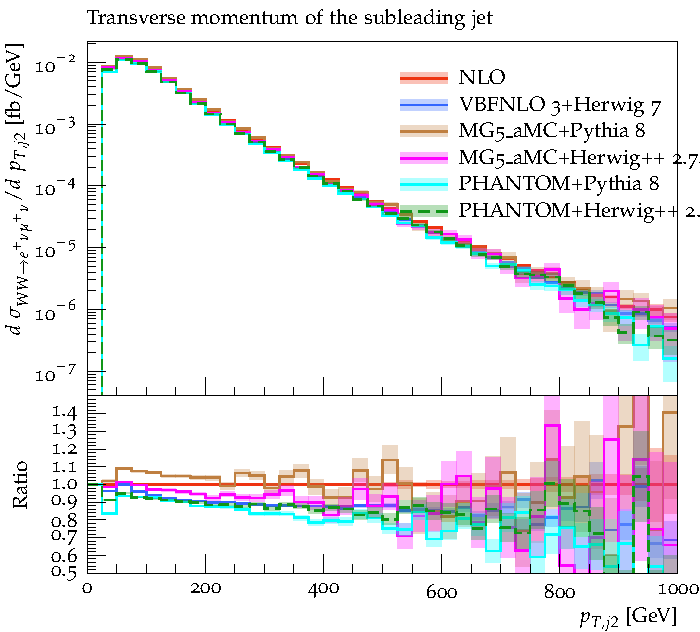
\includegraphics[width=0.47\textwidth]{figures/LOPS/pT_j2.pdf}
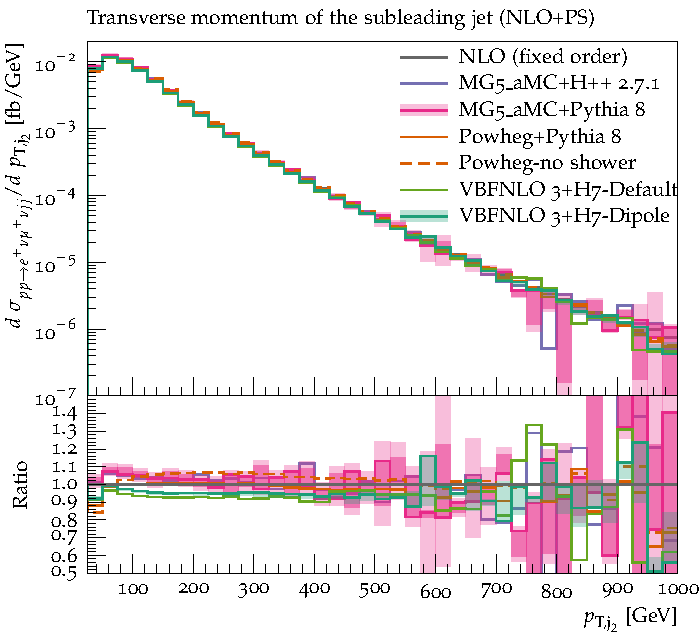
\includegraphics[width=0.47\textwidth]{figures/NLOPS/pT_j2.pdf}
\caption{Same as in Fig.~\protect\ref{fig:PSnjet}, for the transverse momentum of the second-hardest jet.}
\label{fig:PSpt2}
\end{figure*}

\begin{figure*}[hbt]
\centering
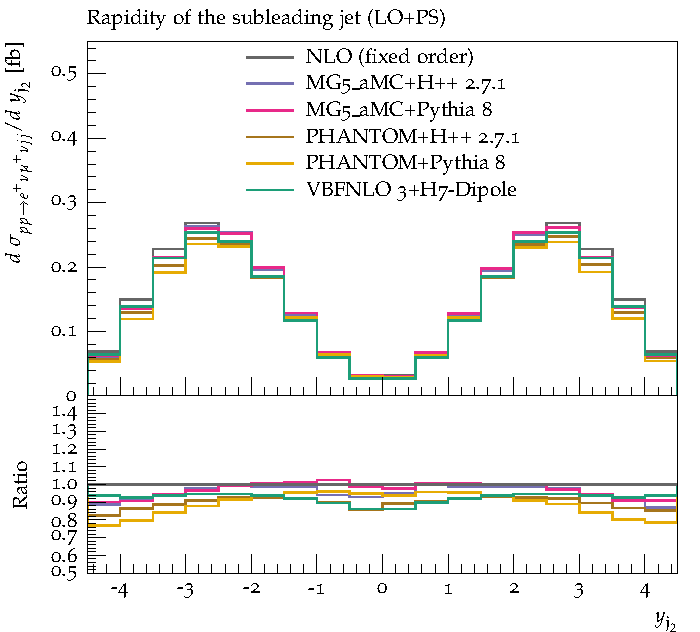
\includegraphics[width=0.47\textwidth]{figures/LOPS/y_j2.pdf}
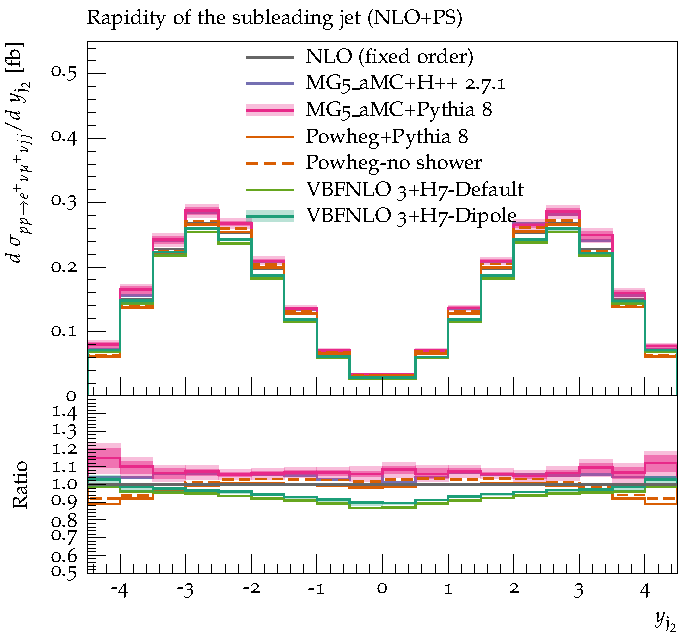
\includegraphics[width=0.47\textwidth]{figures/NLOPS/y_j2.pdf}
\caption{Same as in Fig.~\protect\ref{fig:PSnjet}, for the rapidity of the second-hardest jet.}
\label{fig:PSy2}
\end{figure*}

\begin{figure*}[hbt]
\centering
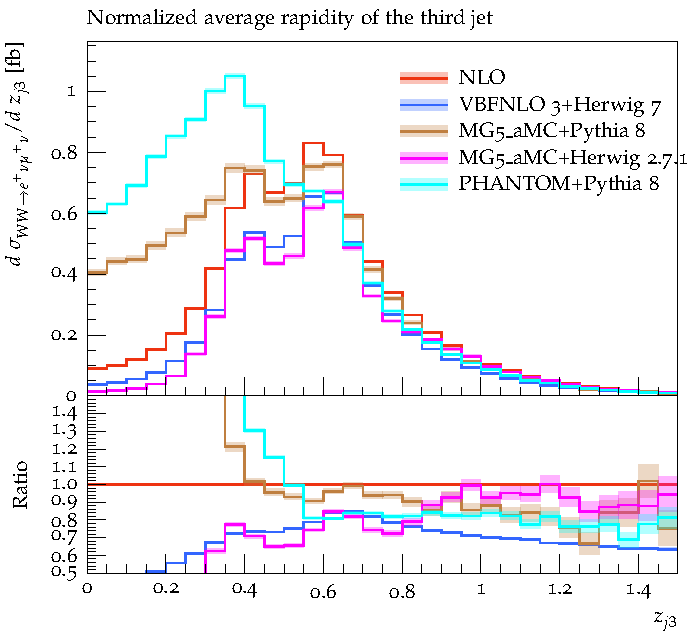
\includegraphics[width=0.47\textwidth]{figures/LOPS/z_j3.pdf}
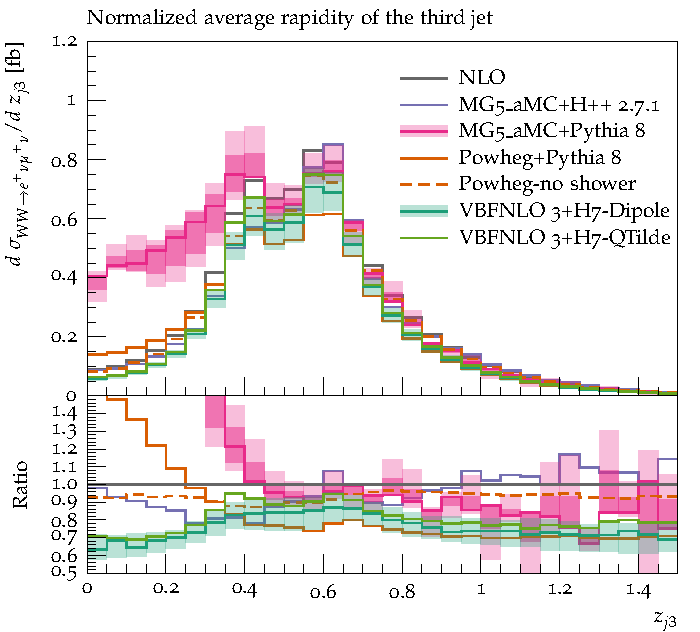
\includegraphics[width=0.47\textwidth]{figures/NLOPS/z_j3.pdf}
\caption{Same as in Fig.~\protect\ref{fig:PSnjet}, for the $z$ variable of the third-hardest jet.}
\label{fig:PSz3}
\end{figure*}


\section{Conclusion}
\label{sec:conclusion}

In the present article, a detailed study of the process $\Pp\Pp\to\mu^+\nu_\mu{\rm e}^+\nu_{\rm e}\,\Pj\Pj+\mathrm{X}$ at the LHC has been presented, 
mainly focused on the electroweak production mechanism which involves the scattering of massive vector-bosons.
Until very recently, when the complete calculation became available for the NLO QCD corrections (order $\mathcal O (\alphas\alpha^6)$),
the so-called VBS approximation was the standard for this kind of simulations. For this reason, various theoretical predictions 
have been compared to the full computation, both in a typical VBS fiducial region and also in more inclusive phase-space.
We have precisely quantified the differences that arise for several physical observables, 
in particular for the di-jet invariant mass and the rapidity-separation of the leading two jets.
This is the first time that such an in-depth study is performed.
%%%%and should be representative of the quality of the approximations for other VBS signatures.
Besides the study of fixed-order predictions, we have also investigated the impact of parton shower.
To that end, several LO and NLO event generators 
which are able to perform matching to parton showers have been employed, and various observables have been thoroughly compared.
While in general observables which are described at NLO accuracy show reasonable agreement among the tools, larger differences can 
appear for those observables described at a lower accuracy, such as those that involve the third jet.
These differences appear in the central region where for VBS, and are the largest for those simulations which employ {\sc Pythia8}.
\MP{This sentence does not make sense (one part probably missing)}.
The effect
has been understood, and it can be partially mitigated by changing the recoil scheme of the parton shower. These findings make it worth 
to further investigate these issues not only in the theoretical community, but also by experimental collaborations, for example by 
measuring related observables for similar processes.

%The results presented here are exclusively theoretical.
%Nonetheless, they should raise significant interests in the experimental collaborations.
The last part of our work is devoted to 
 remarks and recommendations concerning the usage of theoretical predictions by experimental collaborators.
\begin{itemize}
    \item As found in Ref.~\cite{Biedermann:2017bss}, the NLO EW corrections of order $\mathcal{O}{\left(\alpha^{7}\right)}$ are 
        the dominant NLO contribution to the process $\Pp\Pp\to\mu^+\nu_\mu{\rm e}^+\nu_{\rm e}\,\Pj\Pj+\mathrm{X}$.
        It is thus highly desirable to combine them with NLO-QCD predictions matched with parton shower, or at least that they are accounted for
        by experimental analyses. Since, as shown in Ref.~\cite{Biedermann:2016yds}, 
        these large EW corrections originate from the Sudakov logarithms which factorise, we recommend to combine them with QCD 
        corrections in a multiplicative way. The estimate of missing higher-order EW corrections can be done, 
        in a first approximation, by considering $\pm \delta^2_{\rm NLO EW}$,\footnote{The quantity $\delta_{\rm NLO EW}$ through the relation $\sigma_{\rm NLO EW} = \sigma_{\rm LO} \left(1+ \delta_{\rm NLO EW}\right).$} while the missing higher-order mixed QCD-EW corrections 
        can be estimated by taking the difference between the multiplicative and additive prescriptions.
        For more detailed studies of the combination of QCD and EW higher-order corrections, see
        \emph{e.g.}\, Ref.~\cite{Czakon:2017wor} in the context of top-pair production, or Ref.~\cite{Lindert:2017olm} for SM 
        backgrounds for dark matter searches at the LHC.
    \item For the typical fiducial region used by experimental collaborations for their measurements, 
        the agreement between the approximations and the full calculation is certainly satisfactory given 
        the current experimental precision, as well as the one foreseen for the near future \ZM{references, etc}.
        Nonetheless, care has to be taken when using such approximations, in particular if more inclusive phase-space cuts are used.

%{\bf MZ there are many repetitions here} \BJ{I would suggest to remove the following paragraph as it repeats what was already said before.}
%Concerning predictions that include parton shower, we have shown that for observables defined at NLO, the differences are reasonable.
%On the other hand, for observables only defined at NLO-QCD, such as the ones related to the third hardest jet, large differences can arise between different parton-shower algorithms.
%Therefore, jet-veto procedures or selections based on extra radiation should be avoided as they carry rather large uncertainties.

    \item In addition to the standard interpretation of EW signal versus QCD background, 
        combined measurements should also be presented as they are better defined theoretically. In fact, while at LO 
        the interference term can be included in the background component, at NLO the separation of EW and QCD components become more blurred, as, \emph{e.g.}\,
        at the order $\mathcal{O}{\left(\alphas\alpha^{6}\right)}$ both types of amplitudes contribute.
        Therefore, a combined measurement including the EW, QCD, and interference contributions is desirable.
        Note that with such a measurement a comparison to the SM would
        be straigtforward and still be sensitive to the EW component.
        In addition the QCD component could be subtracted based on a
        well-defined Monte-Carlo prediction.

    \item Since the inclusion of NLO QCD corrections gives a better control of extra QCD radiations and reduces the ambiguities related to the 
        matching details and/or the parton shower employed, we encourage the use of NLO-accurate event generators in experimental analyses.

    \item The present study has focused on the orders $\mathcal{O}{\left(\alpha^{6}\right)}$ at 
    LO and $\mathcal{O}{\left(\alphas\alpha^{6}\right)}$ at NLO. NLO computations and publicly-available tools also exist for the QCD-induced process~\cite{Rauch:2016pai,Melia:2010bm,Melia:2011gk,Campanario:2013gea,Baglio:2014uba,Biedermann:2017bss,Alwall:2014hca}.

    \item For practical reasons, we have focused on the ${\rm W}^+{\rm W}^+$ signature. Nonetheless, 
    the observed features 
    (\emph{e.g.}\ validity of the VBS approximation or comparison of theoretical predictions matched to parton shower) should 
    be qualitatively similar for other VBS signatures with massive gauge bosons. For these other signatures, similar quantitative studies should be performed.
\end{itemize}



\section*{Acknowledgements}

The authors are grateful to the members of the VBSCan collaboration for several discussions and comments to this work. The author also thank
the {\sc Pythia8} developers, in particular Stefan Prestel, Torbjorn Sjostrand and Peter Skands for 
discussions and clarifications about the third-jet rapidity spectrum. RF, HSS and MZ thank the {\sc MadGraph5\_aMC@NLO} authors for discussions, and
they are particularly grateful to Valentin Hirschi for comments to this manuscript.

The authors would like to acknowledge the contribution of the COST Action CA16108 which initiated this work.
Moreover, this work was supported by several STSM Grants from the COST Action CA16108.
Many authors acknowledge hospitality from Nikhef, where part of this work has been performed.

BB, AD, and MP acknowledge financial support by the
German Federal Ministry for Education and Research (BMBF) under
contract no.~05H15WWCA1 and the German Science Foundation (DFG) under
reference number DE 623/6-1.
SD and CS acknowledge support by the state of Baden-W\"urttemberg through bwHPC and the German Research Foundation (DFG) through grant no INST 39/963-1 FUGG and grant DI 784/3.
AK acknowledges financial support by the Swiss National Science Foundation (SNF) under contract 200020-175595.
MR acknowledges funding from the European Union's Horizon 2020 research and innovation programme as part of the Marie Sklodowska-Curie Innovative Training Network MCnetITN3 (grant agreement no. 722104).
HSS is supported by the ILP Labex (ANR-11-IDEX-0004-02, ANR-10-LABX-63).
GZ is supported by ERC Consolidator Grant HICCUP (No. 614577).
MZ is supported by the Netherlands National Organisation for Scientific Research (NWO). The work of BJ was supported in part by the Institutional Strategy of the University of T\"ubingen (DFG, ZUK 63) and in part by
the BMBF under contract number 05H2015.


\appendix

\section{Appendix one}


\bibliographystyle{utphys}
\bibliography{article}

\end{document}
